\documentclass[aos,preprint]{imsart}

%% Packages
\RequirePackage{amsthm,amsmath,amsfonts,amssymb,multirow,bbm,autobreak}
%\RequirePackage[numbers]{natbib}
\RequirePackage[authoryear]{natbib} %% uncomment this for author-year bibliography
\RequirePackage[colorlinks,citecolor=blue,urlcolor=blue]{hyperref}
\RequirePackage{graphicx,epstopdf}

\startlocaldefs
%%%%%%%%%%%%%%%%%%%%%%%%%%%%%%%%%%%%%%%%%%%%%%
%%                                          %%
%% Uncomment next line to change            %%
%% the type of equation numbering           %%
%%                                          %%
%%%%%%%%%%%%%%%%%%%%%%%%%%%%%%%%%%%%%%%%%%%%%%
%\numberwithin{equation}{section}
%%%%%%%%%%%%%%%%%%%%%%%%%%%%%%%%%%%%%%%%%%%%%%
%%                                          %%
%% For Axiom, Claim, Corollary, Hypothezis, %%
%% Lemma, Theorem, Proposition              %%
%% use \theoremstyle{plain}                 %%
%%                                          %%
\newtheorem{axiom}{Axiom}
\newtheorem{claim}[axiom]{Claim}
\newtheorem{theorem}{Theorem}[section]
\newtheorem{lemma}[theorem]{Lemma}
\newtheorem{assumption}[theorem]{Assumption}
%%%%%%%%%%%%%%%%%%%%%%%%%%%%%%%%%%%%%%%%%%%%%%
%\theoremstyle{plain}
%\theoremstyle{remark}
\theoremstyle{remark}
\newtheorem{definition}[theorem]{Definition}
\newtheorem*{remark}{Remark}
\newtheorem{example}{Example}
\newtheorem*{fact}{Fact}
%%%%%%%%%%%%%%%%%%%%%%%%%%%%%%%%%%%%%%%%%%%%%%
%%                                          %%
%% For Assumption, Definition, Example,     %%
%% Notation, Property, Remark, Fact         %%
%% use \theoremstyle{remark}                %%
%%                                          %%
%%%%%%%%%%%%%%%%%%%%%%%%%%%%%%%%%%%%%%%%%%%%%%
%%%%%%%%%%%%%%%%%%%%%%%%%%%%%%%%%%%%%%%%%%%%%%
%% Please put your definitions here:        %%
%%%%%%%%%%%%%%%%%%%%%%%%%%%%%%%%%%%%%%%%%%%%%%

\endlocaldefs

\begin{document}

\begin{frontmatter}
\title{Manifold Fitting and Projection via Quadratic Approximation}
%\title{A sample article title with some additional note\thanksref{t1}}
\runtitle{Second Order Form Manifold Fitting and Applications}
%\thankstext{T1}{A sample additional note to the title.}

\begin{aug}
%%%%%%%%%%%%%%%%%%%%%%%%%%%%%%%%%%%%%%%%%%%%%%
%%Only one address is permitted per author. %%
%%Only division, organization and e-mail is %%
%%included in the address.                  %%
%%Additional information can be included in %%
%%the Acknowledgments section if necessary. %%
%%%%%%%%%%%%%%%%%%%%%%%%%%%%%%%%%%%%%%%%%%%%%%
\author[A]{\fnms{First} \snm{Author}\ead[label=e1]{first@somewhere.com}},
\author[B]{\fnms{Second} \snm{Author}\ead[label=e2,mark]{second@somewhere.com}}
\and
\author[B]{\fnms{Third} \snm{Author}\ead[label=e3,mark]{third@somewhere.com}}

%\author[A]{\fnms{Zheng} \snm{Zhai}\ead[label=e1]{first@somewhere.com}}
%and
%\author[B]{\fnms{Zhigang} \snm{Yao}\ead[label=e2,mark]{second@somewhere.com}}
%%\and
%%\author[B]{\fnms{Third} \snm{Author}\ead[label=e3,mark]{third@somewhere.com}}
%%%%%%%%%%%%%%%%%%%%%%%%%%%%%%%%%%%%%%%%%%%%%%
%% Addresses                                %%
%%%%%%%%%%%%%%%%%%%%%%%%%%%%%%%%%%%%%%%%%%%%%%
%\address[A]{Department,University or Company Name,\printead{e1}}

%\address[B]{Department, University or Company Name,\printead{e2,e3}}
\affiliation{National University of Singapore}
\end{aug}
\begin{abstract}
%Modern statistics encounters with the high dimensional data in ambient space in almost everywhere. Although the data point usually represents it- self as a long vector or a big matrix, in principle they all can be viewed as points on or near an intrinsic manifold. How to estimate the underlying manifold has been emerging as a great interest to the statistics community. 
In this paper, we propose to fit the manifold by a quadratic function defined on the tangent space with a specific form. Compared with the existing linear approximation methods, the quadratic approximation approach can fit the unknown manifold with higher precisions. Because more complicated function is adopted in our manifold fitting process, the pulling back approach turns from the linear least square problem into a nonlinear quartic minimization problem. By bringing in the auxiliary function, we solve the quartic by repeatedly solving a series of quadric minimization problems. Numerical experiments demonstrate that our method has a very strong recovery capability compared with the current works.
\end{abstract}

\begin{keyword}[class=MSC2020]
\kwd[Primary ]{00X00}
\kwd{00X00}
\kwd[; secondary ]{00X00}
\end{keyword}

\begin{keyword}
\kwd{Manifold fitting}
\kwd{manifold projection}
\kwd{quadratic approximation}
\end{keyword}

\end{frontmatter}
%%%%%%%%%%%%%%%%%%%%%%%%%%%%%%%%%%%%%%%%%%%%%%
%% Please use \tableofcontents for articles %%
%% with 50 pages and more                   %%
%%%%%%%%%%%%%%%%%%%%%%%%%%%%%%%%%%%%%%%%%%%%%%
%\tableofcontents
\section{Introduction}

The data residing in the high-dimensional ambient space often have some low-dimensional structure, because of the principal factors which affect the intrinsic generation process are often very limited. The locations of earthquakes or volcanos which caused by the crustal movement can be thought as the points residing on the one-dimensional manifold or the principal flow \cite{panaretos2014principal,davenport2010joint}.

In deep learning approach \cite{NIPS2014_5ca3e9b1}, using a network with fine-tuning parameters, we can transfer a very low-dimensional data into a very complicated image which some specific meaning. Also, we can use a simple sentence to generate a vivid picture  by a well-trained network. These phenomena indicate that very huge amount of data in our daily life are low-dimensional.

 
To handle the high-dimensional data, there are mainly two approaches. First, reconstruct the data in the low-dimensional space, such that, the reconstructed data in the low-dimensional space also keeps the relation (such as distance, geometry, affine transformation etc) in high dimensional space. This approach containing lots of classical dimension reduction works, such as LLE \cite{roweis2000nonlinear}, LTSA \cite{zhang2004principal}, Isomap \cite{tenenbaum2000global}, Eigenmap \cite{belkin2003laplacian}.
 
 The other approach try to fit a new smooth manifold by reducing the noise existing in the data. After the fitting process, the true signal will be strengthened and the noise factors will be diminished. Kernel density estimation \cite{genovese2014nonparametric,ozertem2011locally} is a very popular tool for the manifold fitting by transforming the manifold fitting problem into the ridge estimation problem. The ridge is defined as the set of points which satisfy some relation on gradient and Hessian of the density function. Overall, all the manifold fitting process can be considered with two steps. First, estimate the tangent space which is often implemented through the eigenvalue-decomposition of the covariance matrix. Second,  estimate an attraction force which is a  direction which points to somewhere near the manifold, this direction often constructed via the weighted shift-mean approach. By using the subspace constraint mean shift algorithm, we can move the outlier onto the manifold to some degree.
 
 The approximation error for the local affine space will yield an approximate error of $\|\tau\|_2^2$, where $\tau$ is the local coordinate. In other words, when we restrict the error subjects to the condition $\|\tau\|_2^2\leq \epsilon$, the maximum radius of the valid region is with the order of $\epsilon^{1/2}$. In this paper, we propose to approximate the manifold via the quadric function, by adopting this strategy, the approximation error will become $\|\tau\|_2^3$.  With the same precision requirement $\epsilon$, we have the maximum radius of our interested region is of the order $\epsilon^{1/3}$. Normally, $\epsilon$ is some scalar less than $1$, in this way, the quadratic approximation is a better approximation compared with the tangent affine plane.That is to say, to achieve the same precision, we will need much less times of fitting process.

A good approximation of the underlying manifold is the first step in our manifold fitting problem. The second important step needs to project the noisy data onto the fitted manifold which we obtained in the first step. Here, the term `project' has two meanings. First, the distance should be minimum, second, the direction of the projection should be perpendicular with the tangent place of the fitted manifold. A major reason for the linear approximation to be very widely used is the form of projection yields a very simple linear least square problem.


%\begin{figure}[h] %  figure placement: here, top, bottom, or page
%   \centering
%   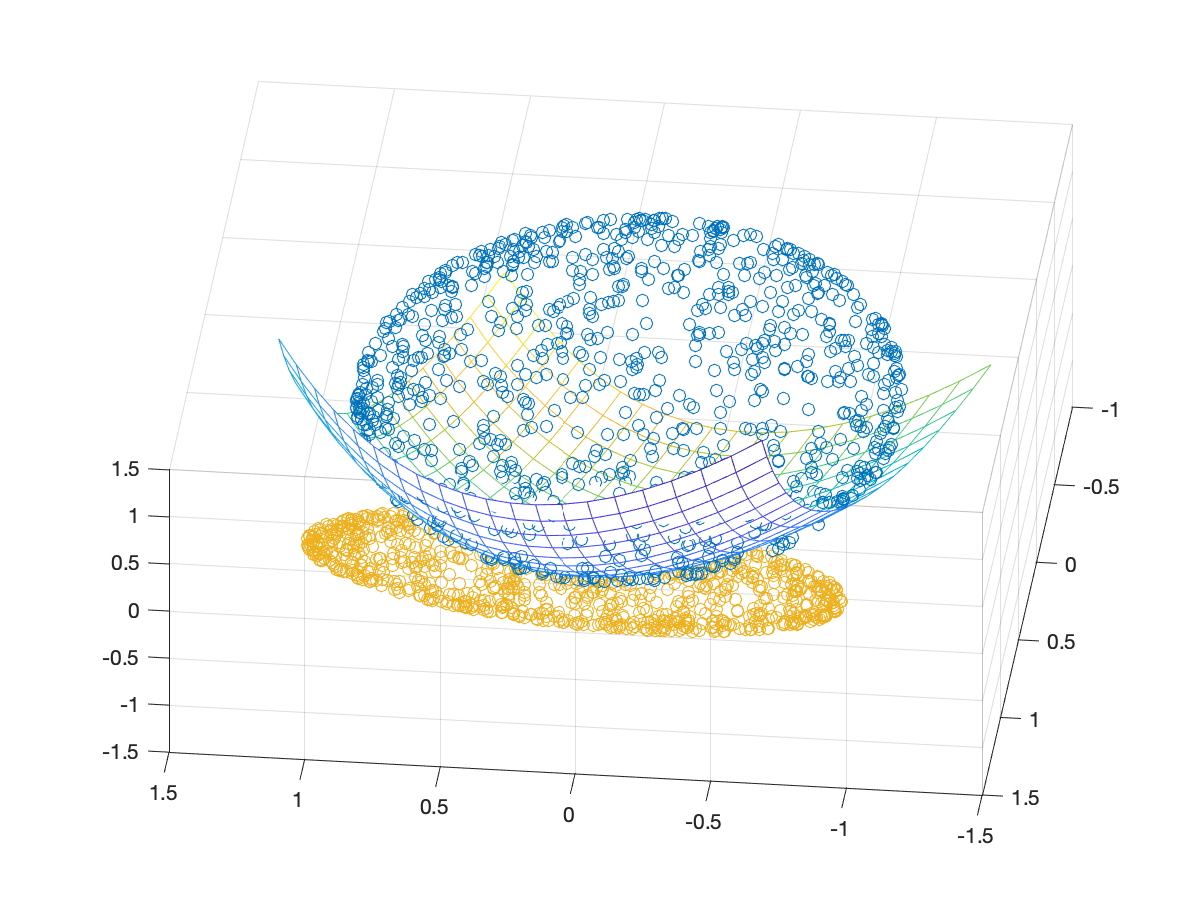
\includegraphics[width=3in]{demo.eps} 
%   \caption{ Fitting a manifold with the elliptical paraboloid surface}
%   \label{3-D paraboloid}
%\end{figure}

\subsection{Fitting Model}
In this paper, we are not concentrating on finding the representation of $\phi(\tau)$ under the noiseless assumption. Instead, we assume to have the observations drawn from some low-dimensional manifold and disturbed by some noise, i.e
\[
x_i = \tilde{x}_i+\epsilon_i, \quad \tilde{x}_i \in \cal M
\] 
where $\epsilon_i$ is some noise which obeys some distribution, such as multi-dimensional gaussian noise.

Since the observations $\{x_i, i=1:n\}$ are discrete distributed, the idea of manifold fitting aims at generalizing the discrete data and obtaining a low-dimensional approximation of the dataset. The manifold fitting approach can be written as a parameter estimation problem under the observation and the constrained model $\cal G$.
\begin{equation}\label{estimator1}
 \theta_* =\arg \min_\theta  \sum_i {\rm Loss}(x_i, {\cal G}, \theta ),
\end{equation}
where $\cal G$ represents the abstract model and $\theta$ represents the parameters within the model $\cal G$. Different models (such as linear or nonlinear) correspond to different $\cal G$. When we obtain our best parameter $\theta_*$ from \eqref{estimator1}, we can use the model ${\cal G}(\theta_*)$ to refine the outlier $x$ using $P_{{\cal G}(\theta_*) }(x)$ via solving the following minimization problem:
\[
P_{{\cal G}(\theta_*) }(x) = \arg \min_{y\in {\cal G}(\theta_*) } \|x-y\|_2.
\]
 
The works such as \cite{genovese2014nonparametric,ozertem2011locally} all focus on how to get a better affine space to locally approximate the distribution of the data, i.e, ${\cal G}(\theta)$ is a linear model. However, at far as we know, the result of linear approximation approach relies heavily on the selection of the origin point (the red dot in Figure \ref{Comparison} ). An origin selected with good quality will surly improve the ability of recovery of the projection.

\subsection{Manifold Parameterization}
For any manifold $\cal M$ and any point $x_0\in \cal M$, there is a corresponding twice differentiable function $\phi_{x_0}(\tau)$ 
\begin{figure}[h!] %  figure placement: here, top, bottom, or page
   \centering
   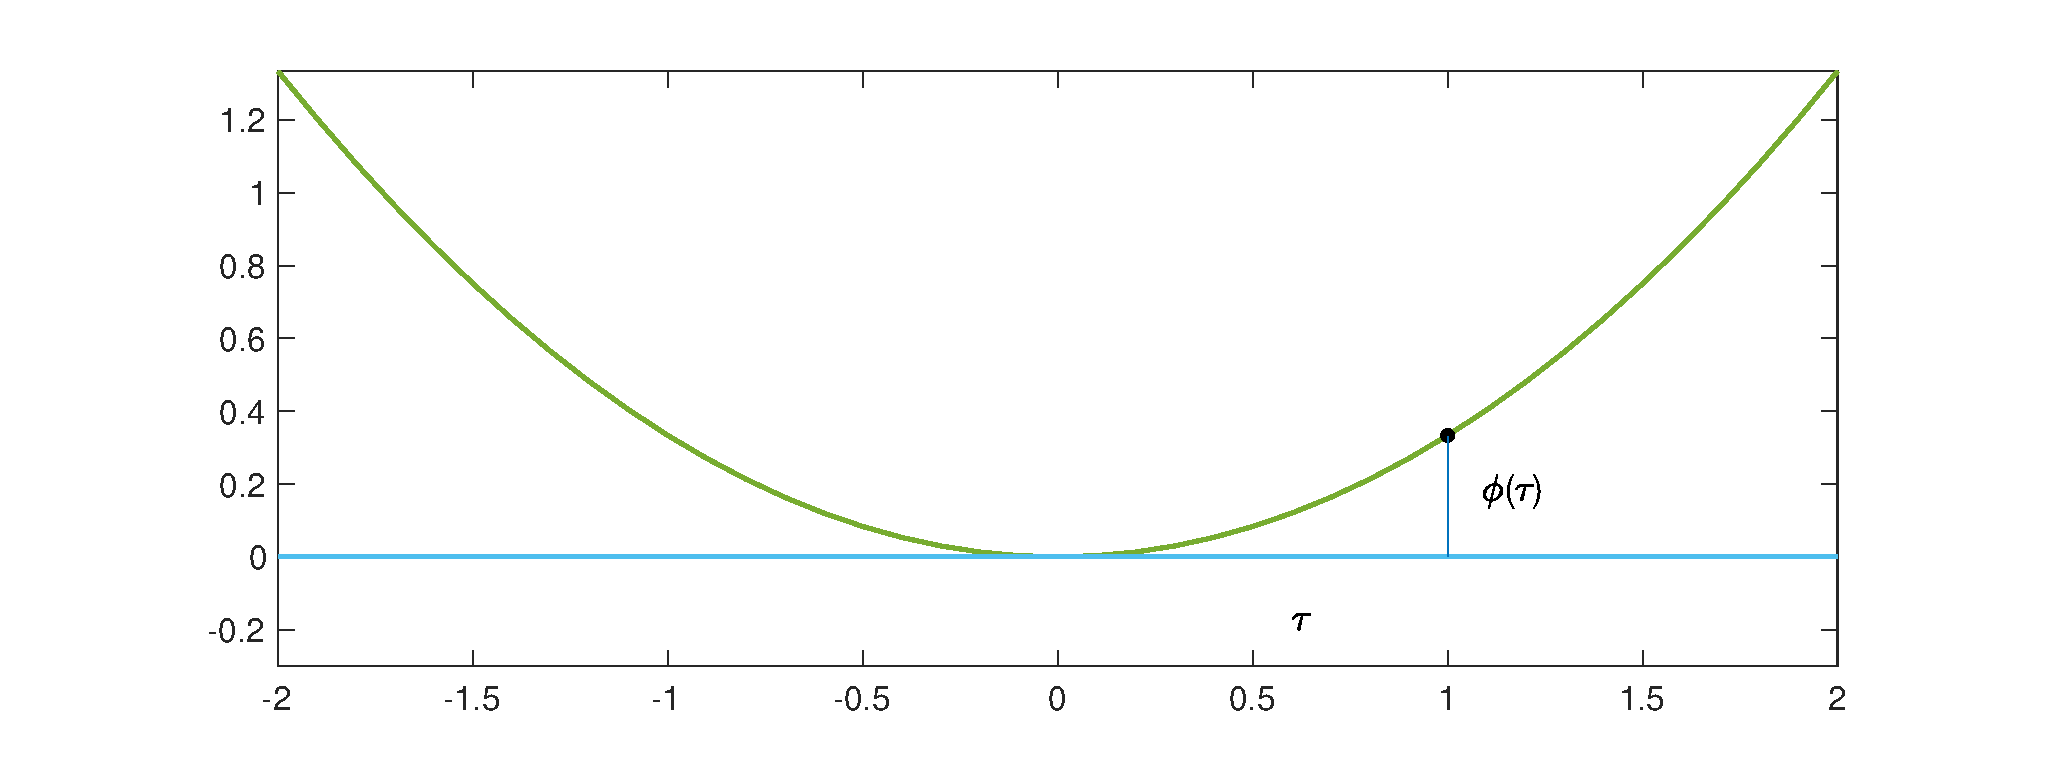
\includegraphics[width=5in]{demo_phi.eps} 
   \caption{Geometric interpretation of $\tau$ and $\phi(\tau)$ for a  1-D manifold embedded in 2-D}
   \label{3-D paraboloid}
\end{figure}
\[
\phi_{x_0}(\tau):{\mathbb R}^d\rightarrow {\mathbb R}^{D-d},
\]
such that every point within a local domain ${\cal D}_{x_0}(r)$ of $\cal M$, can be written with a parameterization form of 
\begin{equation}\label{manifold}
x(\tau)=  x_0 + U_{x_0} \tau+ U_{x_0}^{\perp} \phi_{x_0} (\tau),
\end{equation}
where the columns of $U_{x_0}$ are the basis on the tangent space and the columns in $U_{x_0}^{\perp}$ are the basis on the normal space. 


In other words, corresponding to $x_0$ and $\cal M$, there is some radius $r$, such that:
\begin{equation}\label{model}
 {\cal M}\cap {\cal D}_{x_0}(r) =  \{y | y =  x_0 + U_{x_0} \tau+ U_{x_0}^{\perp} \phi_{x_0} (\tau), \tau\in {\mathbb R}^d\}\cap {\cal D}_{x_0}(r).
\end{equation}
where ${\cal D}_{x_0}(r) = \{x|\|x-x_0\|\leq r\}$, $\phi_{x_0}(\tau)=[\phi_{x_0}^{d+1}(\tau),...,\phi_{x_0}^{D}(\tau)]^T$  is the function defined on the tangent space, the range of $\phi_{x_0}(\tau)$ represents the coordinate in the normal space and $\tau$ is the local coordinate in the tangent space.

\begin{figure}[t!] %  figure placement: here, top, bottom, or page
   \centering
   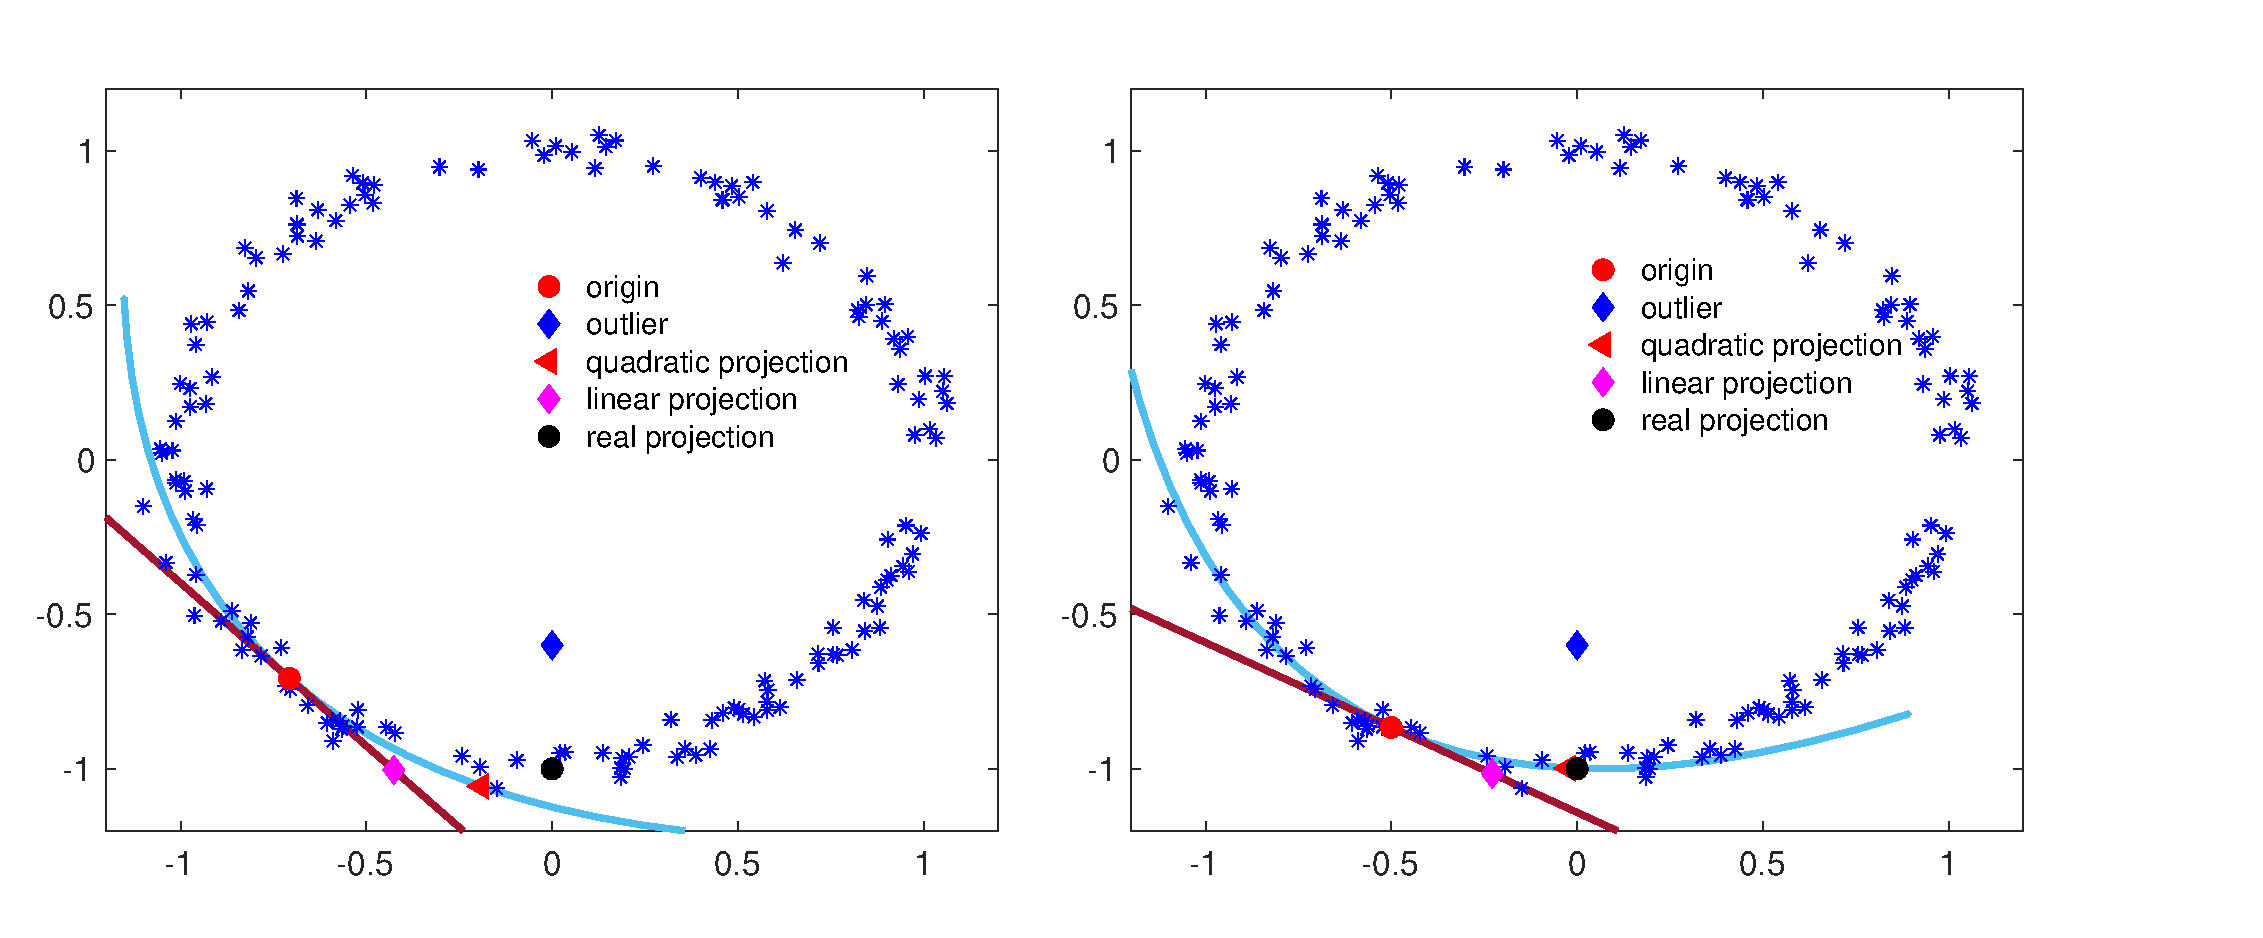
\includegraphics[width=\linewidth]{democ3.eps} 
   \caption{The reliance of the origin point in the process of manifold fitting and projection}
   \label{Comparison}
\end{figure}
To demonstrate the difference behaviors corresponding to the linear and quadratic fitting approaches, we give a toy fitting case in Figure \ref{Comparison} with different origins. The origin $x_0$ (the red dot) in the left figure is farther away from the true projection (the black dot) than that in the right figure.  This example shows the effect of the different fitting errors, which is $O(\|\tau\|_2^2)$ and $O(\|\tau\|_2^3)$ corresponding to the linear and quadratic forms, respectively. From this case, we know that since the linear approximation approach yields a lower-order error, the linear approach relies on a good origin heavily than the quadratic form.
 

In this paper, we transfer our manifold fitting problem into finding an approximation version of $\phi_{x_0}(\tau)$ through a deep analysis on the characteristic of it. We also show the dominant term for Taylor expansion of $\phi_{x_0}(\tau)$ can be written as a quadratic form of a tensor acting on $\tau$, i.e, $\nabla\nabla \phi_{x_0}(\tau)|_{\tau=0}(\tau,\tau)$, where $\nabla\nabla\phi_{x_0}(\tau)|_{\tau=0}$ is a third-order tensor with shape of $d\times d\times (D-d)$.  

In addition, we show that, by adopting the dominant term in the Taylor expansion of $\phi_{x_0}(\tau)$,  the nonlinear function $\phi_{x_0}(\tau)$ can be locally simplified as a quadratic form of ${\cal A}(\tau,\tau)$, where $\cal A$ is the empirical estimation of $\nabla\nabla \phi_{x_0}(\tau)|_{\tau=0}$. The unknown parameters $\cal A$ can be obtained via a linear least square problem. After obtaining the representation of $x_{\cal A}(\tau)$, we also develop a projection strategy to refine the outlier point $\bar{x}$ by projecting it onto our fitted manifold $\cal M_A$. Furthermore, we show the projection of $\bar{x}$ onto $\cal M_A$ can be achieved by repeatedly solving a series of linear least square problems.
\section{Related work}
\subsection{Manifold approximation by Linear Methods}
Fitting the manifold with linear methods corresponds to setting $\phi_{x_0}(\tau)$ in \eqref{manifold} equals to zero. Then, the problem becomes to find $x_0$ and $U_{x_0}$ such that we can approximate the manifold linear around $x_0$ by a linear parameterization form
\[
x(\tau) = x_0 + U_{x_0} \tau
\]
Note that, the function $x(\tau)$ is a local approximation of $\cal M$ at $x_0$. The choice of $x_0$ depending on our interest area, such that, if we want to project an outlier $\bar{x}$ onto the manifold, $x_0$ can be selected as the nearest point $x_0$ on $\cal M$, such that 
\[
\|x_0-\bar{x}\|_2=\min_{x_0\in \cal M} \|x_0-\bar{x}\|_2
\]

There are lots of works which approximate the basis $U_{x_0}$ in the tangent space by a linear space approach. 
One approach is to directly fit the manifold by finding the eigenspace of some matrices, e.g the covariance matrix or Hessian of KDE. Then using the eigenvalue-decomposition to get the eigenspace corresponding to the $d$ largest eigenvalues. The Hessian of the the classical KDE approach shares the same eigenspace of 
\[
C(\bar{x}) = \sum_i K_h(\bar{x},x_i) (x_i-\bar{x})(x_i-\bar{x})^T
\]
If transformed by the concave increasing function $\log$ with respect to the KDE function, the deterministic term in the Hessian matrix will become 
\[
C(\bar{x}) = \sum_i K_h(\bar{x},x_i) (x_i-c(\bar{x}))(x_i-c(\bar{x}))^T
\]
where $c(\bar{x})$ is the weighted shift mean vector. In this case, using the basis (consisting of the columns of $U_d$) corresponding to the largest $d$ eigenvalues of the covariance matrix $C(\bar{x})$. 

When we use the locally shift mean to replace the origin $x_0$,  the affine space yields the form as
\[
x(\tau) = c(\bar{x}) + U_d\tau,
\]
where $\tau$ is the coordinate in the $d$-dimensional space. The projection onto the $x(\tau)$ of $\bar{x}$ is
 \[
\bar{x}+U_{\perp}U_{\perp}^T(c(\bar{x})-\bar{x}) = c(\bar{x})+ U_dU_d^T(\bar{x} -c(\bar{x}))
\]
There are also complex methods such as \cite{fefferman2018fitting,yao2019manifold} by approximating the normal space at $x$ as a weighted combination of the normal space at each neighbor sample $x_i$ as
\[
A = \sum_i \alpha_i \Pi_i^{\perp}
\]
where $\Pi_i^{\perp}$ is the estimated normal space at the observation $x_i$ and $\alpha_i$ is the weight for $x_i$.
Then the normal space can be obtained from eigenvalue decomposition of $A$ and picking up the eigenvectors corresponding to the $D-d$ largest eigenvalues.
%Usually, the normal space (orthogonal complement of the tangent space) is used to act as a constraint, such that, the iteration of the mean-shift algorithm performs within a proper subspace. This subspace constraint tries to keep the component in the normal space and leave out or diminish the component of scale in the tangent space. All the normal space is obtained from the eigenvalue decomposition of a temporary matrix (Hessian or Combination of Normal Space).
%
% For the ridges obtained from both SCRE and {log}-SCRE (SCRE transformed with a $\log$ function), we need to compute the second derivative for the function to obtain the Hessian matrix $H(x)$ or the corresponding covariance matrix $J(x)$. Then, the projection can be produced from the eigenvalue decomposition, and we can pick the eigenspace corresponding to the smallest D-d eigenvalues. For SCRE, the covariance matrix is $J(x) = \sum_i w(x_i,x)(x_i-x)(x_i-x)^T$. For {log}-SCRE, the covariance matrix is $J(x) = \sum_i w(x_i,x)(x_i-c(x))(x_i-c(x))^T$, where $c(x)$ is the one-step shift mean of $x$.
%
% In our {\it l}-SCRE approach, we build the semidefinite local covariance matrix as $C_{r}(x)=\sum_{i\in {\cal I}_r} w_{h,r}(x_i, x)(x_i-c_r(x))(x_i-c_r(x))^T$. The {\it l}-SCRE has two main advantages. First, the covariance matrix $C_{r}(x)$ in the local area of $B_{{x}}(r)$ is more similar to a low-rank matrix than one in a global area. As a result, we can easily recover the low-dimensional space to approximate $B_{{x}}(r)\cap \mathcal M$. Second, because we restrict our consideration to a small domain, the smooth parameter $h$ can be chosen more easily than before.
%
%Instead of computing the Hessian, the manifold-fitting strategy \cite{fefferman2018fitting}  approximates the normal space at ${x}$ with a weighted combination of projection matrix $\Pi_i^{\perp}$ as $A = \sum_i \alpha_i \Pi_i^{\perp}$ of the normal projection $\Pi_i^{\perp}$ at each point $x_i$ in the neighborhood. Then, the D-d principal components from the eigenvalue decomposition of $A$ is regarded as the projection onto the normal space at ${x}$. The benefit of this approach is that the projection $\Pi_i^{\perp}$ at each point $x_i$ is a constant matrix that does not depend on the location of ${x}$. However, because it is required to approximate a large number of tangent spaces, this approach needs  a considerably large amount of computation resources.
\subsection{Manifold approximation by Nonlinear Least-square Approach}
Using the moving least-square (MMLS) projection approach to approximate the manifold is proposed by \cite{sober2019manifold}. In their work, they choose to approximate the manifold with two steps. 
\begin{itemize}
\item[1.] Given the outlier $x$, find the local coordinates by solving a minimization problem
\[
(\hat{q}(x),\hat{\cal H}(x))= \arg\min_{x-q\perp {\cal H}}  
 \sum_{i=1}^n d^2 (x_i, {\cal H}) \theta(\|x_i-q\|),
\]
where $\cal H$ is the $d$-dimensional affine subspace and $q$ is the origin. The squared distance from $x_i$ to $\cal H$ is $d^2 (x_i, {\cal H}) = \|V^T_{\cal H}(x_i -q)\|_2^2$.
The parameter $\hat{q}$ and $\hat{H}$ is achieved by a repeated minimizing procedure. 

\item[2.]  Using the local coordinate $\tau_i = V^T_{\cal H}(x_i-q)$, fit the polynomial by minimizing
\[
\hat{g} = \min_{p\in \Pi_m^d} \sum_{i=1}^n \|p(\tau_i)-f_i\|_2^2 \theta(\|x_i-q\|),
\]
where $\Pi_m^d$ is the polynomial function class up to order $m$ defined in the $d$-dimensional space. Then, the projection is defined as: $P_m(r) = \hat{g}(0)$. 
\end{itemize}
\subsection{Difference}
Our approach differ with the former approaches in three respects. 
\begin{itemize}
\item[1.] We do not require the origin satisfy $r-q\perp H$ in our approach by simplifying the first step. 
%by give a initial $q$ as the origin of our fitting. 
Since our method is not sensitive to the initial point $q$, by using the initial guess of $q$, $H$ can be obtained by PCA very easily.
\item[2.] We restrict the form of our polynomial which will result in a with very concise form and save lots of extra parameters. The manifold fitting by a second-order paraboloid function has a more concrete form by defining a tensor which has the clear meaning by representing the curvature of our manifold. The tensor can be obtained by solve a linear least square problem in each of the normal dimensions.
\item[3.] The projection of outlier $r$ onto the fitted manifold $\cal M_A$ is not restraint to be the origin point of ${\cal M_A}$. It can be any points $\cal M_A$ as long as the minimum criteria is achieved.
\end{itemize}
The strengths of our method can be summarized as:
\begin{itemize}
\item[1.] By fitting a function with the quadratic form, the curvature of the manifold is considered in our algorithm. Because of the existing of the curvature, the fitted manifold ${\cal M}_{\cal A}$ can approximate the true manifold in a relatively larger scope.
\item[2.] Our algorithm does not rely on the accuracy of the estimated origin point too much, which means a relatively rough estimation of the origin is accessible in our algorithm. Instead of the origin, we just need to get a point (nearby $x$) which is also supposed to be next to the true $\cal M$.
\item[3.] The solution of our algorithm has a clear geometric interpretation via the optimized $\hat{\tau}$.  When we got the local coordinate $\hat{\tau}$, we can think of our projected point $x(\hat{\tau})$ ( the projection onto ${\cal M}_{\cal A}$) as a modification of the origin $x_0$, through,
\[
x(\tau) = U_\perp {\cal A}(\tau,\tau) + U\tau + x_0. 
\]
where $U\tau$ is the modification of $x_0$ in the tangent space and ${\cal A}(\tau,\tau)$ is the modification of $x_0$ in the normal space.
\end{itemize}
\section{Preliminary: Tensor Operation} 
In this section, we give some preliminary knowledge with tensor operation and tensor differentiation. Using tensor notations  will bring in lots of convenience in our notations and discussion.
\subsection{Multiplication}
For a three-order tensor $\cal A$ with the shape of $d\times d\times (D-d)$, 
%As the matrix can be seen as a tensor of order 2. 
we can also think of $\cal A$ as an operator acting on the $d$ or $(D-d)$ dimensional vector space, besides regarding $\cal A$ as a particular array of numbers.
For a vector $\tau \in {\mathbb R}^d$, the tensor $\cal A$ acting on $\tau$ will result in a matrix denoted as ${\cal A}(\tau)$ of shape $d\times (D-d)$, of which the $j,k$-th element is
\[
\{{\cal A}(\tau)\}_{jk} = \sum_i \tau_i {\cal A}_{i,j,k},
\]
which is a weighted combination of the slices in the first dimension of the tensor $\cal A$.
Similarly, for two vectors $\tau,\eta\in {\mathbb R}^d$, the tensor $\cal A$ acting on $\tau,\eta$ will result in a vector denoted as ${\cal A}(\tau,\eta)\in {\mathbb R}^{D-d}$, whose $k$-th element is
\[
\{{\cal A}(\tau,\eta)\}_{k} = \sum_{i,j} \tau_i \eta_j {\cal A}_{i,j,k} .
\]
Clearly, we have the vector ${\cal A}(\tau,\eta)$ can be written as a matrix-vector product by: $ {\cal A}(\tau,\eta) = {\cal A}(\tau)^T \eta$ and the summation with index $i,j$ can also be regarded as an inner product of matrix, i.e, $\{{\cal A}(\tau,\eta)\}_{k}=\langle\tau\eta^T ,{\cal A}_{\cdot\cdot k}  \rangle $ .%, where ${\cal A}(\tau)^T \eta$ is the ordinary matrix-vector multiplication.
\subsection{Differentiation}
For the $(D-d)$ dimensional vector ${\cal A}(\tau,\tau)$, we can take the differential operation with respect to $\tau$. The first derivative of ${\cal A}(\tau,\tau)$ with respect to $\tau$ will result in a matrix of size $d\times (D-d)$ and the second derivative of ${\cal A}(\tau,\eta)$ with respect to $\tau$ and $\eta$ will get the tensor $\cal A$,
\begin{gather*}
\nabla_\tau {\cal A}(\tau,\tau) =  2{\cal A}(\tau) \in \mathbb{R}^{d\times (D-d)},\\
\nabla_\eta \nabla_\tau {\cal A}(\tau,\eta) =  {\cal A}\in  \mathbb{R}^{d\times d\times (D-d)},\\
\nabla_\tau \nabla_\tau {\cal A}(\tau,\tau) =  2{\cal A}\in  \mathbb{R}^{d\times d\times (D-d)}.
\end{gather*}
Noticing that ${\cal A}(\tau,\tau,\iota)$ is a scalar, taking the derivative for $\tau$ twice will result in a symmetric matrix (similar with Hessian)
\begin{gather*}
\nabla_\eta \nabla_\tau {\cal A}(\eta,\tau,\iota) =  {\cal A(\iota)} = \sum_k \iota_k {\cal A}_{\cdot\cdot k}\in \mathbb{R}^{d\times d},\\
\nabla_\tau \nabla_\tau {\cal A}(\tau,\tau,\iota) =  2{\cal A(\iota)} = 2\sum_k \iota_k {\cal A}_{\cdot\cdot k}\in \mathbb{R}^{d\times d},
\end{gather*}
where ${\cal A(\iota)}$ is a matrix obtained via folding the tensor in the third dimension with the weight $\iota$, i.e, the $i,j$-th element is:
\[
{\cal A(\iota)}_{i,j} = \sum_k \iota_k  {\cal A}_{i,j,k}.
\] 

The tensor multiplication operations and differentiations will be used frequently in our manifold projection section of this manuscript. Working with the tensor can make our writing more concise.
\section{Fitting Model}
There are two meanings of the fitting model. The first refers to locally fitting a complicated function by a simple form such as Taylor expansion. The second indicates we use a generalized representation such that the measurement with respect to the observations and the representation is optimal under some criteria.  

For a complicate nonlinear function $\phi(\tau)$, we can fit locally via the lower order Taylor expansion such as
\begin{equation}\label{quadratic_f}
\phi_q(\tau) = \phi(\tau_0) + \langle \nabla_\tau \phi(\tau)|_{\tau=\tau_0}, \tau-\tau_0 \rangle + \frac{1}{2} \nabla_\tau \nabla_\tau \phi(\tau)|_{\tau=\tau_0} (\tau-\tau_0,\tau-\tau_0).
\end{equation}
\begin{itemize}
\item[1.] The linear function
$
\phi(\tau_0) + \langle \nabla_\tau \phi(\tau)|_{\tau=\tau_0}, \tau-\tau_0 \rangle
$ 
can be thought as a locally fitting model of $\phi(\tau)$ at $\tau=\tau_0$ with the error of order $O(\|\tau-\tau_0 \|_2^2)$.
\item[2.] The quadratic function \eqref{quadratic_f} can be thought as a locally fitting model of $\phi(\tau)$ at $\tau=\tau_0$ with the error of order $O(\|\tau-\tau_0 \|_2^3)$.
%\begin{equation}\label{quadratic_f}
%\phi(\tau_0) + \langle \nabla_\tau \phi(\tau)|_{\tau=\tau_0}, \tau-\tau_0 \rangle+\frac{1}{2} \nabla_\tau \nabla_\tau \phi(\tau)|_{\tau=\tau_0} (\tau-\tau_0,\tau-\tau_0)
%\end{equation}
\end{itemize}
In this paper, we solve the manifold fitting problem via the local quadratic approximation under the noisy observations. To simplify the problem, we first assume:
\begin{assumption}
Assume the observations $\{x_i, i=1,...n\}$ and the origin $x_0$ are drawn exactly from some unknown $d$-dimensional manifold $\cal M$ which is embedded in the $D$-dimensional ambient space.
 %Assume to fit a $d$-dimensional manifold $\cal M$ embedding in the ambient space ${\mathbb R}^D$. No noise considered. i.e, the data are drawn from the manifold and the fitting point $x_0$ also on the manifold.
%\end{itemize}
\end{assumption}

\subsection{Quadratic surface in 3-D space}
A manifold is a topological space that locally resembles Euclidean space. Except for a few special cases, we cannot have global representation to parameterize the manifold. As a result, we try to approximate the manifold locally within an interested area. First, we show a simple demo for our motivation.

\begin{example}
%We give an example by constructing a fitted paraboloid surface in 3-dimensional Space.
The data of blue circles evenly distributed on a 2-D sphere as shown in \eqref{3-D paraboloid} is a toy example of manifold. Fixing a point $x_0\in {\mathbb S}^2$, we can have a tangent place. The yellow circles are the projection of the data onto the tangent plane. The continuous elliptical paraboloid surface is the structure what we wanted.
\begin{figure}[h] %  figure placement: here, top, bottom, or page
   \centering
   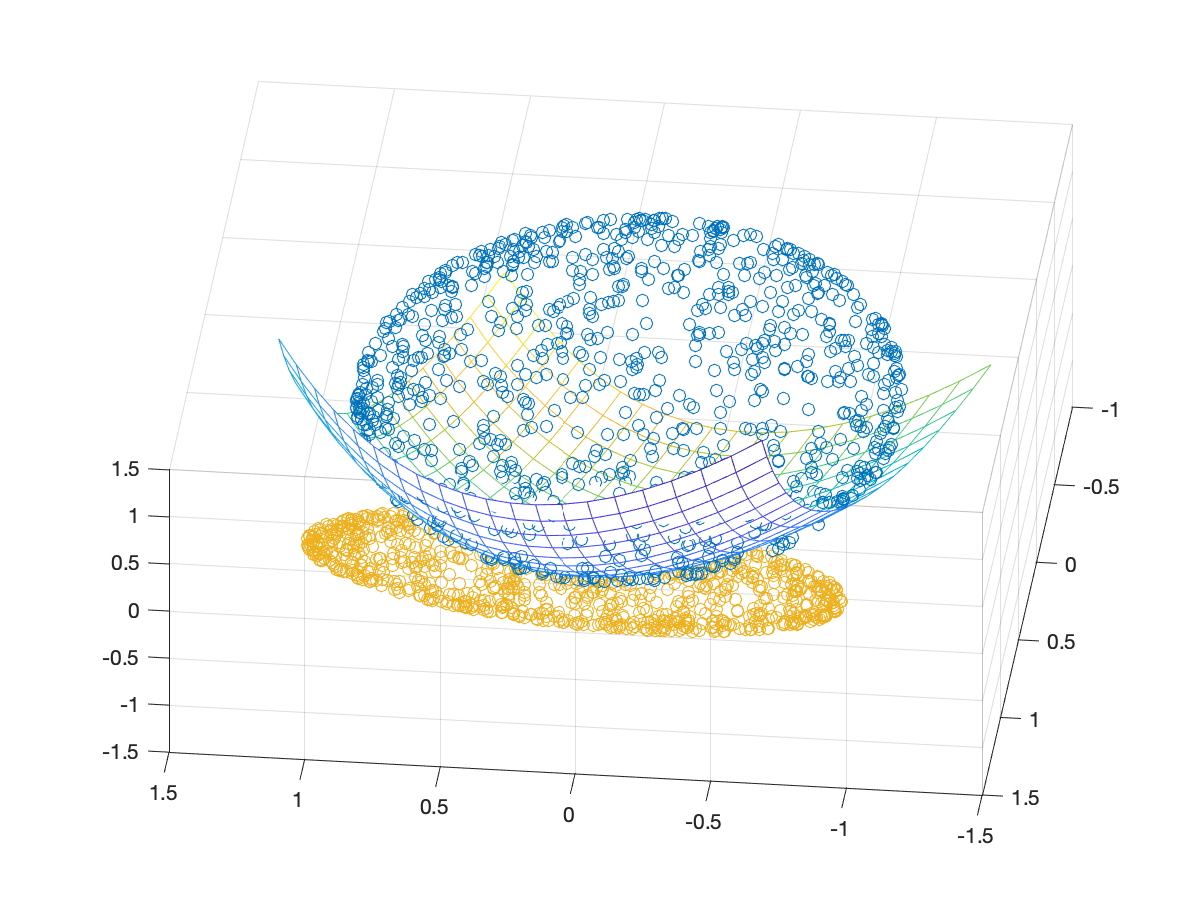
\includegraphics[width=2.5in]{demo.eps} 
   \caption{ Fitting a manifold with the elliptical paraboloid surface}
   \label{3-D paraboloid}
\end{figure}

%As shown in the Figure \eqref{3-D paraboloid}, the yellow circle $\circ$ is the projection of the points from the 3-dimensional ball onto the tangent space. The mesh surface is the fitted structure to locally approximate the manifold (3-dimensional ball). 
Obviously, from the Figure \ref{3-D paraboloid} we can see that the mesh surface is a better structure to approximate $\mathbb{S}^2$ compared with the tangent plane. Here,  the parameterized function of the quadratic form  $x_A(\tau): {\mathbbm R}^2\rightarrow {\mathbbm R}^3$ yields:
\[
x_A(\tau) = x_0 + U_{x_0} \tau + {U_{x_0}^\perp} \tau^T A \tau
\]
where $A$ is matrix of size $2\times 2$ which is used to control the shape and the direction of the paraboloid surface. The eigenvalues of $A$ represents the curvature or flatness in the corresponding eigenvector direction.
\end{example}
\remark{In 3-D space, obviously, 
when the paraboloid surface is at one side of the tangent plane, the matrix $A$ is positive definite or negative definite.
}
\subsection{Quadratic surface in high-dimensional space }

 Instead of fitting the manifold by the tangent plane, we bring a unknown function $\phi_{x_0}(\tau)$ from the tangent space to the normal space
 \[
 \phi_{x_0}(\tau): {\mathbbm R}^d \rightarrow {\mathbbm R}^{D-d}.
 \] 
 Using  $\phi_{x_0}(\tau)$, we know any manifold $\cal M$ locally at $x_0$ can be written as the range of  function   $x(\tau)$
  \begin{equation}\label{model}
  x (\tau)=  x_0 + U_{x_0} \tau+ U_{x_0}^{\perp} \phi_{x_0} (\tau),
  \end{equation}
where $\phi_{x_0}(\tau)=[\phi_{x_0}^{d+1}(\tau),...,\phi_{x_0}^{D}(\tau)]^T$  is the function from tangent space to the normal space. $\tau$ is the local coordinate in the tangent space.
From \eqref{model}, we know that there is a one-to-one correspondence between $\phi_{x_0} (\tau)$ and $x(\tau)$ as: %(equivalent to)
\begin{equation}\label{phi}
\phi_{x_0}(\tau) = {U_{x_0}^{\perp}}^{T}(x(\tau)-x_0)
\end{equation}
From \eqref{phi}, we know if we are given the structure of $\phi_{x_0}(\tau)$ with some parameters, we can have the representation of $\phi_{x_0}(\tau)$.
\begin{itemize}
\item[1,]  $x_0$ is any point on the manifold we are interested in.
\item[2,]  $U_{x_0}$ is the basis of principal space at $x_0$ which can be obtained from the local PCA. 
\item[3,]  $U_{x_0}^{\perp}$ is the orthogonal directions at $x_0$ which can also be obtained from the local PCA.
\item[4,]  The only remaining part is to  $\phi_{x_0} (\tau)$.
\end{itemize}

Note that, to implement the local PCA, the local covariance matrix at $x_0$ is defined as $C(x_0) = \sum_i K_h(x_0,x_i) (x_i-x_0)(x_i-x_0)^T$. The basis of the tangent space can be obtained from the eigenvalue decomposition as
\[
C(x_0) = [U_d , U_{D-d}] 
\left[
\begin{array}{cc}
\Lambda_1,& 0\\
0& \Lambda_2
\end{array}\right]
 [U_d , U_{D-d}]^T,
\]
in which from the decomposition, we can set $U_{x_0} = U_d, U_{x_0}^\perp = U_{D-d}$. In the local domain ${\mathbb R}_{x_0}^D (r)\cap \cal M$,  $\phi_x(\tau)$ can be approximated by the polynomial of order 2. Thus, we will get
\begin{equation}\label{app_phi}
\phi_{x_0}(\tau) = \phi_{x_0}(0)+ \nabla {\phi_{x_0}}(\tau)|_{\tau=0}(\tau)+ \frac{1}{2}{\nabla\nabla\phi_{x_0}(\tau)|_{\tau=0}}(\tau, \tau)+O(\|\tau\|_2^3)
\end{equation}
where ${\nabla\nabla\phi_{x_0}(\tau)|_{\tau=0}}$ stands for the second fundamental form which is a three order tensor with the size $ d\times d\times (D-d)$. Acting on $\tau$ twice will result in a vector of size $D-d$.  The linear operator  $\nabla {\phi_{x_0}}(\tau)|_{\tau=0}\in \mathbb{R}^{{(D-d)}\times d}$,  acting on $\tau$, will result in a vector size of $D-d$.

\begin{theorem}\label{tangent property}
If the columns of $U_{x_0}$ are the basis of tangent space of $\cal M$ at $x_0$, then, the nonlinear function $\phi_{x_0}(x)$ satisfies:
\[
\phi_{x_0}(0) = 0,\quad \nabla {\phi_{x_0}}(0) = 0.
\]
\end{theorem}
\begin{proof}
Recall that: $x (\tau)=  x_0 + U_{x_0} \tau+ U_{x_0}^{\perp} \phi_{x_0} (\tau)$. Let $\tau = 0$, then, we have
\[
U_{x_0}^{\perp} \phi_{x_0} (0) = 0
\]
Because of $U_{x_0}^{\perp}$ is a orthonormal matrix, $U_{x_0}^{\perp} \phi_{x_0} (0) = 0$ implies $\phi_{x_0} (0)=0$.

For any curve $\gamma(t)\in {\mathbbm R}^d, \gamma(0) = 0, \gamma'(0)=v$.
If we take the direction derivative for $x(\tau)$:
\[
\begin{aligned}
&\partial_v x(\tau)   = \frac{d x(\gamma(t))}{dt}|_{t=0} = \lim_{t\rightarrow 0} \frac{x(\tau+vt)-x(\tau)}{t}\\
=& \lim_{t\rightarrow 0} \frac{U_{x_0}(\tau+tv) -U_{x_0}(\tau)+U_{x_0}^{\perp} \phi_x(\tau+tv)-U_{x_0}^{\perp} \phi_x(\tau)}{t}\\
=&U_{x_0} v + U_{x_0}^{\perp} \nabla{\phi_x}(\tau) v
\end{aligned}
\]
Because  $\partial_v x(\tau)\in {\cal T}_{\cal M}({x_0})$, we have $U_{x_0}^{\perp} \nabla{\phi} (\tau)\in {\cal T}_{\cal M}({x_0})$.Thus, we have
\[
U_{x_0}^{\perp} \nabla {\phi} (\tau)= 0,
\]
which implies $ \nabla {\phi} (\tau)=0$ because the columns of the orthonormal matrix $U_{x_0}^{\perp}$ are linear independent .
\end{proof}
Because of Theorem \ref{tangent property}, recalling that \eqref{app_phi}, we know $\cal M$ can be parameterized with the remainder term:
\[
 x(\tau)= x_0+ U_{x_0} \tau + \frac{1}{2} U_{x_0}^{\perp}{\nabla\nabla\phi_{x_0}(\tau)|_{\tau=0}}(\tau, \tau)+O(\|\tau\|_2^3)
\]
For notational convenience, we denote the tensor as ${\cal A}_{x_0}=\frac{1}{2} {\nabla\nabla\phi_{x_0}(\tau)|_{\tau=0}}$ and define a new manifold ${\cal M_A}$ derived from $y_{\cal A}(\tau)$ as
\begin{equation}\label{M_a}
{\cal M_A} = \{ z| z =  x_0+ U_{x_0} \tau + U_{x_0}^{\perp} {\cal A}_{\phi_{x_0}}(\tau, \tau), \tau \in {\mathbb R}^d\}
\end{equation}
From \eqref{M_a}, we know ${\cal M_A}$ is derived from 
\[
y_{\cal A}(\tau) = x_0+ U_{x_0} \tau + U_{x_0}^{\perp} {\cal A}_{\phi_{x_0}}(\tau, \tau).
\]
Because of $y_{\cal A}(\tau)-x(\tau) = O(\|\tau\|_2^3)$, we know ${\cal M_A}$ approximates $\cal M$ well when $\tau_i$ is relatively small.
%\subsection{Paraboloid Surface}
%Define the paraboloid surface function at $x_0$ to be
%\begin{equation}\label{Paraboloid}
%\psi(\tau, {\cal A}_{\phi_{x_0}}) = x_0+ U_{x_0} \tau + U_{x_0}^{\perp} {\cal A}_{\phi_{x_0}}(\tau, \tau).
%\end{equation}
%We use it to fit manifold at a local domain of $R_{x_0}^D \cap \cal M$. From now on, if we don't need to emphasize the function $\phi_{x_0}$, we abbreviate ${\cal A}_{\phi_{x_0}}$ as $\cal A$ to represent the three order tensor.
\remark{
%Note, that the range of $\psi(\tau)$ is a quadric approximation of manifold $\cal M$. 
In most of the manifold fitting cases, both of the true manifold $\cal M$ and the function $\phi_{x_0}(\tau)$ are unknown, as a result, it is impossible for us to get the second order parameter ${\cal A}_{x_0}$ through differentiate $\phi_{x_0}(\tau)$.

 Instead of get the accurate $\phi_{x_0}(\tau)$, we can estimated it by using the data (observations) which is supposed to be drawn from some low-dimensional manifold. In this case, we need to estimate the ${\cal A}_{\phi_{x_0}}$ from the observations to obtain $\hat{\cal A}$, as a result, the range $y_{\hat{\cal A}}(\tau)$ can be assumed a local smoothed approximation of $\cal M$ around $x_0$ to some degree.
}

From now on, we will abbreviate $\hat{\cal A}$ as ${\cal A}$, to stand for the estimated second order parameter.
\subsection{Fitting Model}

In real case, when we have samples from the manifold, we need to determine  $U_{x_0}, {\cal A}_{\phi_{x_0}}(0)$ by knowing $x_0, \{x_i\}$.

Using local principal analysis, we know for each observation $x_i$, there is a local coordinate $\tau_i = \tau(x_i,x_0, U_{x_0})$ in the tangent space. When we use $x_0$ as the origin of the coordinate. By projecting onto the tangent space, we have the local coordinate has the closed-form solution as
\begin{equation}\label{tangent_coor}
\tau_i = U_{x_0}^T (x_i -x_0).
\end{equation}
When having $\{\tau_i, U_{x_0}, x_0\}$, we can determine the tensor $\cal A$ by a least square problem. The global coordinate $x_i$ has a second order approximation as
\begin{equation}\label{x_tau}
 x_i  -  (x_0+ U_{x_0} \tau_i + U_{x_0}^{\perp} {\cal A}(\tau_i,\tau_i)) = o(\|\tau_i\|_2^2).
\end{equation}
%where we can split the tensor acting on $\tau_i$ as
%\[
%{\cal A}_{\phi_{x_0}}(0)(\tau_i,\tau_i) = [\tau_i^T S^{d+1}\tau_i, ...,\tau_i^T S^{D}\tau_i]^T.
%\]
We should find a tensor $\cal A$ such that the remainder is a higher order item.
%\begin{equation}\label{optimA}
% \|x_i  -  (x_0+ U_{x_0} \tau_i + U_{x_0}^{\perp} {\cal A}(\tau_i,\tau_i)) \|_2^2
%\end{equation}
Substitute \eqref{tangent_coor}, into \eqref{x_tau}, we have
\[
 x_i  -  (x_0+ U_{x_0} \tau_i + U_{x_0}^{\perp} {\cal A}(\tau_i,\tau_i))
 =U_{x_0}^\perp( {U_{x_0}^\perp}^T (x_i -x_0) -{\cal A}(\tau_i,\tau_i) )= o(\|\tau_i\|_2^2)
\]
which is equivalent to 
\begin{equation}\label{normal_appro}
 {U_{x_0}^\perp}^T (x_i -x_0) -{\cal A}(\tau_i,\tau_i) = o(\|\tau_i\|_2^2)
\end{equation}
%For \eqref{phi}, we can get the best estimated value of ${\cal A}_{\phi_{x_0}}(0)(\tau_i,\tau_i) $ as
%\begin{equation}\label{all-dimension}
%{U_{x_0}^\perp}^T (x_i -x_0)  = \hat{\cal A}_{\phi_{x_0}}(0)(\tau_i,\tau_i)  + o(\|\tau_i\|_2^2)
%\end{equation}
Noticing that \eqref{normal_appro} is a vector form, split \eqref{normal_appro} into each dimension, e.g, for the $k$-th dimension in the normal space, we have
\begin{equation}\label{normal_approx}
 {(u^k_{x_0})}^T (x_i -x_0) 
={\cal A}_{\cdot\cdot k}(\tau_i,\tau_i) +  o(\|\tau_i\|_2^2)=\tau_i^T S^{k}\tau_i + o(\|\tau_i\|_2^2)\end{equation}
In \eqref{normal_approx}, because of the symmetric position of $\tau_i$, we know that the best fitted $S^k$ is symmetric, i.e, each slice of ${\cal A}_{\cdot\cdot k}$ is a symmetric matrix. Therefore, the unknown parameters in $S^k$ yields a total number of ${d(d+1)}/{2}$. 

In \eqref{normal_approx}, the only unknown is $\cal A$, finding the best approximation of $\cal A$ in the $\|\cdot\|_2^2$ criteria is a linear regression or least square problem. To use the linear algebra tools, we should vectorize each slice of $\cal A$.

In the following section, we will show how to vectorize each slice of $\cal A$ and  how to make the vectorized result into the matrix form. Also, we show the quadratic form equals to the inner product of two vectors as
\[
\tau_i^T S^{k}\tau_i  = 2{\rm vech}(\tau_i\tau_i^T,1)^T {\rm vech}(S^k,1/2)
\]

\subsection{Closed-form of $S^k$ by Vectorization}
In this section, we vectorize the matrix, such that we could obtain $S^k$ by using a least square problem with samples $\{x_i\}$.

For any symmetric matrix $A$, we know $A_{ij} = A_{ji}$. Therefore, we can only need ${d(d+1)}/{2}$ elements with the corresponding order to restore it. As a result, we can only vectorize the upper-triangle elements in the matrix $A$ as a vector 
\[
{\rm vech}(A,t)_{\frac{(2d-i)(i-1)}{2}+j-i+1} = \left\{
\begin{array}{cc}
A_{ij},    &\quad j>i\\
tA_{ij},&\quad j=i
\end{array}
\right.
\]
where the diagonal elements multiplied by a scalar $t$, which will bring us convenience for our following notations. When $t=1$, the vector is constructed by picking the upper-triangle elements of $A$ including the diagonal ones, i.e., 
\[
{\rm vech}(A,1) = [A_{11},A_{12},...A_{1d},...A_{dd}]^T.
\]
When $t=1/2$, the vector is constructed by picking the upper-triangle elements of $A$, and half of the diagonal elements, i.e.,
\[
{\rm vech}(A,{1}/{2}) = [A_{11}/2,A_{12},...A_{1d},...A_{dd}/2]^T.
\]
%Here, the vectorization operates with the elements in ${\rm vech}(A,1)$ and $A$ yield a relation as:
%\begin{gather*}
%{\rm vech}(A,1)_{\frac{(2n-i)(i-1)}{2}+j-i+1} = \left\{
%\begin{array}{cc}
%A_{ij},    &\quad j>i\\
% A_{ij},&\quad j=i
%\end{array}
%\right.\\
%{\rm vech}(A,1/2)_{\frac{(2n-i)(i-1)}{2}+j-i+1} = \left\{
%\begin{array}{cc}
%A_{ij},    &\quad j>i\\
% A_{ij}/2,&\quad j=i
%\end{array}
%\right.
%\end{gather*}
%Notice that $\theta_k$ is obtained by selecting the upper-triangle elements of $S^k$. 
Note that, we can easily recover the matrix $A$ from the vector ${\rm vech}(A,1/2)$ by
%Conversely, we can also recover $S^k$ from $\theta_k$, by
\[
A = {\rm Mat} ({\rm vech}(A,1/2)) + {\rm Mat}^T ({\rm vech}(A,1/2)) 
\]
where ${\rm Mat}(y)$ is an operator constructed by realigning the elements in $y$ into a upper-triangle matrix ${\rm Mat} (y)$ such that the $i,j$-th elements equals
\[
{\rm Mat} (y) _{i,j} =\left\{
\begin{array}{cc}
 y_{{(2d-i)(i-1)}/{2}+j-i+1},& j\geq i\\
 0,& j<i
\end{array}
 \right.
\]
With the above notations, the quadratic form $x^T A x$ can be written in the vectorized version as
\[
x^T A x = 2{\rm vech}(xx^T,1)^T {\rm vech}(A,1/2)
\]
where ${\rm vech}(xx^T,1)$ is a vectorization of the symmetric matrix $xx^T$ including the diagonal ones.
\remark{
The vectorization process for a symmetric matrix is invertible, i.e, if we vectorize a symmetric matrix into a vector, we can also turn the vector into a matrix which is identical with the former one.
}



%We can vectorize the matrix $\tau_i \tau_i^T$ by placing the upper-triangle of elements in $\tau_i \tau_i^T$ into a vector $g_i$ by
%\[
%g_i  =  [{\tau_i}_{1}^2, {\tau_i}_{1}{\tau_i}_{2},...,{\tau_i}_d^2]^T, 
%\]

%For notational convenience, we denote $\theta_k = {\rm vech}(S^k)$. 
Because of the symmetric of the matrix $\tau_i\tau_i^T$ and $S^k$, using the above notations, it can be easily verified that
\[
\tau_i^TS^k\tau_i = \langle \tau_i\tau_i^T, S^k\rangle =2{\rm vech}(\tau_i\tau_i^T,1)^T {\rm vech}(S^k,1/2)%= 2 \theta_k^T g_i
\]
For notational convenience, we denote $\theta_k = {\rm vech}(S^k,1/2)$ and $g_i = {\rm vech}(\tau_i\tau_i^T,1)$.
Using the vector notations, the equation in \eqref{normal_approx} can be converted as:
\begin{equation}\label{g_i}
g_i^T \theta_k  - \frac{1}{2}{(u^k_{x_0})}^T (x_i -x_0) = o(\|\tau_i\|_2^2).
\end{equation}
For notational convenience, we use $z_i^k$ to stand for the local coordinate in the $k$-th normal dimension corresponding to $x_i$, i.e.,
\[
z_i^k =  \frac{1}{2}{(u^k_{x_0})}^T (x_i -x_0) %+ o(\|\tau_i\|_2^2).
\] 
From \eqref{g_i}, we know that
\[
g_i^T \theta_k  - z_i^k= o(\|\tau_i\|_2^2).
\]
To determine the ${d(d+1)}/{2}$ parameters in $\theta_k$, we need ${d(d+1)}/{2}$ linear independent equations. In other words, we need at least ${d(d+1)}/{2}$ samples to construct ${d(d+1)}/{2}$ linear independent $\{g_i, i = 1,...,{d(d+1)}/{2}\}$. 

Suppose, we have $m$ samples on the manifold. Denote the matrix $G$ and the vector $\ell_k$ as
\[
G = [g_1,...,g_m]^T, \quad \ell_k = [z_1^k,..., z^k_m ]^T.
\]
\remark{ Idealy, we only need ${d(d+1)}/{2}$ samples to fix $\{S^k,k=d+1,D\}$ if and only if the rows of $G$ can span the whole space of the ${{d(d+1)}/{2}}$-dimensional space, i.e. ${\rm rank}(G)={d(d+1)}/{2}$. If we have less than ${d(d+1)}/{2}$ samples, we have multiple choice for each of the $S^k$ in $\{S^k,k=d+1,...,D\}$.
}
\subsection{Sample Related Weights}
Using the samples to estimate $\theta_k$ in \eqref{g_i}, it should be noted that we want a locally fitting model, which means we want ${\cal M_A}$ be defined as the range of $x_{\cal A}(\tau)$
\begin{equation}\label{M_A}
{\cal M_A} = \{x:x_{\cal A}(\tau) = U_{\perp} {\cal A} (\tau,\tau) + U \tau +x_0,\tau\in {\mathbb R}^d\},
\end{equation}
to fit $\cal M$ well when $\|\tau\|_2$ is relatively small. To achieve this goal, the points which reside nearby $x_0$ should have a larger weight.
Then, by using a nonlinear kernel function $K_h(\cdot)$, the optimal minimization problem with respect to the $k$-th dimension becomes
\begin{equation}\label{optimal}
  \min_{\theta_k} \sum_{i=1}^m K_h(x_i-x_0)\{ g_i^T \theta_k  - \frac{1}{2} {(u^k_{x_0})}^T (x_i -x_0)\}^2
= \|W_h^{1/2}(G \theta_k-\ell_k) \|_2^2,
\end{equation}
where $W_h$ is a diagonal matrix and the $i$-th element is $\{{W_h}\}_{ii} = K_h(x_i-x)$. Denote the column space ${\cal C} = {\rm span}\{ W_h^{1/2}G_1, ...,W_h^{1/2}G_{{d(d+1)}/{2}}\}$
\begin{equation}\label{fit_obj}
\|W_h^{1/2}(G \theta_k-\ell_k) \|_2^2 =\underbrace{ \|W_h^{1/2}G \theta_k - P_{\cal C} (W_h^{1/2}\ell_k)\|_2^2}_{(e.1)}+\underbrace{\|P^{\perp}_{\cal C} (W_h^{1/2}\ell_k)\|_2^2}_{(e.2)}
\end{equation}
\remark{
The term $(e.1)$ determines whether we have multiple choice of parameters corresponding the form of $x(\tau)$ which could yields the same least approximation error.  The second term $(e.2)$ indicates whether $x(\tau)$ can go through the samples, if  the term $(e.2)$ equals zero, we can infer that we can have $x(\tau)$ go through the samples exactly.
}
\subsection{Solution Behavior for $S^k$(or $\theta_k$)}
The behavior of $\psi(\tau)$ can be observed from the two parts in \eqref{fit_obj} as
\subsubsection*{Case \romannumeral1: $\|P^{\perp}_{\cal C} (W_h^{1/2}\ell_k)\|_2^2=0$}
By evaluating $\|P^{\perp}_{\cal C} (W_h^{1/2}\ell_k)\|_2^2$, we can confirm whether $\psi(\tau)$ can go through the $m$ samples. If $\|P^{\perp}_{\cal C} (W_h^{1/2}\ell_k)\|_2^2=0$, the minimum value of the problem \eqref{optimal} is zeros which implies $\phi_{\cal A}(\tau)$ pass the $m$ samples on the manifold.
\subsubsection*{Case \romannumeral2: ${\rm rank}(G)={d(d+1)}/{2}$ } 
The column-rank equals to the rank of $G$. If there is ${\rm rank}(G)={d(d+1)}/{2}$, then, we know the columns of $G$ are linear independent. Since $W^{1/2}_h$ is a full-rank matrix, the linear independent of $G$ implies the linear independent of $W^{1/2}_hG$. As a consequence,  there is a unique representation of $P_{\cal C} (W_h^{1/2}\ell_k)$ in the space spanned by the columns of $W_h^{1/2} G$, which is the parameter $\theta_k$ in \eqref{fit_obj}. The unique solution of \eqref{optimal} is
\begin{equation}\label{solution}
\hat{\theta}_k = (G^TW_hG)^{-1} G^T W_h^{1/2} P_{\cal C} (W_h^{1/2}\ell_k)
\end{equation}
Because there is an one-to-one corresponding between $\hat{S}^k$ and $\hat{\theta}_k$, the uniqueness solution of $\hat{\theta}_k$ implies we have a unique $\hat{S}^k$.
\subsubsection*{Case \romannumeral 3: ${\rm rank}(G)<{d(d+1)}/{2}$ } 
 The rank of $G$ equals the column rank of $W_h^{1/2}G$ because $W_h^{1/2}$ is a full rank matrix.  As a result, ${\rm rank}(G)<{d(d+1)}/{2}$ implies the columns of $W_h^{1/2}G$ are linear dependent. Therefore, the linear system 
 \begin{equation}\label{linear_system}
 W_h^{1/2}G \alpha = 0,
 \end{equation}
 has nonzero solutions. Since the dimension of the space $\cal Q$ spanned by the rows of $W_h^{1/2}G$ is ${\rm rank}(G)$, any vector in the orthogonal space  ${\cal Q}^{\perp}$ is the solution of the linear system \eqref{linear_system}. Thus, in this case, $\hat{\theta}_k$ has multiple solutions, which can be written as:
 \[
 \hat{\theta}_k =  \tilde{\theta}_k + \sum_{u=1}^{r} c_r e_r
 \]
 where $r = {d(d+1)}/{2}-{\rm rank}(G)$, $\{c_r\}$ is any nonzero parameter and $\{e_r\}$ is the basis of the subspace of ${\cal Q}^{\perp}$. $\tilde{\theta}_k$ is any special solution for the linear system
 \[
 W_h^{1/2}G \theta_k  = P_{\cal C} (W_h^{1/2}\ell_k).
 \]
 Because $P_{\cal C} (W_h^{1/2}\ell_k)$ is in the column space of $W_h^{1/2}G$, it is certain that there is some $\tilde{\theta}_k$ can satisfy the above equation.
 \subsection{Perturbation Analysis}

 In the above discussion, we assume $x_0$ is some point on the manifold. In real manifold fitting cases, we only have data points $\{x_i\}$ and some outlier $x$ with we want to project onto the underline manifold $\cal M$. The process to estimate $x_0$ from $x$ will be discussed in section
 \ref{Origin Point Selection}.  
%First, we assume:
% Define 
% \[
% F(x_0) = \sum_i K_h(x,x_i) (x_i-x_0)(x_i-x_0)^T
% \]
%  \begin{assumption}
% The estimation error $e_0$ in $x_0$ is small enough, such that the eigenspaces $U_d, \tilde{U}_d$  of the two matrices $F(x_0), F(\tilde{x}_0)$ yields
% \[
% \|U_dU_d^T -  \tilde{U}_d\tilde{U}_d^T\| = O(F(x_0) - F(\tilde{x}_0)) = o(\|e_0\|_2^2)
% \]
% \end{assumption}
In the construction of $\{U, U_\perp\}$ only depending on the outlier $\bar{x}$ and the observation $\{x_i\}$.
 
 As a result, we know $x_0$ can not be exactly on $\cal M$. Suppose the estimated $x_0$ be written as
 \[
 x_0 = \tilde{x}_0 +e_0 
 \]
 where $\tilde{x}_0$ is the projection of $x_0$ onto $\cal M$ and $e_0$ is the approximation error in the normal space ${\cal N}_{\cal M}(\tilde{x}_0)$. The real relationship of \eqref{normal_approx} should be:
 \begin{equation}\label{zki1}
 \tilde{z}_i^k =  {(u^k)}^T (x_i -\tilde{x}_0) 
={\cal A}_{\cdot\cdot k}(\tau_i,\tau_i) +  o(\|\tau_i\|_2^2)%=\tau_i^T S^{k}\tau_i + o(\|\tau_i\|_2^2)
 \end{equation}
However, because of the unknown $\tilde{x}_0$, we approximate through the relation
\begin{equation}\label{zki2}
 z_i^k =  {(u^k)}^T (x_i -{x}_0) = {\cal A}_{\cdot\cdot k}(\tau_i,\tau_i)+  o(\|\tau_i\|_2^2)
\end{equation}
Because of \eqref{zki1} and \eqref{zki2}, we have the error is not related with the $i$-th sample, i.e,
\[
 \tilde{z}_i^k -z_i^k = (u^k)^T e_0.
\]
 Recalling the definition of $\ell_k$,  we have the true $\tilde{\ell}_k = [\tilde{z}_1^k,...,\tilde{z}_m^k]$ and the $\ell_k=[z_1^k,...,z_m^k]$ has a relation as
 \[
 \tilde{\ell}_k = \ell_k + (u^k)^T e_0 {\mathbbm{1}}.
 \]
 The stability for the solutions corresponding to the two linear systems  with respect to$\ell_k$ and $\tilde{\ell}_k$ is highly related with the condition number of $G^T W_h G$
 \[
 W_h^{1/2}G \tilde{\theta}_k  =  P_{\cal C} (W_h^{1/2}\tilde{\ell}_k);\quad W_h^{1/2}G \theta_k  =  P_{\cal C} (W_h^{1/2}\ell_k).
 \]
 The error is
 \[
 \tilde{\theta}_k -\theta_k = (G^T W_h G)^{-1} G^T W_h^{1/2} P_{\cal C} ( W_h^{1/2}u^k e_0 {\mathbbm{1}}).
 \]
\subsection{Geometric Interpretation of $S^k$}
Since $S^k$ is a symmetric matrix, its eigenvalues all exist in real field. Here, we will show the definite property of $S^k$ determines the shape of our fitted function.  It is natural that we can give an analysis depending on the definite property of $S^k$.
\subsubsection*{Case \romannumeral1: positive (or negative) definite $S^k$}
Note that, in our quadratic function of \eqref{M_A},  the positive-define property of $k$-th slice $S^k$ of $\cal A$ indicates that the quadratic term of the $k$th component satisfies for all $\tau\in {\mathbb R}^d$
\[
\tau^T S^k\tau \geq 0.
\]
Furthermore, if each of the slice $S^k$ in $\cal M_A$ is positive-definite, we can conclude that our quadratic surface ${\cal M_A}$ resides only on one side of the tangent plane $\{x|x=U_d\tau+x_0\}$.
\subsubsection*{Case \romannumeral2: indefinite $S^k$}

Recall that in 3-dimensional space, the function of a saddle surface go through $(0,0,0)$ yields a form as
\[
(x,y,z) =( \tau_1, \tau_2, {\tau_1^2}/{a}+{\tau_2^2}/{b}),
\]
where $ab<0$. Denote $\tau = (\tau_1,\tau_2)$. When we rotate the coordinate with an orthogonal matrix $[U,U_\perp]$ and move the origin $(0,0)$ to $x_0$, the above parametric function becomes
\[
 (x(\tau),y(\tau),z(\tau)) = U\tau+U_\perp (\tau^T 
 \left[
 \begin{array}{cc}
 a,&0\\
 0,&b
 \end{array}
 \right]
 \tau)
 +x_0.
\]
Note that, in this case, the second order parameter $A =  \left[
 \begin{array}{cc}
 a,&0\\
 0,&b
 \end{array}
 \right]$ is an indefinite matrix because of $ab<0$. 
 
\begin{figure}[t] %  figure placement: here, top, bottom, or page
   \centering
   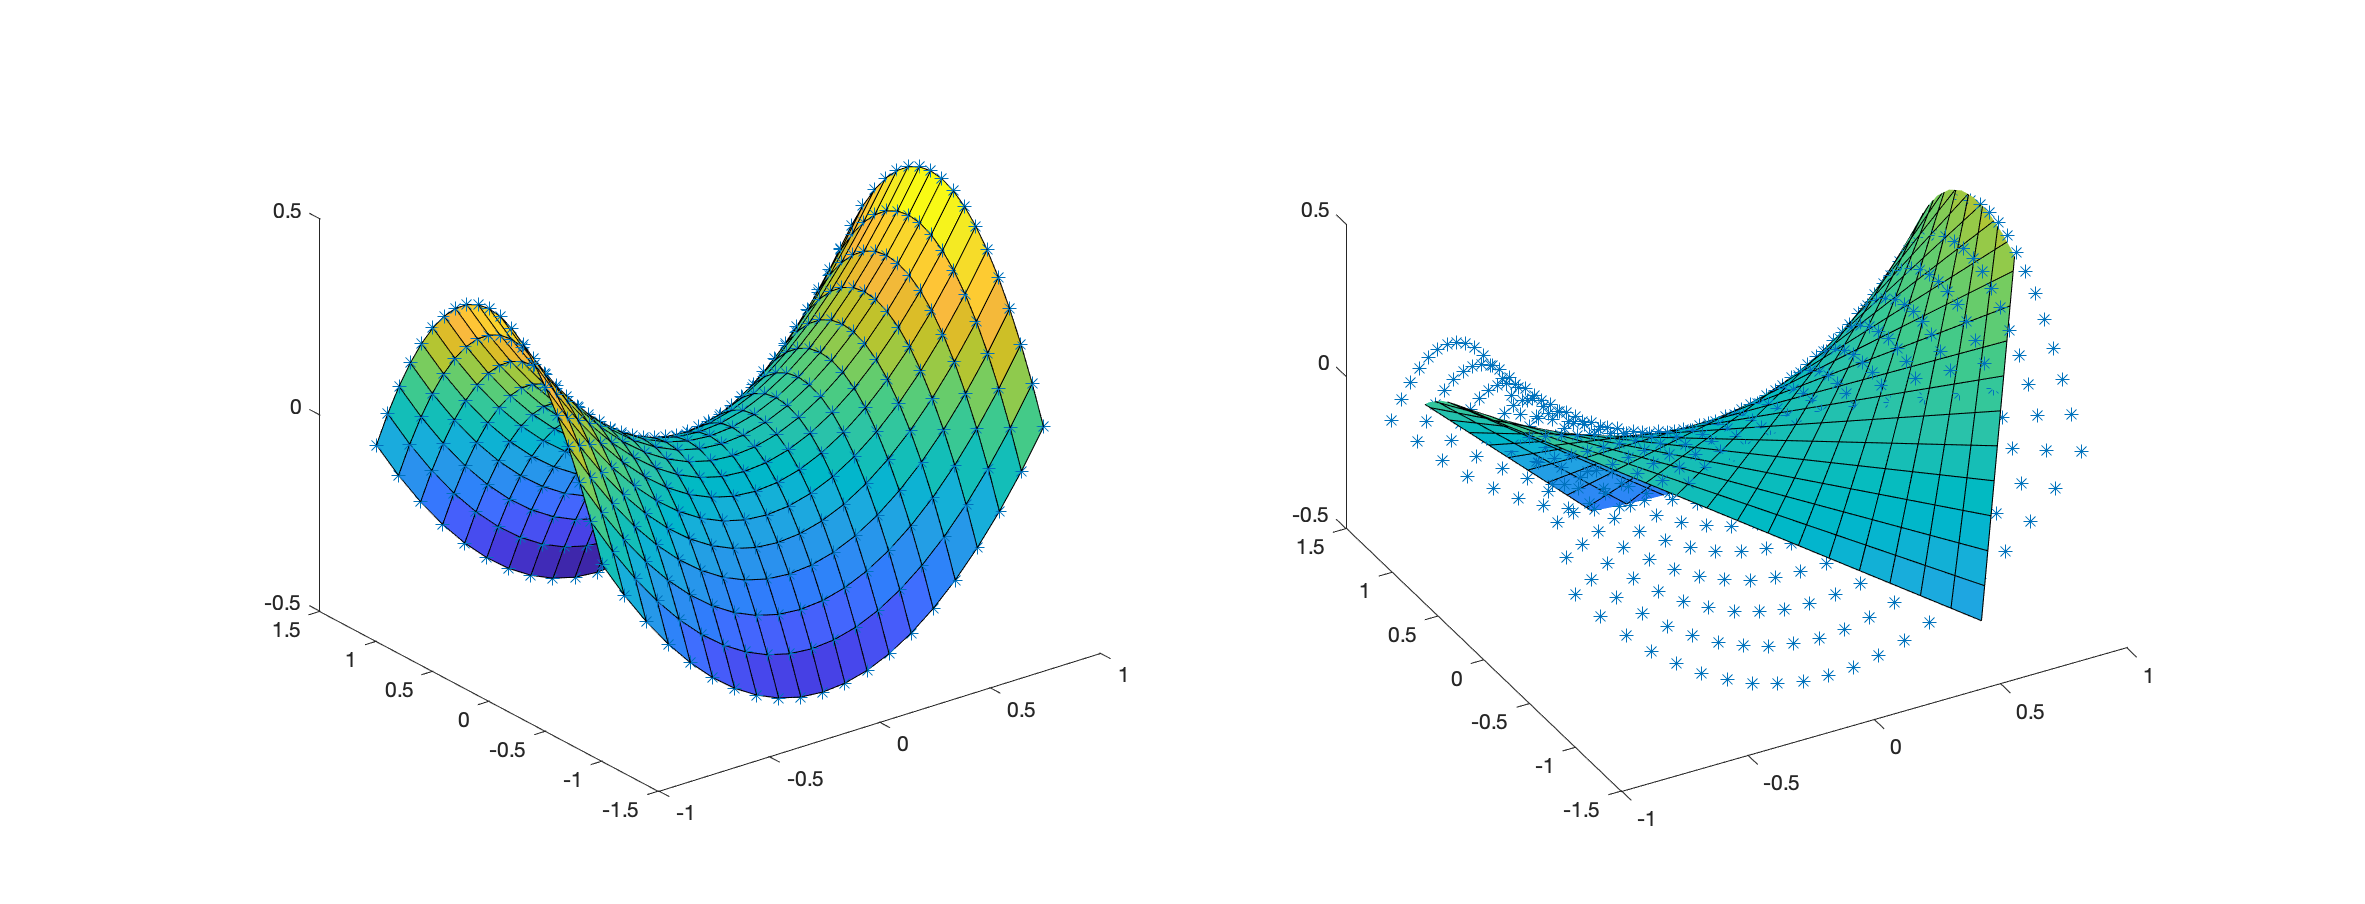
\includegraphics[width=\linewidth]{saddle.eps} 
   \caption{Illustration of hyperbolic  fitting case: Left: fitting at $(0,0,0)$, Right: fitting at $(1/2,1/2,0)$. Data drawn from function $(x,y,z) = (\tau_1,\tau_2, {\tau_1^2}/{2}-{\tau_2^2}/{2})$ without distrurbed by noise:  }
   \label{fig:example}
\end{figure}
 
 For general case in higher dimension,  an indefinite matrix $S^k$ will result in a  hyperbolic paraboloid in the corresponding dimension $k$ in normal space. Suppose $S^k$ yields a eigen-decomposition of the form
 \[
 S^k = [V_1,V_2]
 \left[
 \begin{array}{cc}
 \Lambda_1&0\\
 0&\Lambda_2
 \end{array}
 \right]
 [V_1,V_2]^T
 \]
 where the diagonal elements  of $\Lambda_1$ are positive, and diagonal ones of $\Lambda_2$ are negative. Thus, we know the space spanned by the columns of $U_\perp V_1$ is second order positive, i.e., any direction restricted in this space is a subspace-restricted local minimum point. Conversely,  the space spanned by the columns of $U_\perp V_2$ is second order negative, i.e., any direction restricted in this space is a subspace-restricted local maximum point. Thus, recalling that the second order surface is tangent to the first-order plane $\{x(\tau) |x(\tau)=x_0+U\tau\}$ at $x=x_0$, the origin point $x_0$ is a saddle point.
 
 In our manifold fitting problem, because we do not has any prior information on the manifold besides the observations, we do not restrict $S^k$ to be a positive (or negative) matrix. The definite (or indefinite) property is decided by our fitting model and the inputed data.

%In this case, we have multiple choice of $S_k$ given the current observations. Any of the $S_k$ is the optimal solution for the 2-order fitting problem.
%\subsection{Solution}
%Depending on difference of the shape and the rank of $G$, we have the following cases:
%\subsubsection*{Case \romannumeral1: $m=\frac{d(d+1)}{2}$, ${\rm rank}(G) = \frac{d(d+1)}{2}$}
%In this case, \eqref{g_i} can be written as
%\[
%G  (vec({\rm Triu}(S^k))) = \ell_k
%\]
%Thus, $G$ is invertible, the closed-form of $vec({\rm Triu}(S^k))$ can be written as
%\[
%vec({\rm Triu}(S^k))  = {G}^{-1} \ell^k
%\]
%\remark{ Here, we can build $\psi(\tau)$ to go through all the $\frac{d(d+1)}{2}$ samples.
%}
%\subsubsection*{Case \romannumeral2: $m>\frac{d(d+1)}{2}$, ${\rm rank}(G) > \frac{d(d+1)}{2}$}
%
%\remark{ There are $d\times d$ parameters in $S^{k}$
%}
\subsection{Asymptotic Properties}
In this section, we give the asymptotic properties of our fitted $\hat{S}^k$ and the true $S^k$ (Hessian of $\phi_k(\tau)$ at $0$) with the behaviors of $n$ and $h$.
\begin{theorem}
For the estimated $\hat{\theta}_k$, the error between $\hat{\theta}_k$ and the true $\theta_k$ is with the order of 
\[
\hat{\theta}_k - \theta_k = O(h) +O_p(\frac{1}{\sqrt{nh^{D-2}}})
\] 
where $n$ is the number of observations and $h$ is the bandwidth selected in our locally least square problem.
\end{theorem}
\begin{remark}
Obviously, the optimum order of $h$ is $h=O(\frac{1}{n^{1/D}})$.  With the increasing of observations, we could choose a relatively small $h$ such that the estimated error is relatively small.
\end{remark}

\section{Manifold Fitting via Nonlinear Projection}
In this section, we show how to implement a nonlinear projection onto our fitted manifold, also give some theoretical result to ensure the convergence properties.

\begin{figure}[t] %  figure placement: here, top, bottom, or page
   \centering
   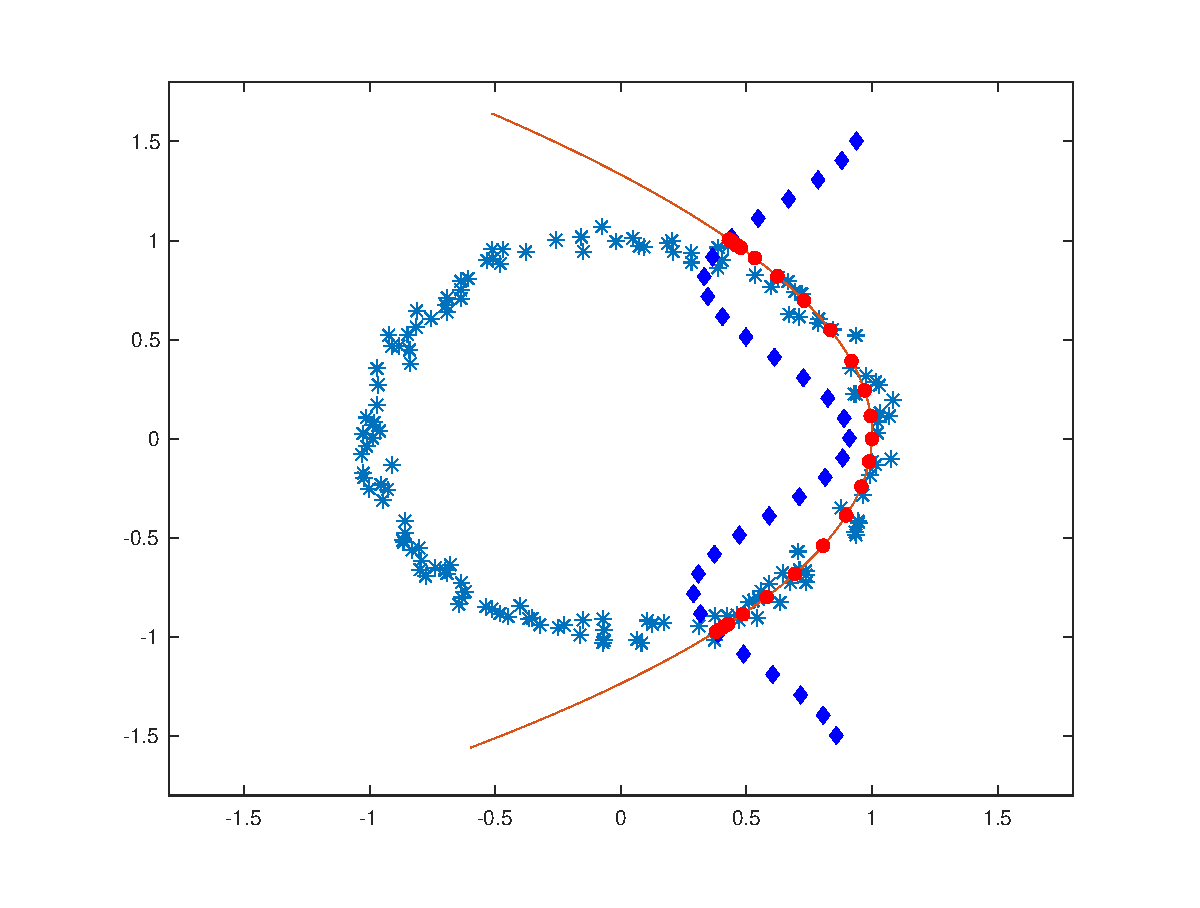
\includegraphics[width=0.6\linewidth]{demo3.eps} 
   %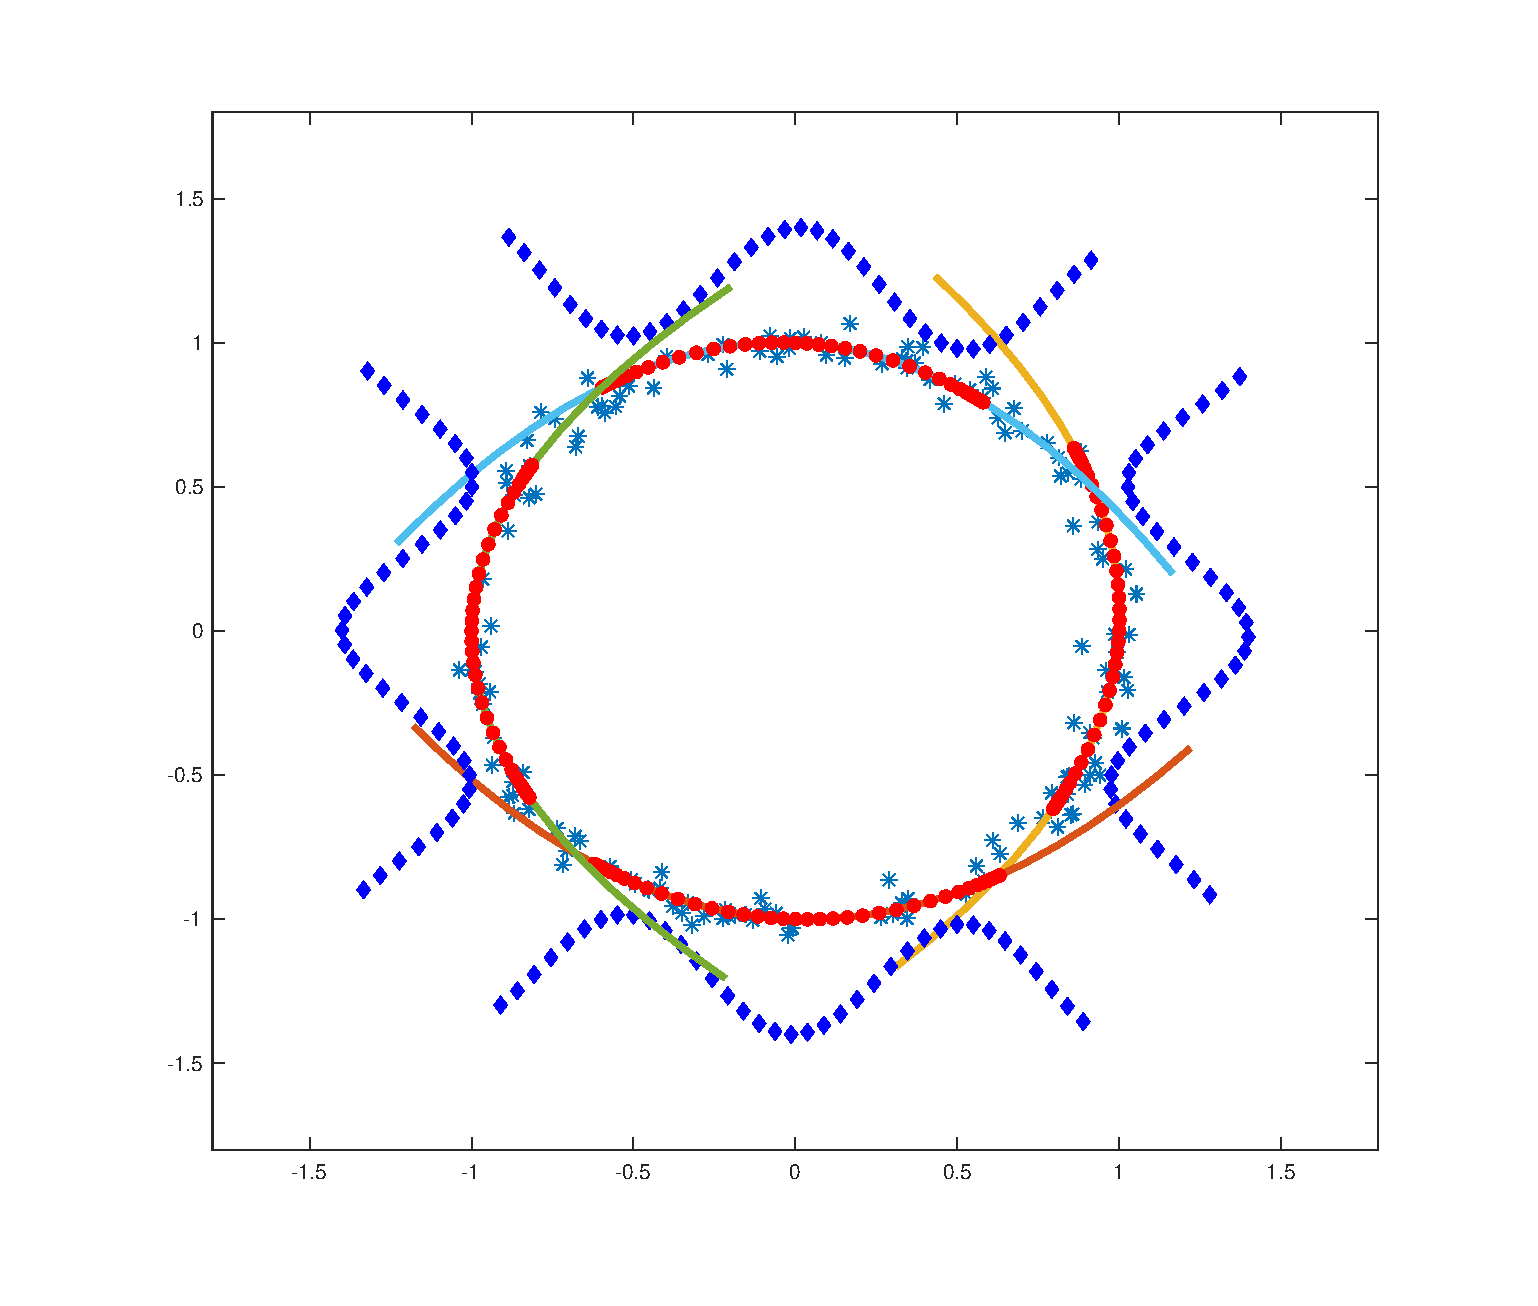
\includegraphics[width=0.48\linewidth]{fit_demo.eps} 
   \caption{Demo for Nonlinear Projection }
   \label{fig:example}
\end{figure}

The manifold fitting problem can be viewed as projecting data $x$ to a local approximated structure. The works before considers this local structure as an affine plane (parameter with $\tau$), such as
\[
 x(\tau)  =  U \tau +x_0
\]
In our work, we can have a fitted paraboloid surface, with the form of a quadratic form as
\begin{equation}\label{manifold_representation}
x_{\cal A}(\tau) = U_{\perp} {\cal A} (\tau,\tau) + U \tau +x_0
\end{equation}
where $x_0$ is the origin (center for the local coordinate).

\subsection{Projection onto Manifold}
Suppose we have a locally fitted manifold which has the parameterized form written as $x(\tau): {\mathbb R}^d\rightarrow {\mathbb R}^D$.
Since the range of the function $x_{\cal A}(\tau)$ generated a simple manifold, we denote it as 
\[
{\cal M}_{\cal A} = \{y: y = x_{\cal A}(\tau), \tau\in {\mathbb R}^d\}.
\]
Given any $z\not\in{\cal M}_{\cal A}$, we define the projection $P_{{\cal M}_{\cal A}}(z)$  of $z$ onto ${\cal M}_{\cal A}$ as
\begin{equation}\label{projection}
P_{{\cal M}_{\cal A}}(z) = \arg\min_{w \in {\cal M}_{\cal A} }\|w-z\|_2.
\end{equation}
Using the function $x_{\cal A}(\tau)$, we know the points on ${\cal M}_{\cal A}$ and the Euclidean space $R^d$ is one-to-one. As a result, instead of find $w$, in \eqref{projection}, we just need to find $\tau$
\begin{equation}\label{projection_tau}
 \hat{\tau} = \arg\min_{\tau\in R^d }\|z-x_{\cal A}(\tau)\|_2^2.
\end{equation}
Finally, using the explicit form $x_{\cal A}(\tau)$, we know
\[
P_{{\cal M}_{\cal A}}(z) = x_{\cal A}(\hat{\tau})=x(\arg\min_{\tau\in R^d }\|z-x_{\cal A}(\tau)\|_2^2).
\]
\remark{ 
In \eqref{projection_tau}, we minimize the squared of 2-norm instead of 2-norm for two reasons. First, optimizing with respect to $\|\cdot\|_2^2$ and $\|\cdot\|_2$ is equivalent because of $f^2(x)$ and $f(x)$ share the same monotonous property in the intervals of $\{x|f(x)>0\}$. Second, $\|\cdot\|_2^2$ is a polynomial, which has easier form with respect to derivatives for any order.
}

Overall, the projection onto ${\cal M}_{\cal A}$ consists of the following two steps:
\begin{itemize}
\item[1.] Solve the nonlinear problem: Given $z$, find $\tau$ such as 
\begin{equation}\label{nonlinear_projection}
\hat{\tau} = \min_\tau \|z -  (U_{\perp} {\cal A} (\tau,\tau) + U \tau +x_0)\|_2^2
\end{equation}
\item[2.] Construct the coordinate in the ambient space
\[
\hat{z} = U_{\perp} {\cal A} (\hat{\tau},\hat{\tau}) + U \hat{\tau} +x_0
\]
\end{itemize}
To solve the nonlinear projection problem \eqref{nonlinear_projection}, we can simplify it as
\begin{equation}\label{simiplified_nonlinear}
\begin{aligned}
   &\|z -  (U_{\perp} {\cal A} (\tau,\tau) + U \tau +x_0)\|_2^2\\
 =&\|P_U(z-x_0)-U\tau\|_2^2+\|P_{U_{\perp}}(z-x_0)-(U_{\perp} {\cal A}(\tau,\tau))\|_2^2 \\
  =&\|U (U^T (z-x_0)-\tau)\|_2^2+\|U_\perp (U_{\perp}^T(z-x_0)- {\cal A}(\tau,\tau))\|_2^2 \\
 =&\|U^T (z-x_0)-\tau\|_2^2+\|U^T_{\perp}(z-x_0)- {\cal A} (\tau,\tau)\|_2^2
\end{aligned}
\end{equation}
\remark{
The optimization problem in \eqref{simiplified_nonlinear} is nonlinear, with the highest order term corresponding to $\tau$ is quartic. As far as we know, there is no closed-form solution to directly minimize \eqref{simiplified_nonlinear}. The difficulty originates from the relatively higher order. If we can decrease the order with respect to $\tau$ to 2, we will have a closed form.
}

In next section, we show how to obtain the optimum $\tau$ via solving a series of quartic optimization problems.
\subsection{Quadratic Approximation}
In this section, we solve the quartic optimization problem by repeatedly implementing the quadratic approximation.
Firstly, for notational convenience, let's denote 
\[
s = U^T (z-x_0)\in {\mathbb R}^{d}, \quad c = U^T_{\perp}(z-x_0)\in {\mathbb R}^{D-d}
\]
where $s, c$ can be obtained from solving the linear PCA at $x_0$. Then the subproblem \eqref{simiplified_nonlinear} can be converted into:
\begin{equation}\label{f_tau}
f(\tau) = \|s-\tau\|_2^2+\|c- {{\cal A}} (\tau,\tau)\|_2^2
\end{equation}
Let the auxilliary function $g(\tau_1,\tau_2)$ defined as
\[
g(\tau_1,\tau_2) =\frac{1}{2} \|s-\tau_1\|_2^2+\frac{1}{2} \|s-\tau_2\|_2^2+\|c- {\cal A} (\tau_1,\tau_2)\|_2^2
\]
Because of the symmetric property of $g(\tau_1,\tau_2)$, we have
\[
g(\tau_1,\tau_2) = g(\tau_2,\tau_1).
\]
Also, $g(\tau_1,\tau_2)$ is a good approximation of $f(\tau)$, as $g(\tau,\tau)=f(\tau)$. We could derive a Cauchy sequence of $\{\tau_n, n=1,2...,\}$ as 
%\[
%\tau_{n+1} = \min_\tau g(\tau_n,\tau)
%\]
%\[
%\min_\tau f(\tau) \geq \min_{\tau_1,\tau_2} g(\tau_1,\tau_2)
%\]
%Fix $\tau_2$, minimize $g(\tau_1,\tau_2)$ with respect to $\tau_1$ is a least square problem
\begin{equation}\label{min_tau_n}
\tau_{n+1} = \arg\min_{\tau}g(\tau_{n},\tau) = \frac{1}{2}\|s-\tau_{n}\|_2^2+\frac{1}{2}\|s-\tau\|_2^2+\|c-{\cal A}(\tau_{n})\tau\|_2^2.
\end{equation}
For notational convenience, define $\phi(\tau_{n})$ as the optimal minimum solution of \eqref{min_tau_n}, i.e,
\[
\phi(\tau_{n})=( 2{\cal A}(\tau_{n}){\cal A}(\tau_{n})^T+ I_d)^{-1} (2{\cal A}(\tau_{n})c+ s).
\]
Next, we give the Theorem \ref{global} by showing that $\phi(\tau_n)$ is the global minimum for the quadratic function $g(\tau_n,\tau)$.
\begin{theorem}\label{global}
The global minimum point of  $g(\tau_{n},\tau)$ is $\tau = \phi(\tau_{n})$.
\end{theorem}
\begin{proof}
Take the derivative of $g(\tau_n,\tau)$ with respect to $\tau$, $\nabla_\tau g(\tau_n, \tau)=0$ for $\tau$ leads to
\[
\nabla_\tau g(\tau_n, \tau) = 2({\cal A}(\tau_n){\cal A}(\tau_n,\tau)-{\cal A}(\tau_n)c) +(\tau-s).
\]
Letting $\nabla_\tau g(\tau_n, \tau)=0$ and solve the linear equation with respect to $\tau$, we obtain that 
\[
\tau = ( 2{\cal A}(\tau_{n}){\cal A}(\tau_{n})^T+ I_d)^{-1} (2{\cal A}(\tau_{n})c+ s)
\]
%Denote $\phi(\tau_{n})$ as
%\[
% \phi(\tau_{n})=( 2{\cal A}(\tau_{n}){\cal A}(\tau_{n})^T+ I_d)^{-1} (2{\cal A}(\tau_{n})c+ s).
%\]
Taking the twice differential operation with $g(\tau_n, \tau) $, we obtain the Hessian $H_g(\tau)$ as 
\[
H_g(\tau) = \nabla_\tau \nabla_\tau g(\tau_n,\tau) = 2{\cal A}(\tau_n){\cal A}^T(\tau_n)+I_d.
\]
Since $H_g(\tau)$ is a constant positive definite matrix which does not rely on $\tau$, thus, it implies that $\tau = \phi(\tau_{n})$ is the global minimum of $g(\tau_n,\tau)$. 
%Therefore, $\phi(\tau_{n})$ has a closed-form to be $\hat{\tau}(\tau_n)$, i.e.,
%\[
% \phi(\tau_{n})=( 2{\cal A}(\tau_{n}){\cal A}(\tau_{n})^T+ I_d)^{-1} (2{\cal A}(\tau_{n})c+ s).
%\]
\end{proof}
%\[
%g(\tau_{n},\tau_{n+1}) \leq g(\tau_{n},\tau_{n})
%\]
Using $\phi(\tau_n)$, we can define a vector sequence $\{\tau_n, n = 1,2...,\}$ via the fixed point iteration by
$
\tau_{n+1} = \phi(\tau_n).
$
Next, we give the convergence property of the sequence $\{\tau_n, n = 1,2...,\}$.
\begin{theorem}\label{convergence}
%For the auxiliary function value of $g(\tau,\beta)$, 
The sequence $\{a_n = g(\tau_n,\tau_n+1), n=1,2...,\infty\}$ is monotonously decreasing with a positive lower-bound, thus it is a convergent sequence!  
%Where the vector sequence $\{\tau_n, n = 1,2...,\}$  is generated from the fixed point iteration 
%\[
%\tau_{n+1} = \phi(\tau_n),
%\]
%satisfies the value sequence of the auxiliary function, $\{g(\tau_n,\tau_n+1)\}$ 
\end{theorem}
\begin{proof}
Using the symmetric property of function $g$, we have:
\begin{equation}\label{relation1}
g(\tau_{n},\tau_{n-1})= g(\tau_{n-1},\tau_n).
\end{equation}
 Meanwhile, because of the optimal minimizing relation $\tau_{n+1}=\arg\min g(\tau_{n},\tau)$, we know
 \begin{equation}\label{relation2}
 g(\tau_{n},\tau_{n+1}) \leq  g(\tau_{n},\tau_{n-1}).
 \end{equation}
Combining the above two relations in \eqref{relation1},\eqref{relation2}, we have:
\[
g(\tau_{n},\tau_{n+1}) \leq g(\tau_{n},\tau_{n-1})= g(\tau_{n-1},\tau_n). %\leq g(\tau_{n-1},\tau_{n-1})
\]
Therefore, the sequence $\{g(\tau_{n},\tau_{n+1})\}$ decreases with $n$. Also $\{g(\tau_{n},\tau_{n+1})\}$ has a lower bound because it is positive. Using the monotonous-bound theorem, we know the sequence $\{g(\tau_{n},\tau_{n+1})\}$ converges!
\end{proof}
%From \eqref{min_tau_n}, we know
%\[
%\nabla g(\tau_n,\tau_{n+1}) = 0,\quad \lambda_k (H_g(\tau_{n+1})) \geq 0,
%\]
%which is equivalent to 
%\[
%2({\cal A}(\tau_n){\cal A}(\tau_n,\tau_{n+1})-{\cal A}(\tau_n)c) +(\tau_{n+1}-s)= 0.
%\]
Because the sequence $\{g(\tau_n,\tau_{n+1})\}$ converge, denote the unique limit of the sequence as
\[
\gamma = \lim_{n\rightarrow \infty} g(\tau_n,\tau_{n+1})
\]
Next, we will show, under some conditions, $\gamma$ is also the minimum of $f(\tau)$. This result relies on the convergence property of the vector sequence $\{\tau_n,n=1,...,\infty\}$. As the sequence of $\tau_n$ is generated from the fixed point iteration, to guarantee the convergence, we can give a stricker condition by requiring $\phi(\tau)$ to be a contraction map.

Similarly with the matrix, define the norm of the tensor as 
\[{
\|{\cal A}\|_2 = \max_{\|c\|=1}\|{\cal A}(c)\|_2=\max_{\|c\|=1,\|\tau\|=1} \cal A}(\tau,\tau,c)
%\max_{\tau\neq 0,c\neq 0} \frac{\sum_{ijk}{\cal A}_{ijk}\tau_i \tau_j c_k}{\|\tau\|_2^2 \|c\|_2} = \max_{\|c\|_2=1} \|\sum_k {\cal A}_{\cdot\cdot k}c_k\|_2.
\]
%\subsection{Contraction Map and Optimal}
%Define $\phi(\tau_{n}) = \arg\min_\tau g(\tau_n,\tau)$. Because $g(\tau_n,\tau)$ is quadratic form with respect to $\tau$, $g(\tau_n,\tau)$ has a unique global minimizer. Taking the derivative with respect to $\tau$, we have
%\[
%\nabla_\tau g(\tau_n, \tau) = 2({\cal A}(\tau_n){\cal A}(\tau_n,\tau)-{\cal A}(\tau_n)c) +(\tau-s).
%\]
%Next, we show that $\phi(\tau_{n})$ to be a contraction map. 

\begin{theorem}
If $L = (4\beta^2\|{\cal A}\|_2^3\|c\|_2+2\|s\|_2\|{\cal A}\|_2^2)<1$,  then, the function $\phi(\tau)$ is a contraction map, i.e,
 \[
 \|\phi(\tau_{n-1})- \phi(\tau_{n})\|_2 \leq L\|\tau_{n-1} -\tau_n \|_2,
 \]
where $\beta$ is the upper bound of $\|\tau_n\|_2$, i.e., $\beta = \sup_n\|\tau_n\|_2$.
\end{theorem}
The proof is left in the appendix \ref{contraction}. Recall $s = U^T (z-x_0)\in {\mathbb R}^{d}$ is the local coordinate of $z$ in the tangent space.  $c = U^T_{\perp}(z-x_0)\in {\mathbb R}^{D-d}$ is the coordinate in the normal space. When we select a good origin $x_0$, we can have the norm of $s$ and $c$ to be in small scale simultaneously, in order to make $L$ as small as possible.
\begin{remark}
$\|{\cal A}\|_2$ represents the maximum curvature of underlining manifold which can be obtained through solving the fitting model from the observations. It can be seen that if the manifold becomes more and more flatter, $L$ will turn more smaller which will makes the requirement of our assumption easily to be satisfied.
\end{remark}
\begin{remark}
The contraction map  $\phi(\tau)$ is important for us to show $\{\tau_n, n=1,2,...\}$ is a Cauchy sequence, furthermore, it converges to some point $\tau^*$.
\end{remark}
\begin{theorem}
The convergence point $\tau^*$ of $\{\tau_n, n=1,2....\}$ is a stationary point of $f(\tau)$. Furthermore, if 
\[
I_d+2{\cal A}({\cal A}(\tau^*,\tau^*)-c) + 4{\cal A}(\tau^*){\cal A}^T(\tau^*)
\] 
is positive definite, $\tau^*$ is also an optimal minimal of $f(\tau)$.
\end{theorem}
\begin{proof}
Since $\{\tau_n, n=1,2...\}$ is a Cauchy sequence, taking the limit of $n$ leads to
\[
\lim_{n\rightarrow\infty} g(\tau_n,\tau_{n-1}) = g(\tau^*,\tau^*) = f(\tau^*).
\]
From the optimal of $\tau_{n+1}=\min_{\tau} g(\tau_n,\tau)$, we have $\nabla_{\tau} g(\tau_n,\tau)|_{\tau=\tau_{n+1}}=0$, i.e.,
\begin{equation}\label{optimal_g}
2({\cal A}(\tau_n){\cal A}(\tau_n,\tau_{n+1})-{\cal A}(\tau_n)c) +(\tau_{n+1}-s)= 0
\end{equation}
In \eqref{optimal_g}, taking the limit with respect to $n$, we have $\tau^*=\lim \tau_n$ which satisfying the normal equation as
\begin{equation}\label{normal}
2({\cal A}(\tau^*){\cal A}(\tau^*,\tau^*)-{\cal A}(\tau^*)c) +(\tau^*-s)= 0
\end{equation}
Recall that $\nabla f(\tau) = 2(\tau-s)+4({\cal A}(\tau,\tau)-c) {\cal A}(\tau)$.
Obviously, we know $\tau^*$ also satisfies the KKT condition for $f(\tau)$, i.e.,
$\nabla f(\tau^*) = 0$.  Thus, $\tau^*$ is a stationary point $f(\tau)$. Next, to check $\tau^*$ is a local minimum, we need to derive the second order derivative, $H_f(\tau)$,
\[
H_f(\tau) = 2I+4{\cal A}({\cal A}(\tau,\tau)-c) + 8{\cal A}(\tau){\cal A}^T(\tau).
\]
Clearly, $\tau^*$ is an optimal minimum of $f(\tau)$ if and only if $H_f(\tau^*) $ is a positive definite matrix.
\end{proof}

\begin{figure}[t] %  figure placement: here, top, bottom, or page
   \centering
   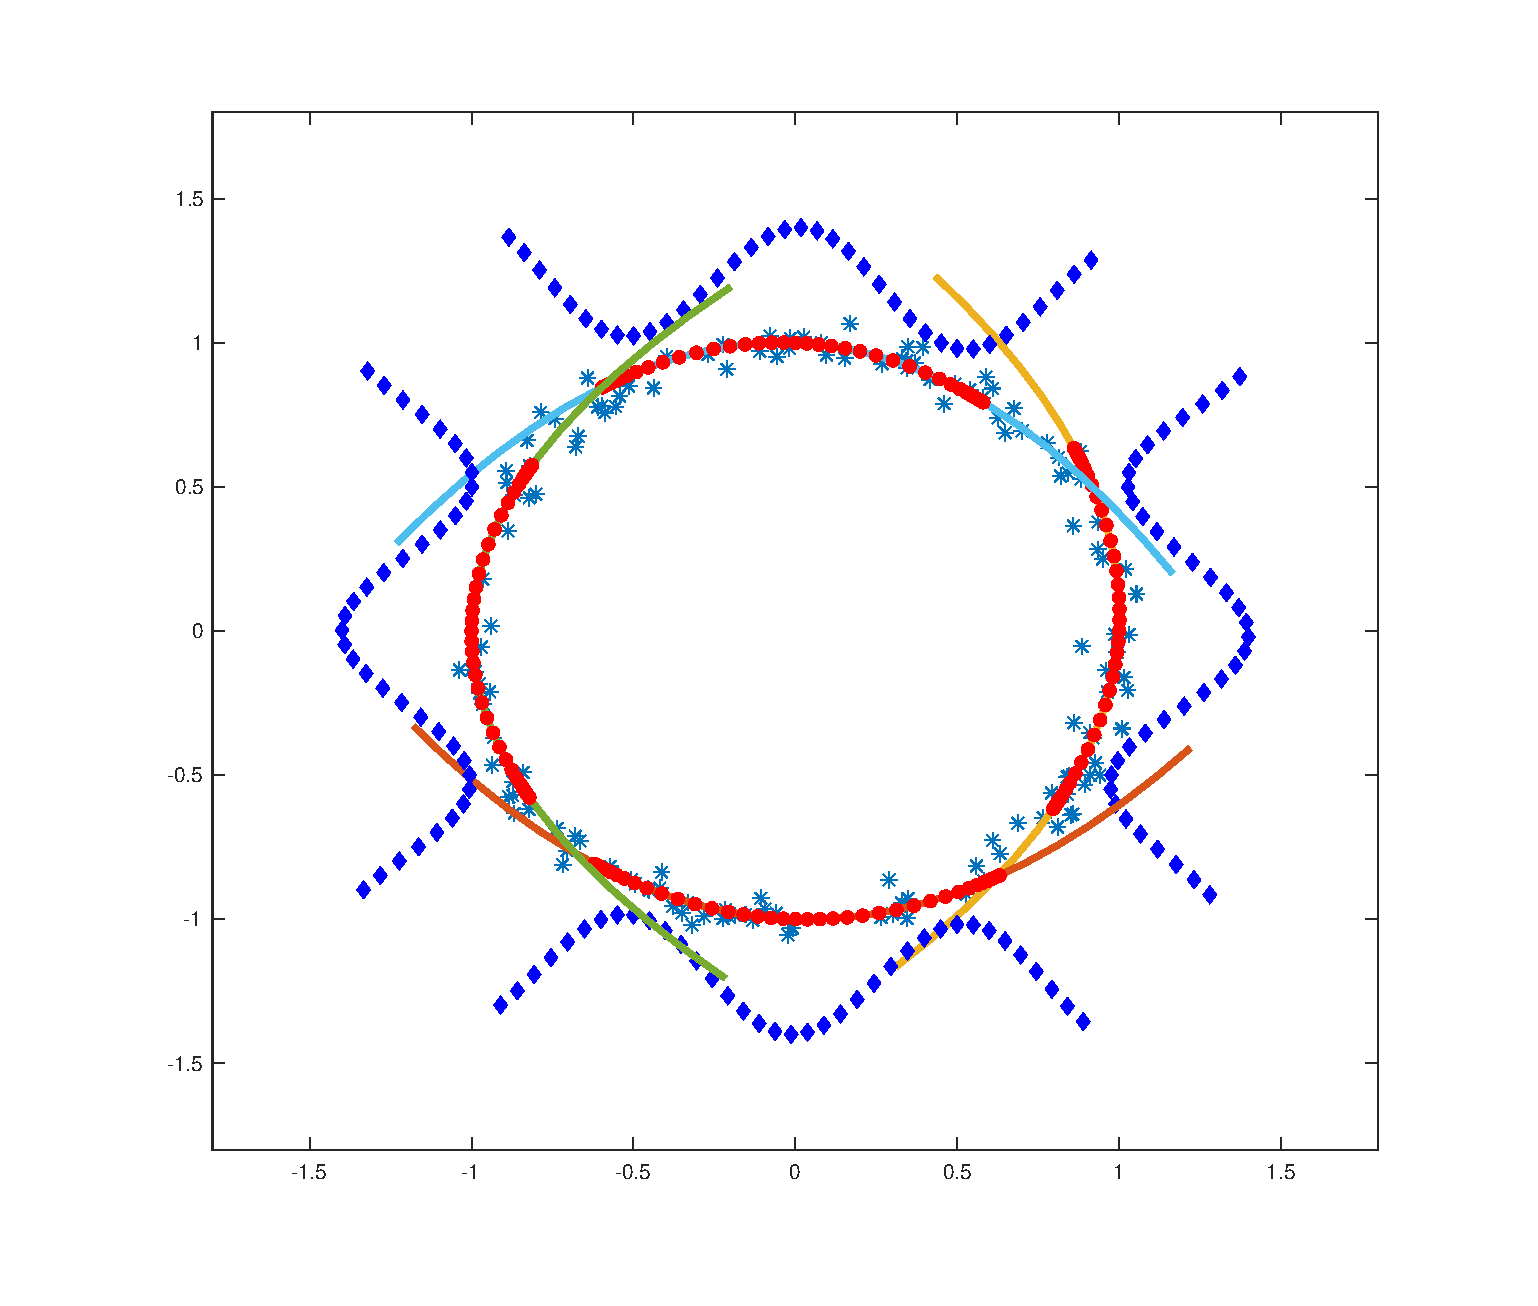
\includegraphics[width=0.65\linewidth]{fit_demo.eps} 
   \caption{Projecting the outlier points onto the fitted manifold}
   \label{fig:example}
\end{figure}

\begin{theorem}
Under the same fitting error tolerance $\epsilon$, the numbers of the fitting structure needed for $x_{\ell}(\tau)$ and $x_{\cal A}(\tau)$ yields
\[
\frac{N(x_{\ell}(\tau), {\cal M}, \epsilon )}{N(x_{\cal A}(\tau), {\cal M}, \epsilon )}=O(\epsilon^{-d/6})
\]
\end{theorem}
\begin{proof}
Define 
$
{\cal M}(x_0,\delta) = \{x| x \in {\cal M},d(x, x_0) \leq \delta\}.
%???\{x| x \in {\cal M},d(x, {\cal \hat{M}}(x(\tau), x_0)) \leq \delta\}
$, For $x\in {\cal M}\cap {\cal D}_{x_0}(\delta)$, we know:
\[
d(x, {\cal \hat{M}}(x_{\cal A}(\tau),x_0)) = O(\|\tau\|_2^3)
\]
Similarly, for the linear fitting function $x_\ell(\tau) = U_d\tau+x_0$ of $\cal M$, we have the projection error is:
\[
d(x, {\cal \hat{M}}(x_\ell(\tau),x_0)) = O(\|\tau\|_2^2)
\]
where $\tau=U_d^T(x-x_0)$ which is the local coordinate of $x$. If we set the maximum tolerance to be 
\[
d(x, {\cal \hat{M}}(x_{\cal A}(\tau),x_0))\leq \epsilon,\quad d(x, {\cal \hat{M}}(x_\ell(\tau),x_0)) \leq \epsilon,
\]
the maximum radius is of order $\epsilon^{1/3}$ and $\epsilon^{1/2}$ for $x_{\cal A}(\tau)$ and $x_{\ell }(\tau)$  respectively.
The corresponding volume of 
\[
\begin{aligned}
&{\rm Vol} \{x| x\in {\cal M},d(x, \hat{\cal M}(x_{\cal \ell}(\tau),x_0))\leq \epsilon \} =O( \epsilon^{d/2})\\
&{\rm Vol} \{x| x\in{\cal M}, d(x, {\cal \hat{M}}(x_{\cal A}(\tau),x_0))\leq \epsilon \} =O(\epsilon^{d/3})
\end{aligned}
\]
As a result, the number of the fitting structure needed is $O( \epsilon^{-d/2})$ and $O(\epsilon^{-d/3})$ for $x_{\cal \ell}(\tau)$ and $x_{\cal A}(\tau)$ respectively. 
\end{proof}

\begin{theorem}
For any $x$, denote the projection of $x$ onto ${\cal M_A}$ as $x^*$ and correspondingly there is the local corrdinate $\tau^*$ such that $x(\tau^*)=x^* $, then we have
\[
x-x^* \perp {\cal T}_{\cal M_A} (\tau^*)
\]
\end{theorem}
\begin{proof}
Recall $x_{\cal A}(\tau) = U_\perp {\cal A}(\tau,\tau)+U(\tau)+x_0$, then the tangent space ${\cal S}^*$ at $x_{\cal A}(\tau)|_{\tau^*}$ is
\[
{\cal S}^* = {\rm span}\{\nabla_{\tau_1} x_{\cal A}(\tau)|_{\tau=\tau^*}, \nabla_{\tau_2} x_{\cal A}(\tau)|_{\tau=\tau^*},...,\nabla_{\tau_d} x_{\cal A}(\tau)|_{\tau=\tau^*}\},
\]
which corresponding to each columns of the Jacobi matrix $J(x_{\cal A}(\tau))|_{\tau^*}$. Note that, the Jacobi $J(x_{\cal A}(\tau))|_{\tau^*}$ is
\[
J(x_{\cal A}(\tau))|_{\tau=\tau^*} = 2U_\perp {\cal A}(\tau^*) + U.
\]
$\cal S^*$ is also the space spanned by the columns of $J(x_{\cal A}(\tau))|_{\tau=\tau^*}$. To prove $x-x^* \perp {\cal T}_{\cal M_A}({x^*})$, we just need to prove $x-x^*$ is orthogonal with each of the columns of $J(x_{\cal A}(\tau))|_{\tau=\tau^*}$. Next, we give the form of $x-x^*$, recall that
\[
\begin{aligned}
x-x^* =& x -  (U_\perp {\cal A}(\tau^*,\tau^*)+U\tau^*+x_0)\\
	=& U_\perp (U_\perp^T(x-x_0) - {\cal A}(\tau^*,\tau^*)) +U(U^T(x-x_0)-\tau^*)\\
	=& U_\perp(c_x - {\cal A}(\tau^*,\tau^*))+U(s_x-\tau^*).
\end{aligned}
\]
It is easy to verify
\[
(x-x^*)^T J(x(\tau))|_{\tau=\tau^*} = -\{({\cal A}(\tau^*){\cal A}(\tau^*,\tau^*)-{\cal A}(\tau^*)c_x) +(\tau^*-s_x)\} = 0,
\]
where the last equality is obtained from the optimal condition in \eqref{normal}, that is to say, $x-x^*$ is orthogonal with the space $\cal S^*$.
\end{proof}

\subsection{Origin Point Selection} \label{Origin Point Selection}
The selection of the origin point $x_0$ is important for our fitting. If our observations $\{x_i\}$ is sampled exactly from $\cal M$ (no noise contaminated), we can select $x_0$ to be the point which is nearest to $\bar{x}$.
\[
x_0 = \arg\min_{\{x_i\}} \|\bar{x}-x_i\|_2
\]
Otherwise, if the observations $\{x_i\}$ are drawn from $\cal M$ with noise, we can select $x_0$ as the weighted-mean as:
\begin{equation}\label{weighted_mean}
x_0 =\frac{1}{\sum_{i\in {\cal N}_k(\bar{x}) } \phi_h(\bar{x},x_i)} \sum_{i\in {\cal N}_k (\bar{x})} \phi_h(\bar{x},x_i)x_i
\end{equation}
where $\phi_h(\bar{x},x_i) = K_h(x_i, \bar{x})$ and ${\cal N}_k$ controls the neighbor size and $h$ is the bandwidth parameter, which affect the bias and smoothness. If we further denote 
\[
w_h(\bar{x},x_i)=\phi_h( \bar{x},x_i) / (\sum_{i\in {\cal N}_k (\bar{x})} \phi_h(\bar{x},x_i))
\]
From \eqref{weighted_mean}, we see that $x_0$ is a convex combination of samples $\{x_i\}$ in the neighborhood ${\cal N}_k(\bar{x})$ of $\bar{x}$ as $x_0 = \sum_{i\in {\cal N}_k (\bar{x})} w_h(\bar{x},x_i) x_i$
\begin{assumption}
Assume the observations are drawn from some manifold, which is parameterized by the form of
\[
x(\tau) = U \tau+ U_\perp {\cal A}(\tau, \tau)+x_0^*.
\]
Thus, $x_i = U \tau_i + U_\perp {\cal A}(\tau_i,\tau_i)+x_0^* +\sigma \epsilon_i$, where $\epsilon_i$ is the independent noise vector such that $\epsilon_i \sim {\cal N}(0, I)$ and $\sigma$ is the scale of the disturbed noise.
\end{assumption}
\begin{theorem}
For any $x_0$ defined as a summation of point in \eqref{weighted_mean},  the squared distance from $x_0$ to the manifold $\cal M_A$ is upper-bounded by
\[
\min_{y\in {\cal M_A}} d (x_0, y) =  \|{\cal A}\|_2^2O(h^4)
\]
%\[
%{\rm E} (\min_\tau \|x_0-x(\tau)\|_2^2) \leq {\rm E} (\|x_0-x(\tau_w)\|_2^2) \leq \max_k(\lambda_{k} ({{\cal A}_{\cdot,\cdot,k}})) O({r}^4h^4)+ {\sigma^2}
%\]
\end{theorem}
The proof is left in the appendix \eqref{dis_x0}.

\section{Algorithm: Projection by Repeated Nonlinear Least Square}\label{nonliear projection}
Because the underlying manifold is unknown, in real computational cases,  we cannot find a point $x_0\in \cal M$ which is also next to our interested outlier $\bar{x}$. To solve this problem, we use an iteration method to find $x_0$. When $\bar{x}$ is far away from $\cal M$, the inaccurate of $x_0$ is also acceptable. With the process of $\bar{x}$ approaching $\cal M$, we need the accuracy of  $x_0$ to be improved.

Our algorithm is consisted of steps by repeatedly implementing the fitting and projection procedures.
%The fitting procedure containing the following three steps:

\vspace{-3mm}\hspace{-4mm}\rule[-10pt]{\linewidth}{0.05em}

\vspace{2mm}\hspace{-4mm}{\bf Repeat: from A1 to B3}

\hspace{-4mm}{\it The fitting procedure contains the following four steps:}
\begin{itemize}
\item[A1.] For outlier $\bar{x}$, compute the shift mean $x_0$ from \eqref{weighted_mean} and use $x_0$ as the origin of our local coordinate to implement our fitting and projection process.
\item[A2.] Given $x_0$, neighborhood size $k$ and bandwidth parameters $h$, get the local coordinate $\{\tau_i, \iota_i\}$ for each $x_i$ by applying the eigenvalue decomposition.
\[
{\tau}_i = U_d^T(x_i-x_0).%,\quad \hat{\iota}_i = {{U^T_{n-d}}}(x_i-x_0)
\]
Using $\tau_i$. construct $G$ from $\{\tau_i\}$ as $G = [g_1,...,g_m]^T$, where each $g_i = {\rm vech}(\tau_i\tau_i^T, 1)$.% is the vectorization form.
\item[A3.] Solve the manifold fitting problem, for the $k$-th dimension in the normal space:
\[
  \min_{\theta_k} \sum_{i=1}^m K_h(x_i-\bar{x})\{ g_i^T \theta_k  -  {(u^k_{x_0})}^T (x_i -x_0)/2\}^2
= \|W_h^{1/2}(G \theta_k-\ell_k/2) \|_2^2,
\]
where the $m$ dimensional vector $\ell_k$ equals to $[u_k^T(x_1-x_0), u_k^T(x_1-x_0),...,u_k^T(x_n-x_0)]$.
\item[A4.] Transform vector $\theta_k$ into matrix by putting the elements of $\theta_k$ onto the upper-diagonal: %of $M_k = {\rm Mat}(\theta_k)$:
\[
S_k = {\rm Mat}(\theta_k) + {\rm Mat}(\theta_k) ^T,
\]
By aligning each slice of $S_k$, we obtain the tensor $\cal A$, i.e., ${\cal A}_{\cdot \cdot k}=S_k$.
Here, we get a simple manifold ${\cal M_A}$ to fit the complicated $\cal M$, where our simple ${\cal M_A}$ yields a form as
\[
x(\tau) = U_{d}^{\perp} {\cal A} (\tau, \tau) + U_d \tau +x_0
\]
\end{itemize}

\hspace{-4mm}{\it The projection procedure contains the following three steps:}
\begin{itemize}
\vspace{2mm}\item[B1.] For an outlier $\bar{x}$, set $\tau_0 = U_d^T(\bar{x}-x_0)$ and apply the fix point iteration, to get the convergence point $\tau^*$ of the sequence $\{\tau_n\}$. The fix point iteration is: 
\[
 \phi(\tau_{n})=( 2{\cal A}(\tau_{n}){\cal A}(\tau_{n})^T+ I_d)^{-1} (2{\cal A}(\tau_{n})c+ s).
\]
\item[B2.] Put $\tau^*$ onto the fitted function  to obtain the point $\hat{x}$, which is the projection of $\bar{x}$ onto ${\cal M}_{\cal A}$ as
\[
\hat{x} = P_{\cal M_A} (x) =  U_{\perp} {\cal A} (\tau^*,\tau^*) + U \tau^* +x_0
\]
\item[B3.] Check whether $\|\hat{x}-\bar{x}\|\leq \epsilon$, if true, stop and output $\hat{x}$, otherwise set $\bar{x}=\hat{x}$ and repeat the steps from A1 to B3.
\end{itemize}
%\hspace{-4mm}\rule[-10pt]{\linewidth}{0.05em}
%\end{table}
\section{Higher-degree extension}
In this section, we give a third-order generalization our manifold fitting algorithm and even higher order generalization approach is similar with the generalization from order-two to order-three.

We split the extension into two parts, fitting a higher order $\cal M_A$, and the projection by solving the nonlinear least square problem details. We show that the higher-degree fitting corresponds to solve a linear least square with more variables than before. 
\subsection{Higher-order manifold fitting}
Recall that for any manifold $\cal M$, there is a corresponding $\phi(\tau)$ such that
\[
x(\tau) = x_0+U \tau+U_\perp \phi(\tau,\tau).
\]
In the above discussion, we approximate $\phi(\tau,\tau)$ by a quadratic form ${\cal A}(\tau_i,\tau_i)$. Besides the quadratic term we also can approximate $\phi(\tau,\tau)$ with the higher order such as
\[
\phi(\tau,\tau) \approx {\cal A}_2 (\tau_i,\tau_i) + {\cal A}_3 (\tau_i,\tau_i,\tau_i),
\]
where ${\cal A}_2$ and ${\cal A}_3$ are the third and forth order tensor of shape $d\times d\times (D-d)$ and $d\times d\times d\times (D-d)$, respectively. Similarly, we can also define $g_i$ by vectorizing $\tau_i\tau_i^T$ and $\tau_i\otimes \tau_i\otimes \tau_i$. Note that, because of the symmetric property of the tensor, for the $k$-th slice of ${\cal A}_2$ and ${\cal A}_3$ there are $d(d+1)/2$ and $d(d^2+1)/2$ free parameters to be determined. In the third order approximation, both of $\theta_k$ and $g_i$ are with the total number of free parameters $(d^3+d^2+2d)/2$.
Similarly, with the samples $\{x_i\}$, we have
\begin{equation*}
  \min_{\theta_k} \sum_{i=1}^m K_h(x_i-x_0)\{ g_i^T \theta_k  - \frac{1}{2} {(u^k_{x_0})}^T (x_i -x_0)\}^2
= \|W_h^{1/2}(G \theta_k-\ell_k) \|_2^2,
\end{equation*}
By realigning the elements in $\theta_k$, we can obtain the $k$-th slice for the tensors ${\cal A}_2$ and ${\cal A}_3$.
\subsection{Projection}
Since $\cal M_A$ is a smooth approximated manifold, the projection onto the fitted manifold $\cal M_A$ is equivalent to solve the minimization problem
\begin{equation}\label{min_higher}
\begin{aligned}
&\min_\tau \|z -  U_{\perp} (({\cal A}_2 (\tau,\tau)+{\cal A}_3 (\tau,\tau,\tau)) + U \tau +x_0)\|_2^2\\
=&\min_\tau \|U^T (z-x_0)-\tau\|_2^2+\|U^T_{\perp}(z-x_0)- {\cal A}_2 (\tau,\tau)-{\cal A}_3 (\tau,\tau,\tau)\|_2^2.
%=& .
\end{aligned}
\end{equation}
Denote $s=U^T (z-x_0), c =U^T_{\perp}(z-x_0)$, the problem \eqref{min_higher} turns to
\[
\min_\tau g(\tau)= \|s-\tau\|_2^2+\|c- {\cal A}_2 (\tau,\tau)-{\cal A}_3 (\tau,\tau,\tau)\|_2^2.
\]
 Define the auxiliary quadratic function $f(\tau_1,\tau_2)$ to approximate $g(\tau)$ as
\[
f(\tau_1,\tau_2) = \frac{1}{2}\|s-\tau_1\|_2^2+ \frac{1}{2}\|s-\tau_2\|_2^2+\|c- {\cal A}_2 (\tau_1,\tau_2)-{\cal A}_3 (\tau_1,\tau_1,\tau_2)\|_2^2.
\]
Then, the alternating minimization iteration will become
\begin{equation}\label{minimi}
\tau_{n+1} = \arg\min_\tau \frac{1}{2}\|s-\tau\|_2^2+\|c- {\cal A}_2 (\tau_n,\tau)-{\cal A}_3 (\tau_n,\tau_n,\tau)\|_2^2.
\end{equation}
Since ${\cal A}_2 (\tau_n,\tau)$ and ${\cal A}_3 (\tau_n,\tau_n,\tau)$ can also be written as the matrix-vector multiplication as
\[
{\cal A}_2 (\tau_n,\tau) = {\cal A}_2 (\tau_n) ^T \tau,\quad {\cal A}_3 (\tau_n,\tau_n,\tau) = {\cal A}_3 (\tau_n,\tau_n)^T \tau.
\]
Note that, both of ${\cal A}_2(\tau_n)$ and ${\cal A}_3(\tau_n,\tau_n)$ are the $d\times (D-d)$ matrix , then, the above minimization problem \eqref{minimi} has the closed-form solution as
\[
 \phi(\tau_{n})=( 2{\cal A}_2(\tau_{n}){\cal A}(\tau_{n})^T+2{\cal A}_3(\tau_{n},\tau_n){\cal A}_3(\tau_{n},\tau_n)^T+ I_d)^{-1} (2({\cal A}_2(\tau_{n})+{\cal A}_3(\tau_{n},\tau_n))c+ s).
\]

Using $\phi(\tau_{n})$, we can also build the fix point iteration as $\tau_{n+1} =  \phi(\tau_{n})$ and obtain the convergence point as the projection onto the third-order manifold fitted function.

From analyzing the two steps of fitting and projection, we can see our model can be easily generalized into a higher-order approximation form. However, because of the number of unknown parameters increases with the speed of $d^s$, where $s$ is the order and $d$ is the dimension of the tangent space, we need large amount of effective data to fix the higher-order model. Otherwise, too small dataset and quit complicate model will lead to the overfitting problem, which will also diminish the performance of our algorithm.
\section{Simulation}
In this section, we compare our nonlinear manifold fitting approach with the existing manifold fitting methods on various occasions. We consider the manifolds having constant curvature and varying curvature. The numerical results show our model can handle all the cases by leading a very promising result.
\subsection{Data Recovery Capability}
In this section, we construct some artificial manifolds e.g triangle cure, circle and the swiss-roll, which can be written as a parameterization form as
$
\left\{
\begin{array}{c}
x = \phi(t)\\
y = \psi(t)
\end{array}
\right.
$
Thus, we have the tangent space is spanned by $(\phi'(t),\psi'(t))$ and the normal space is spanned by the vector $(\psi'(t),-\phi'(t))$. The curvature at $t$ can be calculated as
\begin{equation}\label{kappa}
\kappa(t) = \frac{\phi'(t)\psi''(t)-\phi''(t)\psi'(t)}{((\phi'(t))^2+\psi'(t)^2)^{3/2}}
\end{equation}
Especially, when the curve parameterized as $(x,f(x))$, the curvature yields quite a simple form as
%manifold case of the triangle curve 
%\[
%f(x)=\sin(x).
%\]
%This curve has a variation curvature depending on $x$. Note that, 
$\kappa(x) = \frac{|f''(x)|}{(1+f'(x))^{3/2}}$. Next, we give three examples and show the performance of our algorithm.
\begin{example}
By substituting the derivatives of the 2-D circle's parametric equation  into \eqref{kappa}. we know that the curvature of the circle $\left\{\begin{array}{c}
x= \cos(\theta)\\
y=\sin(\theta)
\end{array}\right.$ is the constant $\kappa(\theta) = 1$ everywhere, 
\end{example}
\begin{example}
For the swiss-roll in the 2-D space, the parametric equation is $\left\{ \begin{array}{c} x=\theta\cos(\theta)\\ y = \theta\sin(\theta)\end{array}\right.$. Thus, we have the first derivatives and the second derivatives:
\begin{equation}\label{derivative_swiss}
\begin{aligned}
&x'(\theta)=\cos(\theta)-\theta\sin(\theta),\quad y'(\theta)=\sin\theta+\theta\cos\theta\\
&x''(\theta)=-2\sin\theta-\theta\cos\theta,\quad y''(\theta)=2\cos(\theta)-\theta\sin(\theta).
\end{aligned}
\end{equation}
Substitute \eqref{derivative_swiss} into the equation of curvature, we have $\kappa(\theta)=\frac{2+\theta^2}{(1+\theta^2)^{3/2}}$ and $\kappa'(\theta) =\frac{ -\theta(\theta^2+4)}{(1+\theta^2)^{5/2}}$. For any $\theta\in {\mathbb R}^+$, the curvature decreases with the increasing of $\theta$.
\end{example}
\begin{example}
Recalling the function of the triangle curve 
$\left\{
\begin{array}{l}
x(\theta)=\theta\\
y(\theta)=\sin \theta
\end{array}
\right.$ and taking the derivatives with respect to $x$, we know that
\[
x'(\theta) = 1,\quad y'(\theta)= \cos(\theta),\quad x''(\theta)=0, \quad y''(\theta) = -\sin(\theta)
\]
By substituting the derivatives into the equation of the curvature, we know $\kappa(\theta)$ of the triangle curve $(\theta, \sin \theta)$ at $\theta$ is
$
\kappa(\theta) =  \frac{|\sin(\theta)|}{(1+\cos(\theta))^{3/2}},
$
which achieves the maximum $\kappa(\theta)=1$ when $\theta=k\pi+\frac{1}{2}\pi, k\in Z$ and $\kappa(\theta)$ achieves the minimum $\kappa(\theta)=0$ when $\theta=k\pi, k\in Z$, which could also be observed from the curve of the function.
\end{example}
\begin{remark}
The first 2-D circle example is a curve with constant curvature and the remaining two examples are curves with varying curvature. The swiss-roll is an example which has the curvature monotonously decreasing with the parameter $\theta$. The triangle curve is an example which has periodic curvature with respect to the parameter.
\end{remark}

\begin{figure}[t] %  figure placement: here, top, bottom, or page
   \centering
    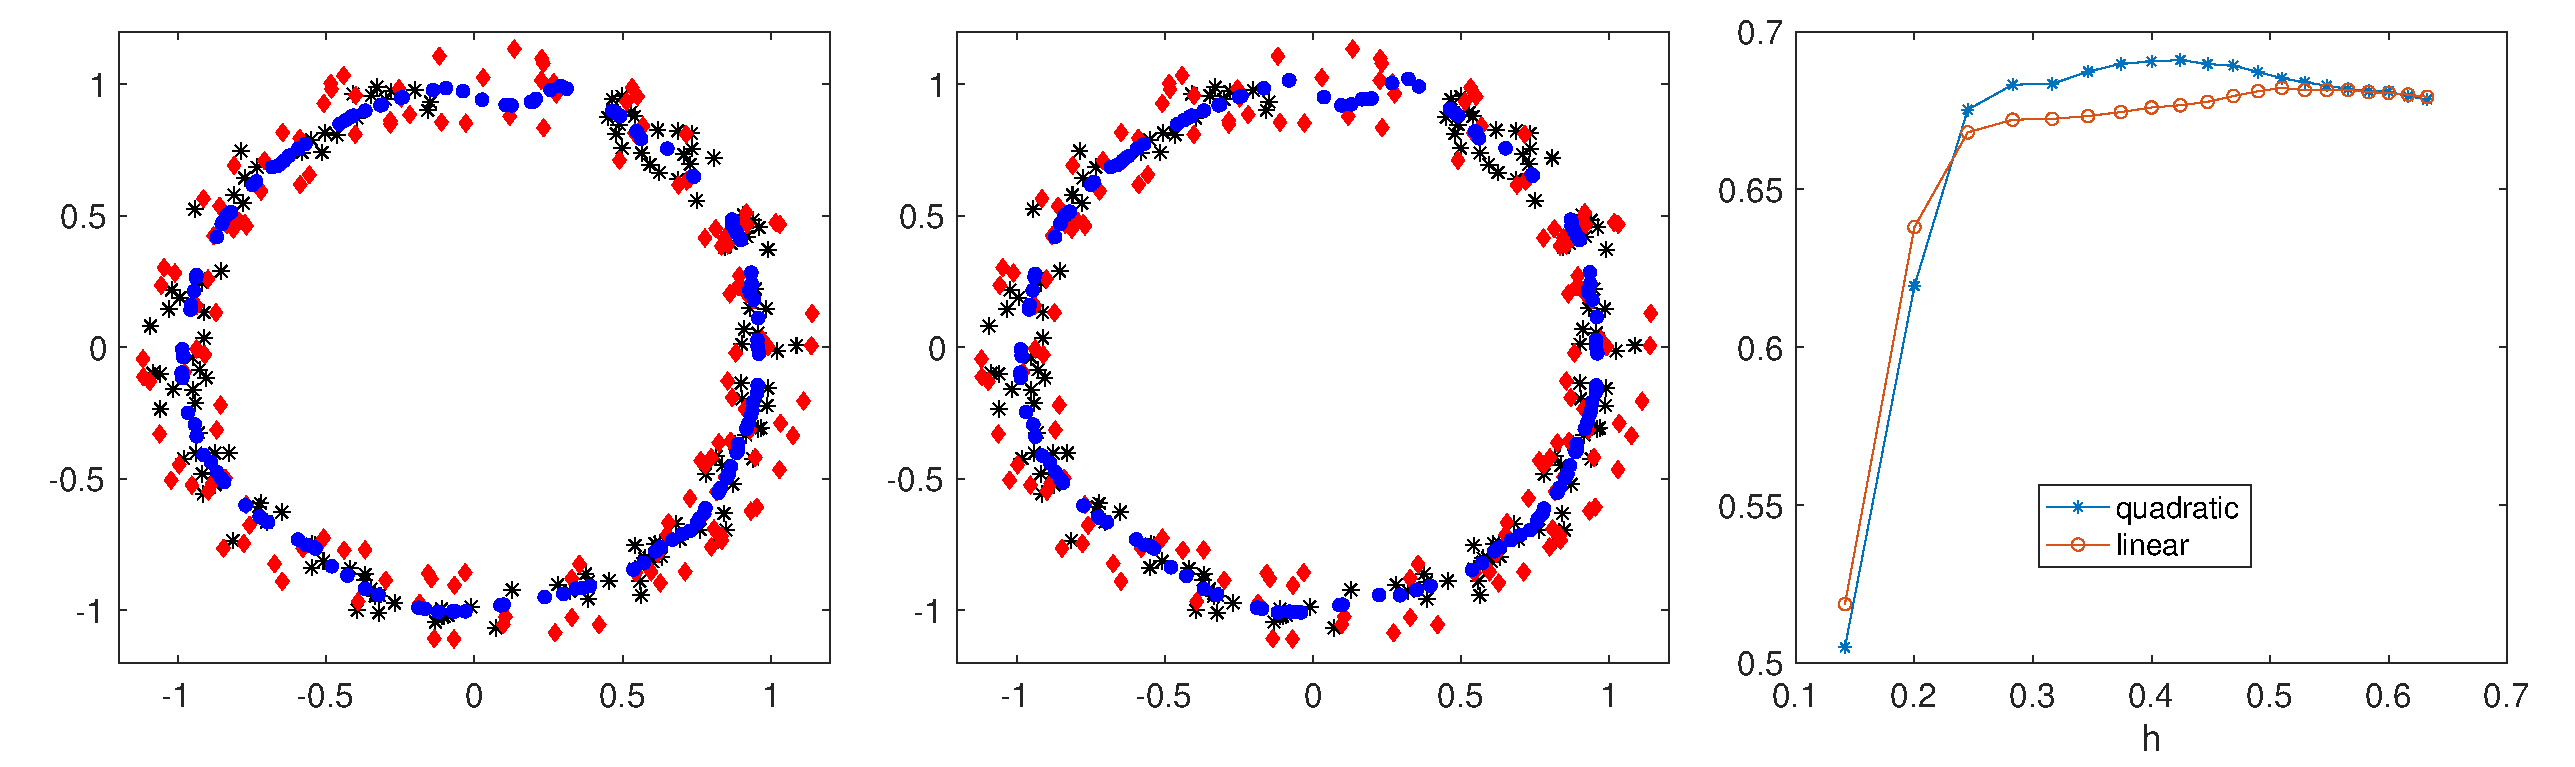
\includegraphics[width=\linewidth]{circle_result.eps} 
     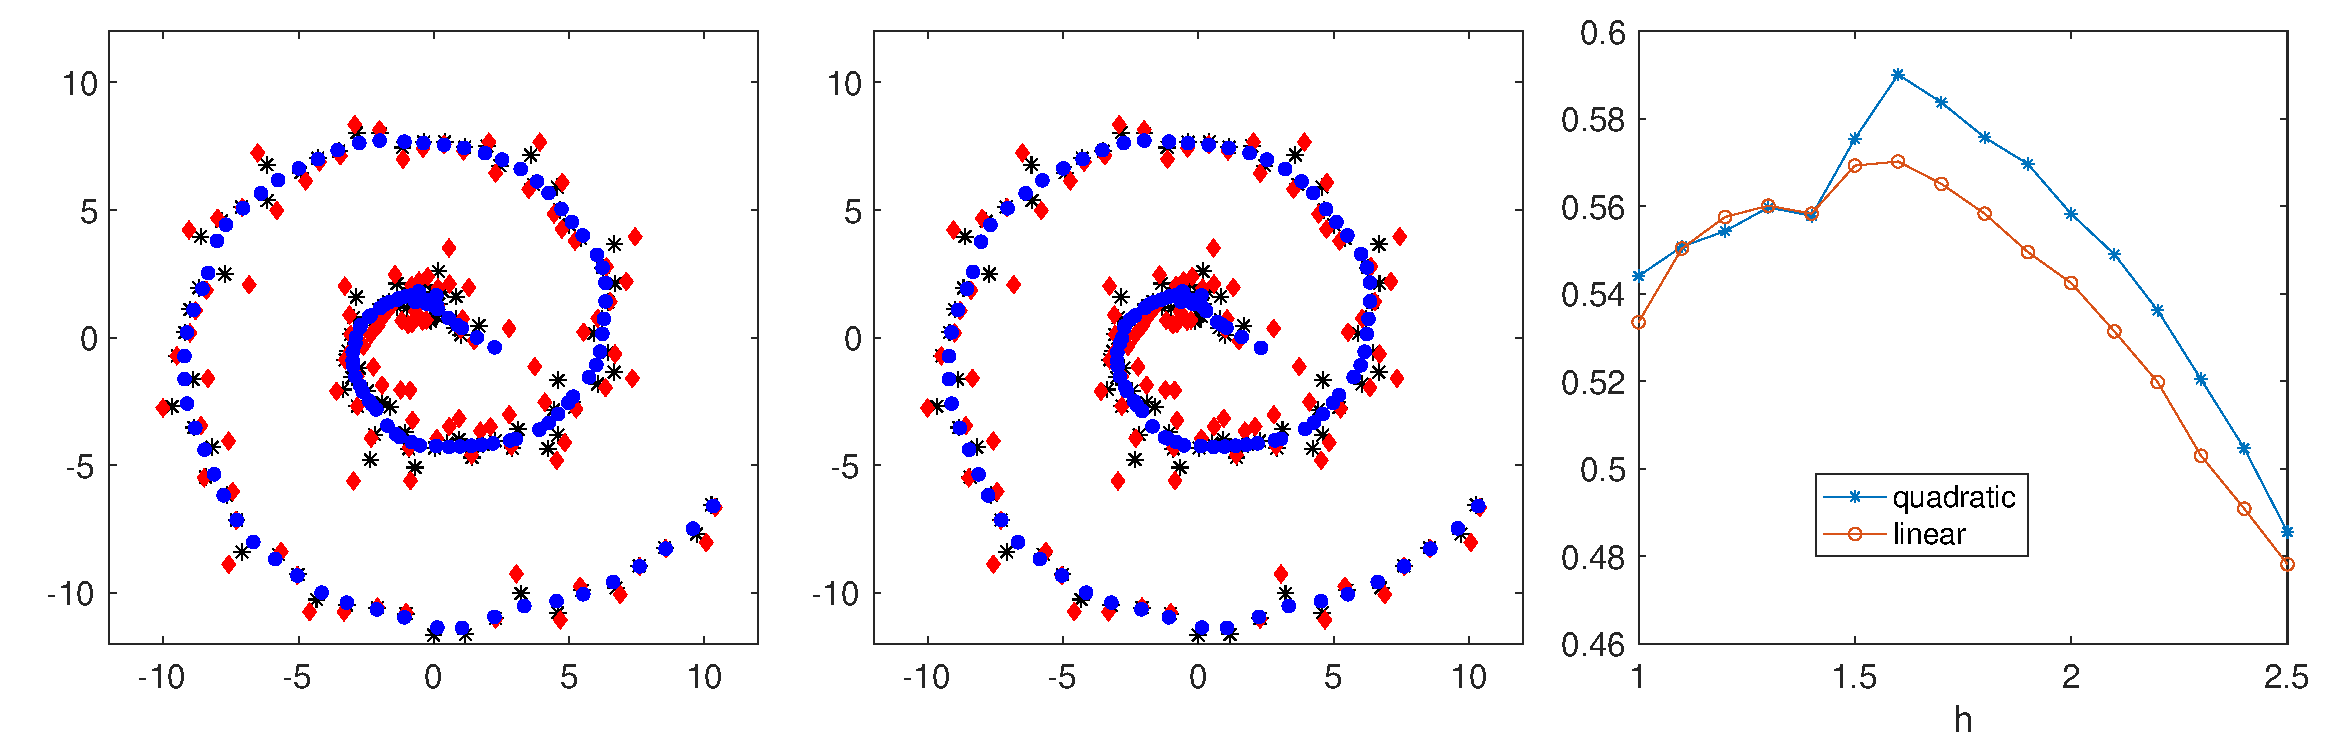
\includegraphics[width=\linewidth]{swiss_roll.eps} 
     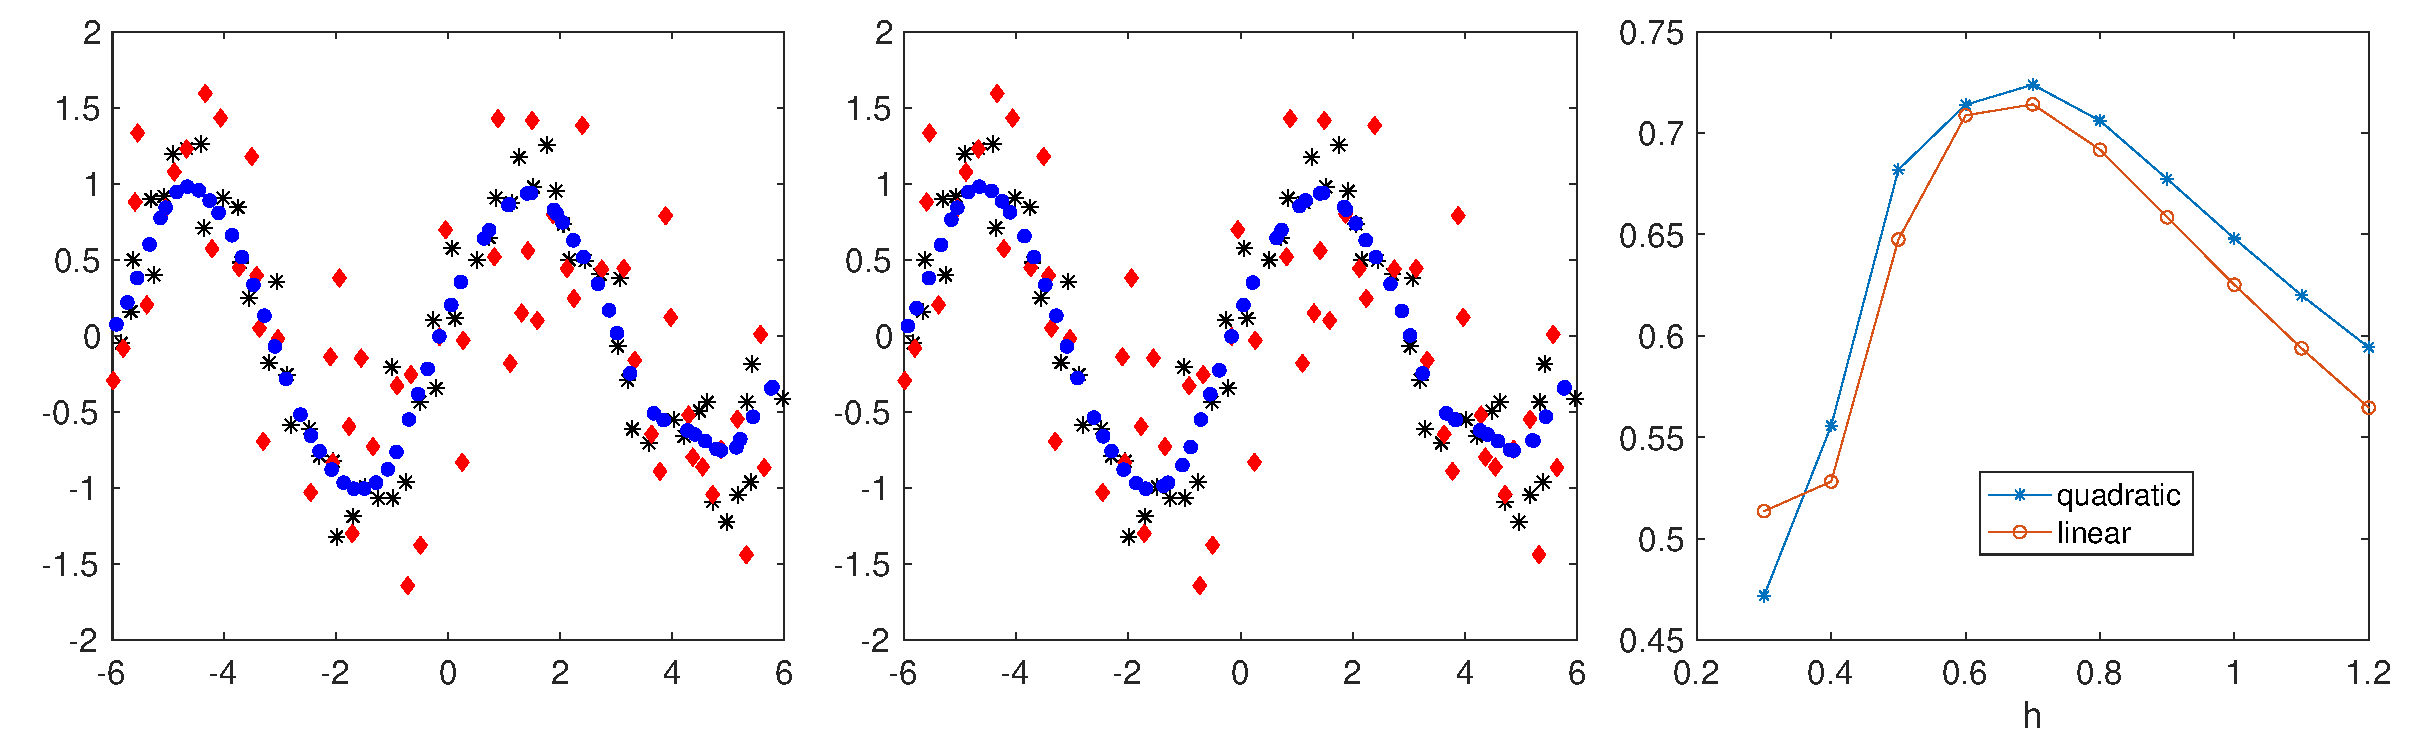
\includegraphics[width=\linewidth]{sin_curve2.eps} 
   \caption{Comparison between nonlinear projection and linear projection. Left: nonlinear approach. Right: linear approach}
   \label{fig:sin_curve}
\end{figure}

It is difficult to fit the data drawn from a manifold which is assumed to have varying curvature using a linear model or a tangent plane. Because for $x$ in an area which leads $\kappa(\theta)$ small, the manifold can be approximated by a low-dimensional affine space (a flat plane). However, in a area which has the large curvature $\kappa(\theta)$, such as $\theta=\pi/2$ in our triangle curve case, it is impossible to approximate $y = \sin(\theta)$ by a flat structure. Therefore, it is quit necessary to use a more complicated model to approximate. 

Noting that, our nonlinear second-order fitting function $x_{\cal A}$ is a generalization of the linear function $x_\ell$. When the second order parameter $\cal A$ equal to zero, the derived manifold $\cal M_A$ will degenerate into ${\cal M}_\ell$. By learning $\cal A$, we automatically considering the curvature information hidden in the manifold.


Since our nonlinear second-order fitting model $\cal M_A$ is more complicated by having more parameters compared with ${\cal M}_\ell$, we need to use more data to solve our model. Solving the least square problem with too few data will lead to a phenomenon called `overfitting'. When the overfitting phenomenon occurs, the model will not only learn from the true signal of the underlining manifold, but also the noise factors which will distort our model.

In our fitting model, the number of points used is controlled by the bandwidth parameter $h$. Because the kernel weight is decreased fast with the radius, the contribution of the points resides far from our interested area is ignorable. As a result, our model works well with a relatively larger $h$, which can be seen in the rightmost partition of Figure \eqref{fig:sin_curve}.



In Figure \eqref{fig:sin_curve}, we randomly samples the black stars `*' as $x_i = \tilde{x}_i+\sigma_1\epsilon_i$ and the red diamonds `$\diamond$' as $x_i = \tilde{x}_i+\sigma_2\epsilon_i$, where $\tilde{x}_i$ is on the underlining $\cal M$ and $\epsilon_i$ is in the normal space of $\cal M$ at $\tilde{x}_i$. In our experimental setting, we have $\sigma_1=0.2$ and $\sigma_2=0.5$ and the length of $\epsilon_i$ obeys the normal distribution of $N(0,1)$. The blue dots `$\circ$' represent the result, which is the projection onto the fitted structure. The leftmost figure is the result obtained from the projection onto the nonlinear $\cal M_A$ and the middle figure stands for the result obtained from the projection onto $\cal M_\ell$.

To evaluate the performance of different results, we define the criteria $c({\hat{\cal M}})$ which represents the percentage of improvement of the corresponding algorithm
\[
c({\hat{\cal M}}) = 1-\frac{d(\hat{\cal M}, {\cal M})}{d({\cal D}, {\cal M})},
\] 
where $\cal D$ stands for the set corresponding to `$\diamond$' which is the outlier we want to pull towards the underlining $\cal M$ and $\hat{\cal M}$ stands for the set corresponding to `$\circ$' which is the result of different methods. The distance of $d({\cal D}, {\cal M})$ is defined as:
\[
d({\cal D}, {\cal M}) = \frac{1}{n} \sum_{x_i\in {\cal D}} \|x_i-\tilde{x}_i\|_2 = \frac{1}{n} \sum_{x_i\in \cal D} \sigma_2\|\epsilon_i\|_2,
\] 
and by replacing $\cal D$ with $\hat{\cal M}$, we could similarly get $d(\hat{\cal M}, {\cal M})$.

The rightmost figure shows that with the increasing of the bandwidth $h$, the nonlinear projection result has a better performance (under the measurement of $c({\hat{\cal M}})$) in data recovery aspect compared with the linear projection.

%\begin{figure}[t] %  figure placement: here, top, bottom, or page
%   \centering
%   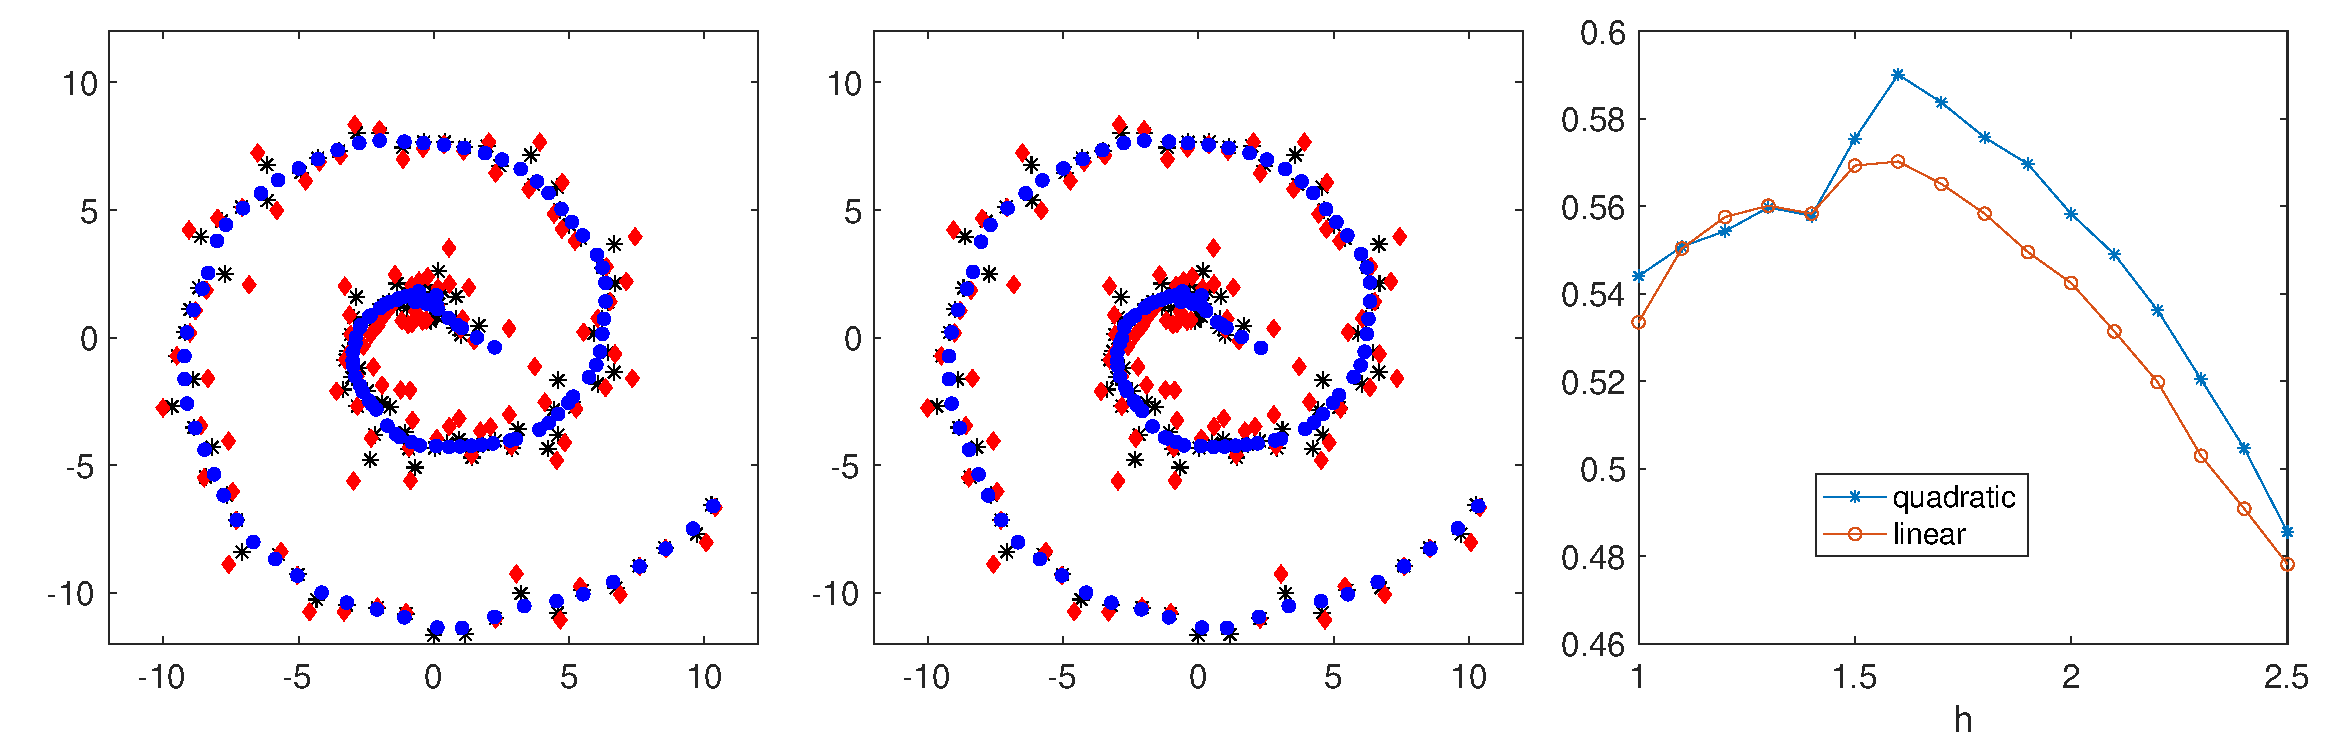
\includegraphics[width=\linewidth]{swiss_roll.eps} 
%   \caption{Comparison between nonlinear projection and linear projection. Left: nonlinear approach. Right: linear approach}
%   \label{fig:sin_curve}
%\end{figure}
\subsection{Orthogonal Property}
In this section, we give a simple case to show the effectiveness of nonlinear projection compared with the linear projection.
\begin{figure}[h] %  figure placement: here, top, bottom, or page
   \centering
   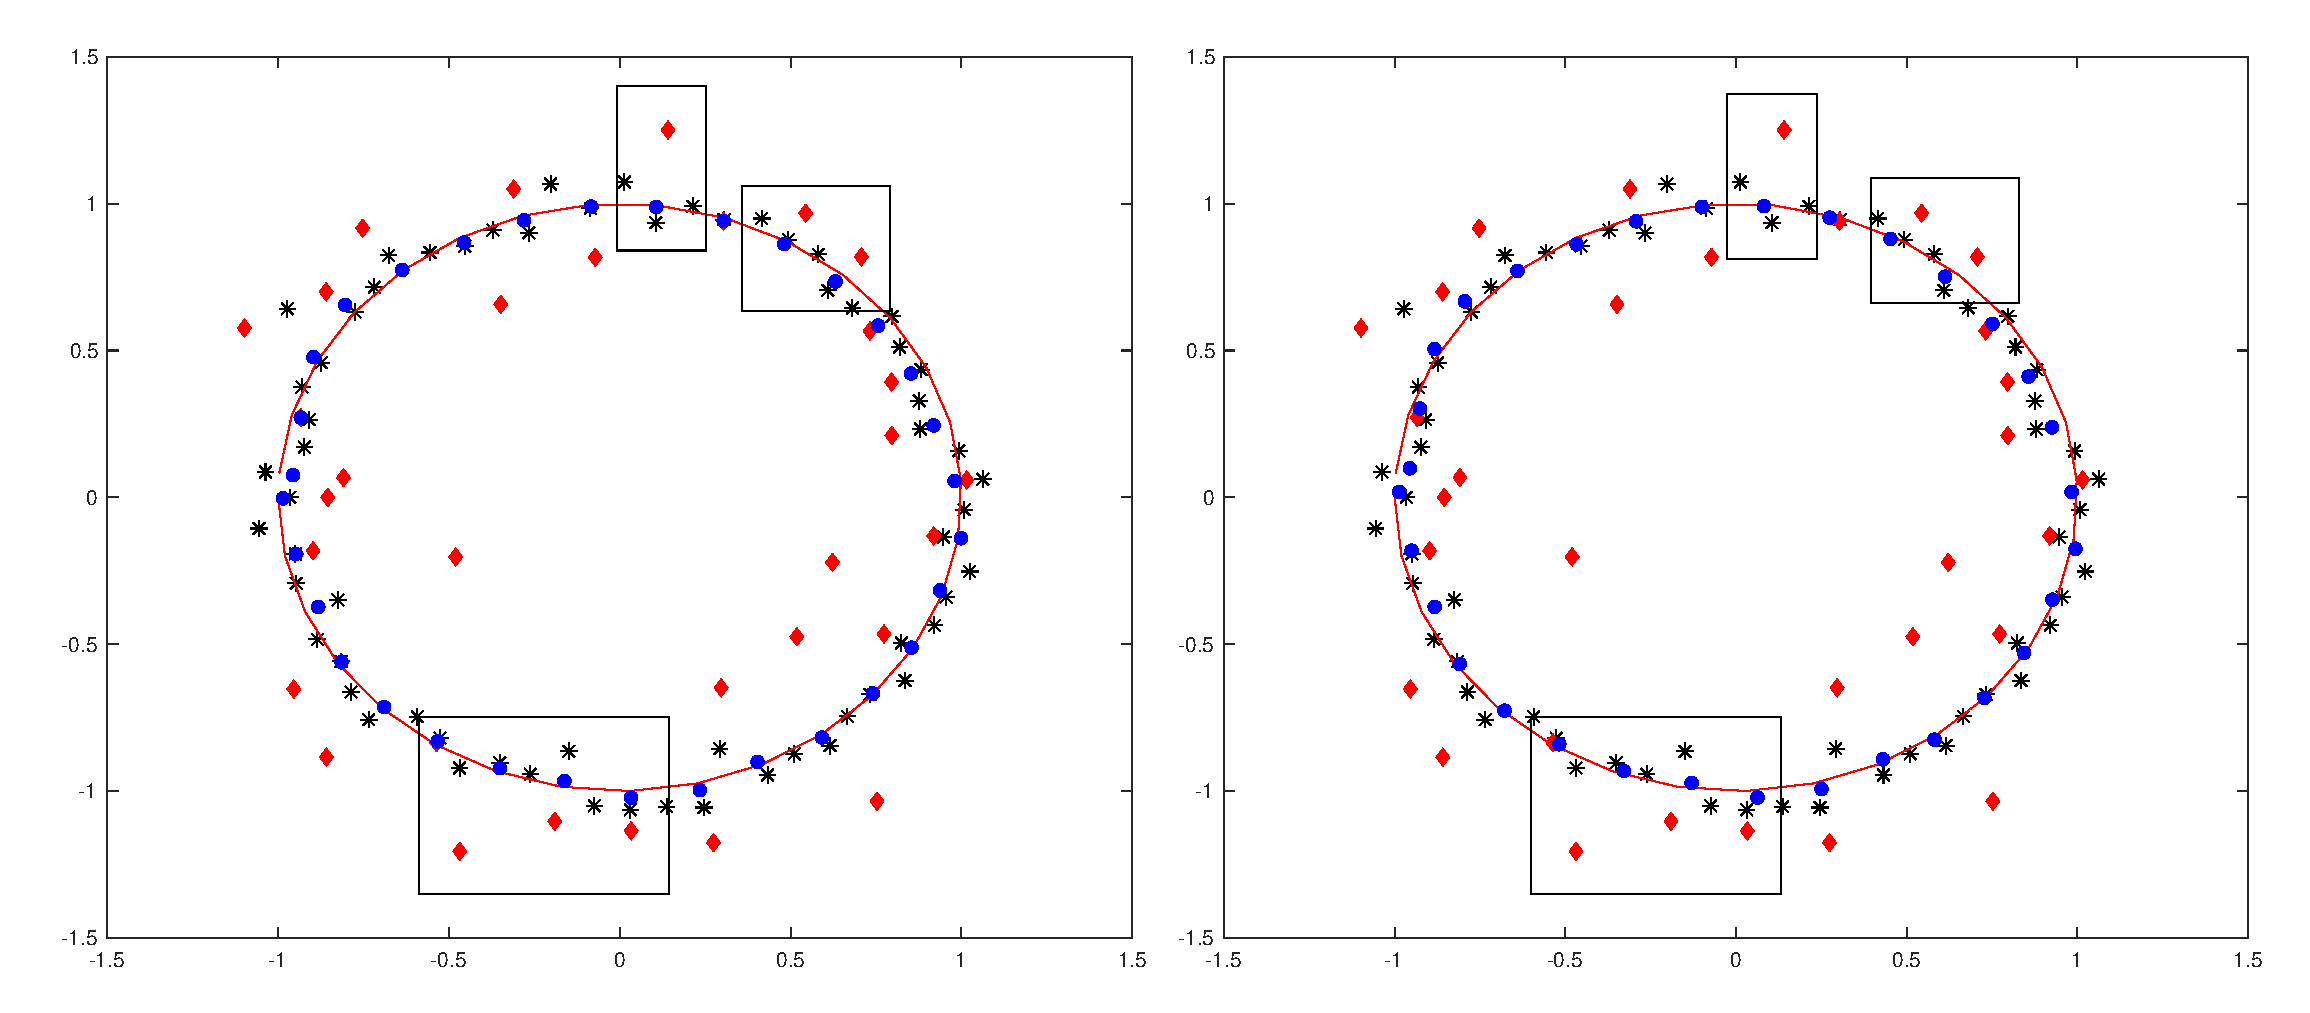
\includegraphics[width=0.7\linewidth]{compare_linear_nonliear.eps} 
   \caption{Comparison between nonlinear projection and linear projection. Left: nonlinear approach. Right: linear approach}
   \label{fig:example}
\end{figure}

Here, we give a brief explanation about the graph. The black stars $*$ represent the observations which is supposed to sampled from some manifold $\cal M$. The red diamonds $\diamond$ represent the outlier points which we want to project onto $\cal M$. Because $\cal M$ is unknown, we need to fit it locally with two different approaches. The red curve represents the true manifold. The red circles $\circ$ represent the projection of the diamonds $\diamond$ projected on the fitted locally defined manifold.

The procedure of projection can be seen in section \ref{nonliear projection}, which can be described in a few steps.
\begin{itemize}
\item[A. {\it Locate the origin}]: For each outlier point $x$, determine the origin $x_0$ corresponding to $x$, such as in \eqref{weighted_mean}.
\item[B. {\it Fit the manifold}]: Corresponding to $x$, fit  with the observations to obtain the local defined function $\tilde{x}(\tau)$ and $x_\ell(\tau)$, i.e, get the respective parameters $\cal A$, $U_d$, $U_d^\perp$.
\item[C. {\it Project backwards}]: Project $x$ onto the fitted manifold ${\cal M}_s$ defined by the function $\tilde{x}(\tau)$ by the repeatedly nonlinear least square. Project $x$ onto the manifold ${\cal M}_\ell$ defined by the function $x_\ell(\tau)$ using the linear projection.
\end{itemize}
For fairness of the comparison, we use the same central point $x_0$ as \eqref{weighted_mean}. The difference between this two methods owns to the different function which locally approximate the manifold. The two functions can be summarised as the function of the linear affine space and the function of high-dimensional surface:
\[
{x}_{\cal A}(\tau) = U_{d}^{\perp} {\cal A} (\tau, \tau) + U_d \tau +x_0, \quad x_\ell(\tau) =  U_d \tau +x_0
\]
The criteria for a better projection is to require the projection implement exactly in the normal space. %To evaluate the performance, we want the projection vector $x-P_{{\cal M}_s}(x)$ and $x-P_{{\cal M}_\ell}(x)$
We want the vector $x-P_{{\cal M}}(x)$ to be perpendicular with the tangent space of $\cal M$ at the projected point $P_{{\cal M}}(x)$, i.e., 
\[
x-P_{{\cal M}}(x)\perp {\cal T}_{\cal M} (P_{{\cal M}}(x))
\]
From the above two figures, we can see the left figures is with high quality, that is, almost all points projected onto $\cal M$ within the normal space, especially for the points emphasized in the rectangle.
\subsection{Parameters Reliance}
There are two parameters (the bandwidth $h$ and neighborhood size $k$), which affect the performance of our algorithm. In this section, we show the relationship between the fitting property and the parameters.  We use the color to represent the average approximation error ${\rm Error}({\cal M}_{\cal A},{\cal M},\{x_i\})$, which is defined by
\[
{\rm Error}({\cal M}_{\cal A},{\cal M},\{x_i\}) = \frac{1}{n}\sum_i \|P_{{\cal M}_{\cal A}}(x_i) -P_{{\cal M}} (x_i)\|_2
\]
where $P_{{\cal M}} (x_i)$ is the projection of $x_i$ onto $\cal M$ and $P_{{\cal M}_{\cal A}}(x_i) $ is the projection of $x_i$ onto the fitted manifold ${\cal M}_{\cal A}$.
\begin{figure}[h] %  figure placement: here, top, bottom, or page
   \centering
   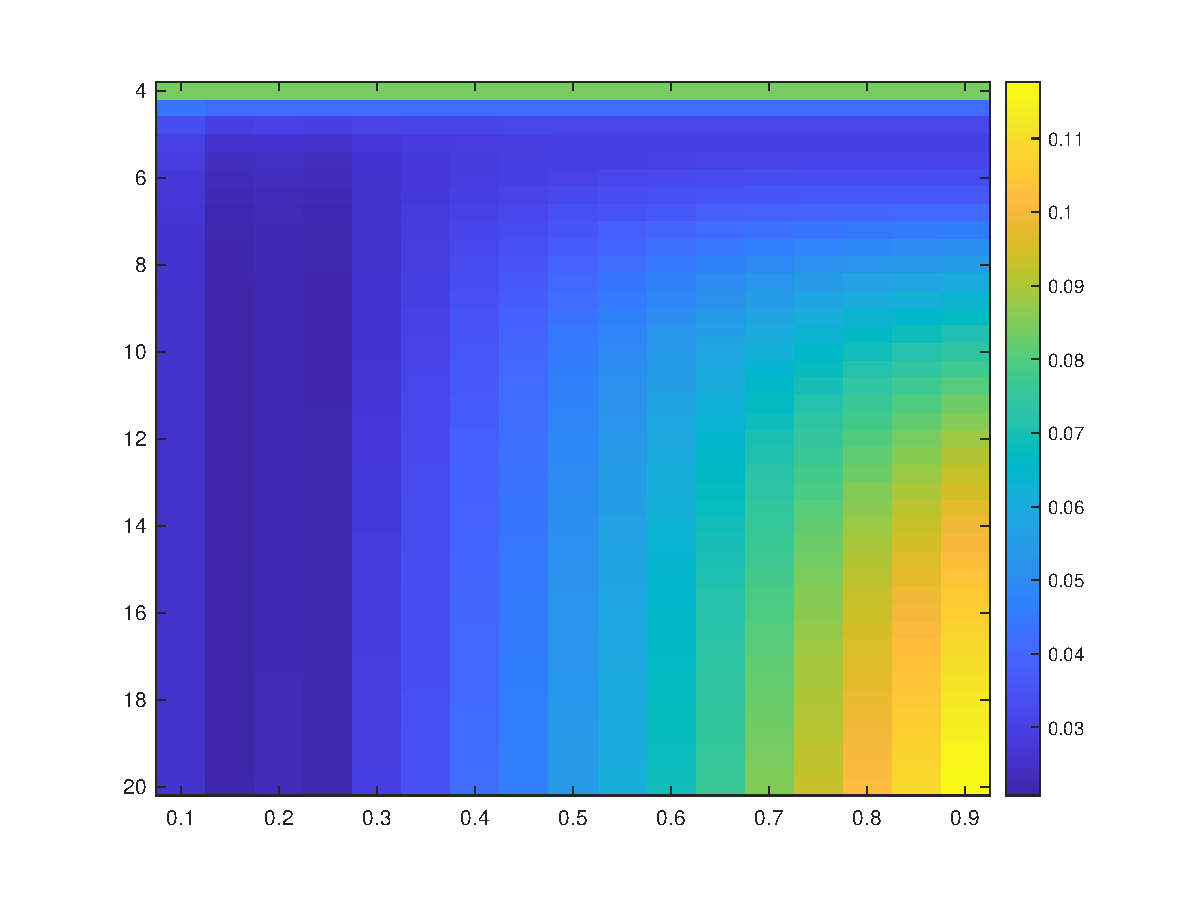
\includegraphics[width=0.6\linewidth]{parameter_rh.eps} 
   \caption{Parameters reliance of ${\rm Error({\cal M}_{\cal A})}$ on the bandwidth $h$ (horizontal axis) and the neighborhood size $k$(vertical axis).}
   \label{results on parameters}
\end{figure}

In Figure \eqref{results on parameters}, the dark blue color represents a good fitting standard with the corresponding parameters. We can see that setting smaller bandwidth $h$ or restricting within a smaller neighborhood $k$ has a similar effect on ${\rm Error({\cal M}_{\cal A})}$. However, $h$ also cannot be too small. When $h\rightarrow 0$, because of initial point and the estimated tangent turning bad with the increasing of the variance in the observations, the fitting criteria will become large indicating the fitted function gradually turns bad.

\begin{appendix}
\section{}
\subsection{Asymptotic Property}
\begin{proof}
Recall from \eqref{solution} that the estimated $\hat{\theta}_k$ has a closed-form:
\begin{equation}\label{theta_hat}
\hat{\theta}_k = (G^TW_hG)^{-1} G^T W_h\ell_k.
\end{equation}
Note that, $\ell_k$ is the vector and the $i$-th elements represents  the function value of $\phi_k(\tau_i)/2$. Because the Taylor expansion of $\phi_k(\tau)$ at $\tau=0$ satisfied
\[
\phi_k(0) = 0, \quad \nabla_\tau \phi_k(\tau)|_{\tau=0} = 0.
\]
%which consists of $(\ell_k)_i = \frac{1}{2}\phi_k(\tau_i)$, is
Thus, we have the Taylor expansion starting from the term of order 2 as
\begin{equation}\label{Taylor_phi}
\frac{1}{2}\phi_k(\tau_i) = g_i^T\theta_k+t_i^T \eta_k+O(\|\tau_i\|_2^4),
\end{equation}
where $\theta_k = {\rm vech}(\nabla\nabla\phi_k(\tau)|_{\tau=0}), \eta_k={\rm vech}(\nabla\nabla\nabla\phi_k(\tau)|_{\tau=0})$, which is a vectorization of the third order derivative of $\phi_k(\tau)$ and $t_i^T$ is the vectorization of the tensor $\tau_i\otimes \tau_i\otimes \tau_i$. Rewritting \eqref{Taylor_phi} in vector form, we have
\begin{equation}\label{ell_k}
\ell_k = G\theta_k+T\eta_k+O(\|\tau_i\|_2^4),
\end{equation}
where $T$ is a matrix and each row of $T$ is $t_i^T$. Substitute \eqref{ell_k} into \eqref{theta_hat}, we have
\[
\begin{aligned}
\hat{\theta}_k - \theta_k &= (G^TW_hG)^{-1} G^T W_h\ell_k - \theta_k\\
&= (G^TW_hG)^{-1} G^T W_h(T\eta_k+O(\|\tau_i\|_2^4))
\end{aligned}
\]
Next, we give an estimation with the order of $G^TW_hG$ and $G^T W_hT$. Firstly, the expectation
\[
\begin{aligned}
&{\rm E} (\frac{1}{n}G^TW_hG) \\
%= &\int {\rm vech}(\tau\tau^T)  {\rm vech}^T(\tau\tau^T) K_h(y-x)d\tau\\
= &\frac{1}{h^D}\int_{y\in {\cal M}} {\rm vech}(U^T(y-x) (y-x)^T U)  {\rm vech}(U^T(y-x) (y-x)^T U) K_h(y-x)p(y)d y.
\end{aligned}
\]
Letting $z = {(y-x)}/{h}$, we have ${1}/{h^D}dy = dz$. Changing the integrating variable from $y$ to $z$, we have the expectation ${\rm E} (G^TW_hG/n)$ and ${\rm E} (G^TW_hT/n)$ becoming
\begin{equation}\label{expectation1}
\begin{aligned}
&{\rm E} (G^TW_hG/n) \\
= & h^{4} p(x) \int {\rm vech}(U^T zz^TU)  {\rm vech}^T(U^T zz^TU) K(z) p(x+hz)d z\\
= &h^{4} p(x) \int {\rm vech}(U^T zz^TU)  {\rm vech}^T(U^T zz^TU) K(z)d z + O(h^5)
\end{aligned}
\end{equation}
Similarly as the expectation derivation procedure in \eqref{expectation1}  for ${\rm E} (G^TW_hG/n)$, we have the expectation
\begin{equation}\label{expectation2}
\begin{aligned}
&{\rm E} (G^TW_hT/n) \\
= &h^{5} \int {\rm vech}(U^Tz z^TU)  {\rm vech}^T(U^Tz\otimes U^Tz\otimes U^Tz) K(z) p(x+hz)d z\\
= & h^{5} p(x) \int {\rm vech}(U^Tz z^TU)  {\rm vech}^T(U^Tz\otimes U^Tz\otimes U^Tz) K(z) d z+ O(h^6)
\end{aligned}
\end{equation}
For the variance, because of the independence of the samples, we have
\begin{equation}
\begin{aligned}\label{simplify}
&{\rm Var}((G^TW_hG)/n) \\
=&\frac{1}{n^2} {\rm Var}(\sum_i {\rm vech}(\tau_i\tau_i^T)  {\rm vech}^T(\tau_i\tau_i^T) K_h(y_i-x))\\
=&\frac{1}{n} {\rm Var} ({\rm vech}(\tau_i\tau_i^T)  {\rm vech}^T(\tau_i\tau_i^T) K_h(y_i-x)).\\
%=&{\rm E}((G^TW_hG)^2_{ij}/n^2) -  ({\rm E}((G^TW_hG)_{ij}/n))^2. \\
\end{aligned}
\end{equation}
Thus, from \eqref{simplify}, for the $(s,t)$-th element, we have
\[
{\rm Var}((G^TW_hG)_{st}/n)=\frac{1}{n}{\rm Var}({\rm vech}(\tau_i\tau_i^T)_s  {\rm vech}(\tau_i\tau_i^T)_tK_h(y_i-x)).
\]
Using the equality of variance and expectation, to estimate ${\rm Var}((G^TW_hG)_{st}/n)$, we just need to estimate the expectations as:
%For the first term ${\rm E}((G^TW_hG)^2_{ij}/n^2)$, we have:
\begin{equation}\label{sim2}
\begin{aligned}
&{\rm E}((G^TW_hG)^2_{st}/n^2)\\
=& \frac{1}{h^{D-8}} p(x) \int ({\rm vech}(U^T zz^TU)_s)^2  ({\rm vech}^T(U^T zz^TU)_t)^2 K^2(z) p(x+hz)d z\\
\end{aligned}
\end{equation}
Because of \eqref{simplify} and \eqref{sim2}, we have the variance turning into
\[
{\rm Var}(\frac{1}{n}G^TW_hG) = \frac{1}{nh^{D-8}},\quad {\rm Var} (\frac{1}{n}G^TW_hT) = \frac{1}{nh^{D-10}}
\]
As a result, we have
\[
\frac{1}{n}G^TW_hG = O(h^4) + O_p(\frac{1}{\sqrt{nh^{D-8}}}),\quad \frac{1}{n}G^TW_hT = O(h^5) + O_p(\frac{1}{\sqrt{nh^{D-10}}})
\]
The inverse of $\frac{1}{n}G^TW_hG$ is of order $O(h^{-4})+O_p(\frac{1}{\sqrt{nh^{D+8}}})$. Taking all those together, we have:
\[
\begin{aligned}
\hat{\theta}_k - \theta_k =& O(h^{-4}+O_p(\frac{1}{\sqrt{nh^{D+8}}}))*O(h^{5}+O_p(\frac{1}{\sqrt{nh^{D-10}}}))\\
=& O(h) +O_p(\frac{1}{\sqrt{nh^{D-2}}})
\end{aligned}
\]
\end{proof}

\subsection{Distance from $x_0$ to manifold}
\begin{proof}\label{dis_x0}
Since $x_0$ is a weighted summation of points $\{x_i, i= 1,2...\}$ around $\bar{x}$ as
\[
x_0 = U\sum_i w_i \tau_i +U_\perp \sum_i w_i {\cal A}(\tau_i,\tau_i)+ x_0^*+\sigma\sum_i w_i \epsilon_i,
\]
where the weight defined as $w_i = K_h(x_i-\bar{x})$. The distance from $\bar{x}$ to $\cal M_A$ is upper bound by 
\[
\min_{y\in {\cal M_A}} \|x_0-y\|_2^2\leq \|x_0 - x(\tau_w)|\|_2^2,
\]
where $x(\tau_w) \in {\cal M_A}$ and $\tau_w = \sum_w w_i\tau_i$ . Next, we bound the distance of $\|x_0 - x(\tau_w)|\|_2^2$. Substitute $\tau_w$ into the function of $\cal M_A$, we have
\begin{equation}\label{error_x0}
\begin{aligned}
x_0 - x(\tau_w)  &=  x_0 -(U  \sum_i w_i \tau_i+ U_\perp {\cal A}(\sum_i w_i \tau_i,\sum_i w_i \tau_i) +x_0^*)\\
& = U_\perp (\sum_i w_i {\cal A}(\tau_i,\tau_i)- {\cal A}(\sum_i w_i \tau_i,\sum_i w_i \tau_i))+\sigma\sum_i w_i \epsilon_i
\end{aligned}
\end{equation}
Approximating each of ${\cal A}(\tau_i,\tau_i)$ by Taylor's expansion of ${\cal A}(\tau,\tau)$ at $\tau = \sum_i w_i\tau_i$, we have
\begin{equation}\label{approxi_Taui}
\begin{gathered}
{\cal A}(\tau_i,\tau_i) = {\cal A}(\sum_i w_i\tau_i,\sum_i w_i\tau_i) +2\langle \tau_i-\sum_i w_i \tau_i, {\cal A}(\sum_i w_i\tau_i)\\
+ \langle (\tau_i-\sum_i w_i \tau_i )(\tau_i-\sum_i w_i \tau_i)^T,\cal A\rangle\rangle
\end{gathered}
\end{equation}
Substitute \eqref{approxi_Taui} into \eqref{error_x0}, we have
\[
x_0 - x(\tau_w)  = U_\perp  \langle \sum_k w_k (\tau_k-\sum_i w_i \tau_i )(\tau_k-\sum_i w_i \tau_i)^T,  {\cal A}\rangle +\sigma\sum_i w_i \epsilon_i
\]
Because of the independence of $\epsilon_i$ and $\tau_i$, the squared 2 norm
\[
\|x_0 - x(\tau_w) \|_2^2 =  \| \sum_k w_k {\cal A}(\tau_k-\sum_i w_i \tau_i, \tau_k-\sum_i w_i \tau_i)\|_2^2 + \sigma^2\sum_i w_i^2 \|\epsilon_i\|_2^2
\]
Because $\sum_k w_k {\cal A}(\tau_k-\sum_i w_i \tau_i, \tau_k-\sum_i w_i \tau_i)$ is linear with respect to $\cal A$, we have the vector valued operation yields 
\[
\sum_k w_k {\cal A}(\tau_k-\sum_i w_i \tau_i, \tau_k-\sum_i w_i \tau_i) = \sum_{s,t} {\cal A}_{s,t} X_{s,t}
\]
where the matrix $X= \sum_k w_k (\tau_k-\sum_i w_i \tau_i )(\tau_k-\sum_i w_i \tau_i)^T$. Notice that $X$ is a positive semi-define matrix, yielding:
\begin{equation}\label{ineq_w}
\begin{aligned}
&\sum_k w_k (\tau_k-\sum_i w_i \tau_i )(\tau_k-\sum_i w_i \tau_i)^T \\
 =& \sum_k w_k (\tau_k-\tau+\tau-\sum_i w_i \tau_i)(\tau_k-\tau+\tau-\sum_i w_i \tau_i)^T\\
 =& \sum_k w_k (\tau_k-\tau )(\tau_k- \tau)^T - (\tau-\sum_i w_i \tau_i)(\tau-\sum_i w_i \tau_i)^T.
\end{aligned}
\end{equation}
Note that, in \eqref{ineq_w}, the equation is satisfied for any $\tau$. Particularly, letting $\tau$  to be the coordinate of $P_{\cal M_A}(\bar{x})$, similar with \eqref{expectation1}, when the kernel is in a exponential type, we have:
\[
K_h(\bar{x},x_k)  = K_h(P_{\cal M_A}(\bar{x}),x_k)  *K_h(P_{\cal M_A}(\bar{x}), \bar{x})
\]
Because of $K_h(P_{\cal M_A}(\bar{x}),x_k)  = K_h(\tau- \tau_k)*K_h(U_\perp^T(\bar{x}-x_k)))$, where $U_\perp$ is the basis corresponding to the normal space of $\cal M_A$ at $P_{\cal M_A}(\bar{x})$. Because $\|U_\perp^T(\bar{x}-x_k))\| =O(\|U^T(\bar{x}-x_k))\|_2^2)$,  we have
\[
K_h(U_{\perp}^T(\bar{x}-x_k))))=O( \exp(-\|U^T(\bar{x}-x_k)\|_2^4/h))
\]
Because $K_h(U_{\perp}^T(\bar{x}-x_k))))\leq 1$, we have
\[
\begin{aligned}
&\frac{1}{n} {\rm E} (\sum_k K_h(P_{\cal M_A}(\bar{x}),x_k)  (\tau_k-\tau )(\tau_k- \tau)^T)\\
	\leq&\frac{1}{n} {\rm E} (\sum_k K_h(\tau_k-\tau) (\tau_k-\tau )(\tau_k- \tau)^T)\\
	=&\int K_h(\eta-\tau) (\eta-\tau )(\eta- \tau)^Tp(\eta) d\eta = O(h^2)
	%=&\int K_h(y-x) U(y-x )(y- x)^TU^Tp(y) dy 
\end{aligned}
\]
For the special case, because of $\sum_k w_k = 1, w_k\geq 0$, when $h\rightarrow 0$,  there will be only one of $\{w_k,k=1,2...\}$ increases to 1 and the remaining parts equal to 0.
%the first term becomes:
Therefore, $\sum_i w_i \tau_i \rightarrow \tau_r$ as long as $x_r$ is the nearest neighbor of $\bar{x}$. For $k\neq r$, $w_k =0$. Overall, we have
\[
\sum_k w_k (\tau_k-\sum_i w_i \tau_i )(\tau_k-\sum_i w_i \tau_i)^T = 0
\]
Because of the modification by the semi-positive matrix $(\tau-\sum_i w_i \tau_i)(\tau-\sum_i w_i \tau_i)^T
$, we have the corresponding eigenvalues yields,
\[
\lambda_s( \sum_k w_k (\tau_k-\sum_i w_i \tau_i )(\tau_k-\sum_i w_i \tau_i)^T)\leq \lambda_s \sum_k w_k (\tau_k-\tau )(\tau_k- \tau)^T
\]
Thus, using $\lambda_{\max}(\sum_k w_k (\tau_k-\tau )(\tau_k- \tau)^T) = O(h^2)$, we know that $\lambda_s( \sum_k w_k (\tau_k-\sum_i w_i \tau_i )(\tau_k-\sum_i w_i \tau_i)^T)$ is of order $O(h^2)$
\[
 \| \sum_k w_k {\cal A}(\tau_k-\sum_i w_i \tau_i, \tau_k-\sum_i w_i \tau_i)\|_2^2 \leq  \|{\cal A}\|_2^2O(h^4)
\]
%For the second term:
%\[
%{\rm E}(\sigma^2\sum_i w_i^2 \|\epsilon_i\|_2^2)  = \sigma^2 \frac{1}{n}{\rm E}(K_h^2(x-x_i))=\sigma^2 \frac{1}{n h^d}
%\]
%\[
%{\rm E}(\sigma^2\sum_i w_i^2 \|\epsilon_i\|_2^2) = {\rm E}(\sigma^2\|\epsilon_s\|_2^2) = \sigma^2 
%\]
%when $h\rightarrow \infty$
%\[
%{\rm E}(\sigma^2\sum_i w_i^2 \|\epsilon_i\|_2^2) = \frac{1}{n^2}{\rm E}(\sigma^2\sum_i \|\epsilon_i\|_2^2) =\frac{\sigma^2}{n} 
%\]
\end{proof}

\subsection{Contraction Proof}
\begin{proof}\label{contraction}
Denote $\omega(\tau)$, $\xi(\tau, c, s)$ and $\psi(\tau)$ as
\begin{gather*}
\omega(\tau) = (2{\cal A}(\tau){\cal A}(\tau)^T+I_d)^{-1},\quad
\xi(\tau, c, s) = s+2{\cal A}(\tau,c),\\
\psi(\tau_1,\tau_2) = {\cal A}(\tau_1){\cal A}^T(\tau_2)
\end{gather*}
Substitute the definition into $\|\tau_{n+1}-\tau_{n} \|_2$, 
\begin{equation}\label{error_tau}
\|\tau_{n+1}-\tau_{n} \|_2
=\|\omega(\tau_n)\xi(\tau_n, c, s) -\omega(\tau_{n-1})\xi(\tau_{n-1}, c, s) \|_2
%= \|(2{\cal A}(\tau_n){\cal A}(\tau_n)^T+I_d)^{-1}(s+2{\cal A}(\tau_n,c))-(2{\cal A}(\tau_{n-1}){\cal A}(\tau_{n-1})^T+I_d)^{-1}(s+2{\cal A}(\tau_{n-1},c))\|_2
\end{equation}
Using the triangle inequality, we have \eqref{error_tau} upper bounded by:
\[
\begin{aligned}
&\|\omega(\tau_n)\xi(\tau_n, c, s) -\omega(\tau_{n-1})\xi(\tau_{n-1}, c, s) \|_2\\
\leq &\|\omega(\tau_n)\xi(\tau_n, c, s) -\omega(\tau_{n})\xi(\tau_{n-1}, c, s) \|_2+...\\
+ &\|\omega(\tau_n)\xi(\tau_{n-1}, c, s) -\omega(\tau_{n-1})\xi(\tau_{n-1}, c, s) \|_2
\end{aligned}
\]
Since $\|\omega(\tau_n)\|_2\leq 1$, using the norm inequality, we know the first term bounded by:
\[
\begin{aligned}
&\|\omega(\tau_n)\xi(\tau_n, c, s) -\omega(\tau_{n})\xi(\tau_{n-1}, c, s) \|_2\\
\leq & \|\omega(\tau_n)\|_2\|\xi(\tau_n, c, s)-\xi(\tau_{n-1}, c, s)\|_2\\
\leq &\|\xi(\tau_n, c, s)-\xi(\tau_{n-1}, c, s)\|_2\\
=& \|{\cal A}(c)\|_2\|\tau_n-\tau_{n-1}\|_2\\
\leq & \|{\cal A}\|_2 \|c\|_2 \|\tau_n-\tau_{n-1}\|_2
\end{aligned}
\]
For the second term, using the norm inequality, we have:
\[
\begin{aligned}
&\|\omega(\tau_n)\xi(\tau_{n-1}, c, s) -\omega(\tau_{n-1})\xi(\tau_{n-1}, c, s) \|_2\\
\leq & \|\omega(\tau_n)-\omega(\tau_{n-1})\|_2\|\xi(\tau_{n-1}, c, s)\|_2\\
\leq & \|\omega(\tau_n)\|_2\|\omega(\tau_{n-1})\|_2\|\psi(\tau_n)-\psi(\tau_{n-1})\|_2\|\xi(\tau_{n-1}, c, s)\|_2\\
\leq &\|\psi(\tau_n,\tau_n)-\psi(\tau_{n-1},\tau_{n-1})\|_2\|\xi(\tau_{n-1}, c, s)\|_2
\end{aligned}
\]
For $\|\xi(\tau_{n-1}, c, s)\|_2$, it is bounded by
\[
\begin{aligned}
&\xi(\tau_{n-1}, c, s)\|_2\\
\leq &\|s\|_2+2\|{\cal A}(\tau_{n-1},c)\|
\leq \|s\|_2+2\|{\cal A}\|_2\|\tau_{n-1}\|_2\|c\|_2
\end{aligned}
\]
\[
\begin{aligned}
&\|\psi(\tau_n,\tau_n)-\psi(\tau_{n-1},\tau_{n-1})\|_2\\
\leq&\|\psi(\tau_n,\tau_n)-\psi(\tau_{n}, \tau_{n-1})\|_2+\|\psi(\tau_n,\tau_{n-1})-\psi(\tau_{n-1},\tau_{n-1})\|_2\\
\leq & (\|{\cal A}(\tau_n)\|_2+\|{\cal A}(\tau_{n-1})\|_2)\|{\cal A}(\tau_n-\tau_{n-1})\|_2\\
\leq & (\|{\cal A}(\tau_n)\|_2+\|{\cal A}(\tau_{n-1})\|_2)\|{\cal A}\|_2\|\tau_n-\tau_{n-1}\|_2\\
\leq &\|{\cal A}\|_2^2(\|\tau_n\|_2+\|\tau_{n-1}\|_2)\|\tau_n-\tau_{n-1}\|_2
\end{aligned}
\]
Using the assumption $\|\tau_n\|_2\leq \beta$, we will have
\[
\begin{aligned}
&\|\tau_{n+1}-\tau_{n}\|_2\\
\leq &\|\omega(\tau_n)\xi(\tau_n, c, s) -\omega(\tau_{n-1})\xi(\tau_{n-1}, c, s) \|_2\\
\leq & (2\beta \|{\cal A}\|_2^2)(\|s\|_2+2\|{\cal A}\|_2\|c\|_2\beta) \|\tau_n-\tau_{n-1}\|_2\\
\leq & (4\beta^2\|{\cal A}\|_2^3\|c\|_2+2\|s\|_2\|{\cal A}\|_2^2)\|\tau_n-\tau_{n-1}\|_2
\end{aligned}
\]
Using the assumption, $(4\beta^2\|{\cal A}\|_2^3\|c\|_2+2\|s\|_2\|{\cal A}\|_2^2)\leq 1$, we will get our result!
\end{proof}

%The closed form solution with respect to \eqref{min_tau_1} can be derived from the normal equation
%\begin{equation}\label{normal_eq}
%2({\cal A}(\tau_{n-1}){\cal A}(\tau_{n-1})^T\tau-{\cal A}(\tau_{n-1})c) +(\tau-s)= 0
%\end{equation}
%From \eqref{normal_eq}, we have:
%\[
%\tau_n =( 2{\cal A}(\tau_{n-1}){\cal A}(\tau_{n-1})^T+ I_d)^{-1} (2{\cal A}(\tau_{n-1})c+ s)
%\]
%Next, we denote $ \phi(\tau_{n-1})$ as
%\[
% \phi(\tau_{n-1})=( 2{\cal A}(\tau_{n-1}){\cal A}(\tau_{n-1})^T+ I_d)^{-1} (2{\cal A}(\tau_{n-1})c+ s)
%\]
%
%The key is to get:
%\[
%\begin{aligned}
%  &g(\tau_{n},\tau_{n})-g(\tau_{n-1},\tau_n)\\
%=& \|c-{\cal A}(\tau_{n})\tau_n\|_2^2 - \|c-{\cal A}(\tau_{n})\tau_{n-1}\|_2^2 < 0 ???\\
%%=&\|{\cal A}(\tau_{n})\tau_n\|_2^2 - \|{\cal A}(\tau_{n})\tau_{n-1}\|_2^2
%\end{aligned}
%\]
%
%
%Noticing that:
%\[
%\tau_n = ({\cal A}(\tau_{n-1}){\cal A}(\tau_{n-1})^T+I_d)^{-1}(s+{\cal A}(\tau_{n-1},c))
%\]
%\[
%\|c-{\cal A}(\tau_{n})\tau_n\|_2^2 = \|c- {\cal A}(\tau_{n})^T ({\cal A}(\tau_{n-1}){\cal A}(\tau_{n-1})^T+I_d)^{-1}(s+{\cal A}(\tau_{n-1},c))\|_2
%\]
%where the $k$-th column of $A(\tau_2)\in R^{d\times(D-d)}$ is $S_k\tau_2, k=d+1,...,D$. \[
%A(\tau_1)A(\tau_1)^T\tau_2 -A(\tau_1) c = 0
%\]
%Thus, we have
%\[
%\tau_1 = (A(\tau_2)A(\tau_2)^T+I_d)^{-1}(s+A(\tau_2)c)
%\]
%Note that, $f(\tau)$ can also be written as
%\begin{equation}\label{another_f_tau}
%f(\tau) = \|s-\tau\|_2^2+\sum_k(c_k - \tau^T S_k \tau)^2%\|c- \Pi_{\phi_{x_0}} (\tau,\tau)\|_2^2
%\end{equation}
%Let
%\[
%f(\tau_1,\tau_2) = \|s-\tau_1\|_2^2+\sum_k(c_k - \tau_2^T S_k \tau_1)^2
%\] 
%
%The KKT condition for \eqref{another_f_tau} is
%\[
%\frac{1}{2}\nabla f(\tau) = (\tau-s)-2\sum_k  (c_k - \tau^T S_k \tau) S_k \tau=0
%\]
%\subsection{Fix Point Iteration}
%
%\[
%\tau_{n+1} = ({\cal A}(\tau_n){\cal A}(\tau_n)^T+I_d)^{-1}(s+{\cal A}(\tau_n,c))
%\]
%\begin{theorem}
%If $c, s$ satisfies
%$ \|{\cal A} \|_2\|\|c\|_2 +(\|{\cal A}(\tau_n)\|+\|{\cal A}(\tau_{n-1})\|) \|s+{\cal A}(\tau_{n-1})c\|_2 \leq 1$, the fix point iteration
%\[
%\tau_{n+1} = ({\cal A}(\tau_n){\cal A}(\tau_n)^T+I_d)^{-1}(s+{\cal A}(\tau_n,c)),
%\]
%is a contraction map, where 
%\end{theorem}




%\[
%\begin{aligned}
%&\|\tau_{n+1}-\tau_{n} \|_2\\
% \leq &\|({\cal A}(\tau_n){\cal A}(\tau_n)^T+I_d)^{-1}(s+{\cal A}(\tau_n,c))-({\cal A}(\tau_{n}){\cal A}(\tau_{n})^T+I_d)^{-1}(s+{\cal A}(\tau_{n-1},c))\|_2\\
%+&\|({\cal A}(\tau_n){\cal A}(\tau_n)^T+I_d)^{-1}(s+{\cal A}(\tau_{n-1},c))-({\cal A}(\tau_{n-1}){\cal A}(\tau_{n-1})^T+I_d)^{-1}(s+{\cal A}(\tau_{n-1},c))\|_2\\
%\leq &\|({\cal A}(\tau_n){\cal A}(\tau_n)^T+I_d)^{-1}({\cal A}(\tau_n-\tau_{n-1}, c))\|_2\\
%+  &\|(({\cal A}(\tau_n){\cal A}(\tau_n)^T+I_d)^{-1} -  ({\cal A}(\tau_{n-1}){\cal A}(\tau_{n-1})^T+I_d)^{-1})(s+{\cal A}(\tau_{n-1},c))\|_2 \\
%\end{aligned}
%\]
%Since, for any invertable matrix $A$ and $B$, we have:
%\begin{equation}\label{inver}
%A^{-1}-B^{-1} = A^{-1} (B-A) B^{-1}
%\end{equation}
%Using \eqref{inver}, leads to
%\begin{equation}\label{part2}
%\begin{gathered}
%       \|(({\cal A}(\tau_n){\cal A}(\tau_n)^T+I_d)^{-1} -  ({\cal A}(\tau_{n-1}){\cal A}(\tau_{n-1})^T+I_d)^{-1})\|_2\\
%\leq  \|({\cal A}(\tau_n){\cal A}(\tau_n)^T+I_d)^{-1}\|_2\|({\cal A}(\tau_{n-1}){\cal A}(\tau_{n-1})^T+I_d)^{-1})\|_2 ...\\
%\|({\cal A}(\tau_n){\cal A}(\tau_n)^T-({\cal A}(\tau_{n-1}){\cal A}(\tau_{n-1})^T\|_2\\
%\end{gathered}
%\end{equation}
%Because ${\cal A}(\tau_n){\cal A}(\tau_n)^T$ is semi-definite, we know:
%\[
% \|(({\cal A}(\tau_n){\cal A}(\tau_n)^T+I_d)^{-1}\|_2\leq 1, \quad \|({\cal A}(\tau_{n-1}){\cal A}(\tau_{n-1})^T+I_d)^{-1})\|_2\leq 1
%\]
%Thus, we have \eqref{part2} is bound for
%\[
%\begin{aligned}
% &  \|{\cal A}(\tau_n){\cal A}(\tau_n)^T-{\cal A}(\tau_{n-1}){\cal A}(\tau_{n-1})^T\|_2\\
%\leq & \|{\cal A}(\tau_n){\cal A}(\tau_n)^T-{\cal A}(\tau_{n}){\cal A}(\tau_{n-1})^T\|_2+\|{\cal A}(\tau_n){\cal A}(\tau_{n-1})^T-{\cal A}(\tau_{n-1}){\cal A}(\tau_{n-1})^T\|_2\\
%\leq & (\|{\cal A}(\tau_n)\|_2+\|{\cal A}(\tau_{n-1})\|_2)\|{\cal A}(\tau_n-\tau_{n-1})\|_2
%\end{aligned}
%\]
%In conclusion, 
%\[
%\|\tau_{n+1}-\tau_n\| \leq \{ \|{\cal A}\|_2\|\|c\|_2 +(\|{\cal A}(\tau_n)\|_2+\|{\cal A}(\tau_{n-1})\|_2) \|s+{\cal A}(\tau_{n-1},c)\|_2\}\|\tau_n-\tau_{n-1}\|_2
%\]
%\end{proof}
\subsection{Optimizing with $S^k$ }
Instead of vectorizing $S^k$, we can also obtain the form of $S^k$ by using the steepest decent algorithm. In the gradient decent algorithm, we do not need the solution property into consideration. By repeatedly iterating with a decent direction, we will get the stationary point.

 %we can neglect the solution property of $S^k$. If we don't care the solution uniqueness property and the fitting degree, we can apply a gradient descend algorithm to find a point which satisfies the KKT condition as shown below.

Optimizing with the $S^k$ directly can be very clear and simple. To find ${\cal A}_{\phi_{x_0}}(0)$, we just to need to find the matrix $S^{d+1},...,S^{D}$, independently.
%\begin{example}The simplest case is a 2-dimensional surface embedding in 3-dimensional space. In which case, we have only the unknown parameters with one $d \times d$ matrix  $S^3$.
%\end{example}
For dimension $k\in \{d+1,...,D\}$, we show the $k$-th slide of ${\cal A}_{\phi_{x_0}}(0)$ can be solved by
\[
\hat{\cal A}_{\phi_{x_0}}^{k}(0)(\tau_i,\tau_i) = \langle S^k, \tau_i^T \tau_i \rangle + o(\|\tau_i\|_2^2)
\]
Meanwhile,
\[
 \hat{\cal A}_{\phi_{x_0}}^{k}(0)(\tau_i,\tau_i) = U_k^T (x_i -x_0)
\]
Thus, because our locally fitting intention, we can define a locally weighted loss function by bringing in a kernel $K_h(x_i-x)$ as
\begin{equation}\label{opt_s}
F(S^k) = \sum_{i=1}^N K_h(x_i-x_0) (\langle S^k, \tau_i\tau_i^T\rangle-U_k^T(x_i-x_0))^2.
\end{equation}
Take the derivative of $F(S^k)$ in \eqref{opt_s} with respect to $S^k$, we get:
\[
\nabla F(S^k) =  2\sum_{i=1}^N K_h(x_i-x_0)(\langle S_{n-1}^k, \tau_i^T\tau_i\rangle-U_k^T(x_i-x_0)) \tau_i \tau_i^T.
\]
Minimize the loss function we will get the optimum $S^k$:
\begin{equation}\label{optimal}
\hat{S}^k = \min_{S^k} F(S^k).
\end{equation}
Instead of deriving the closed-form of \eqref{optimal}, we update with a gradient decent iteration as
\[
S_n^k = S_{n-1}^k -  \sum_{i=1}^N K_h(x_i-x_0)(\langle S_{n-1}^k, \tau_i^T\tau_i\rangle-U_k^T(x_i-x_0)) \tau_i \tau_i^T.
\]
Note that, the convergence point $S^k_*$ will satisfy the first order optimal condition (KKT) because letting $n\rightarrow \infty$, we will have $\nabla F(S^k_*)=0$.
%where the KKT condition for the $k$-th dimension is
%\[
%\sum_{i=1}^N K_h(x_i-x_0)(\langle S^k, \tau_i^T\tau_i\rangle-u_k^T(x_i-x_0)) \tau_i \tau_i^T = 0.
%\]

%\begin{figure}[htbp] %  figure placement: here, top, bottom, or page
%   \centering
%   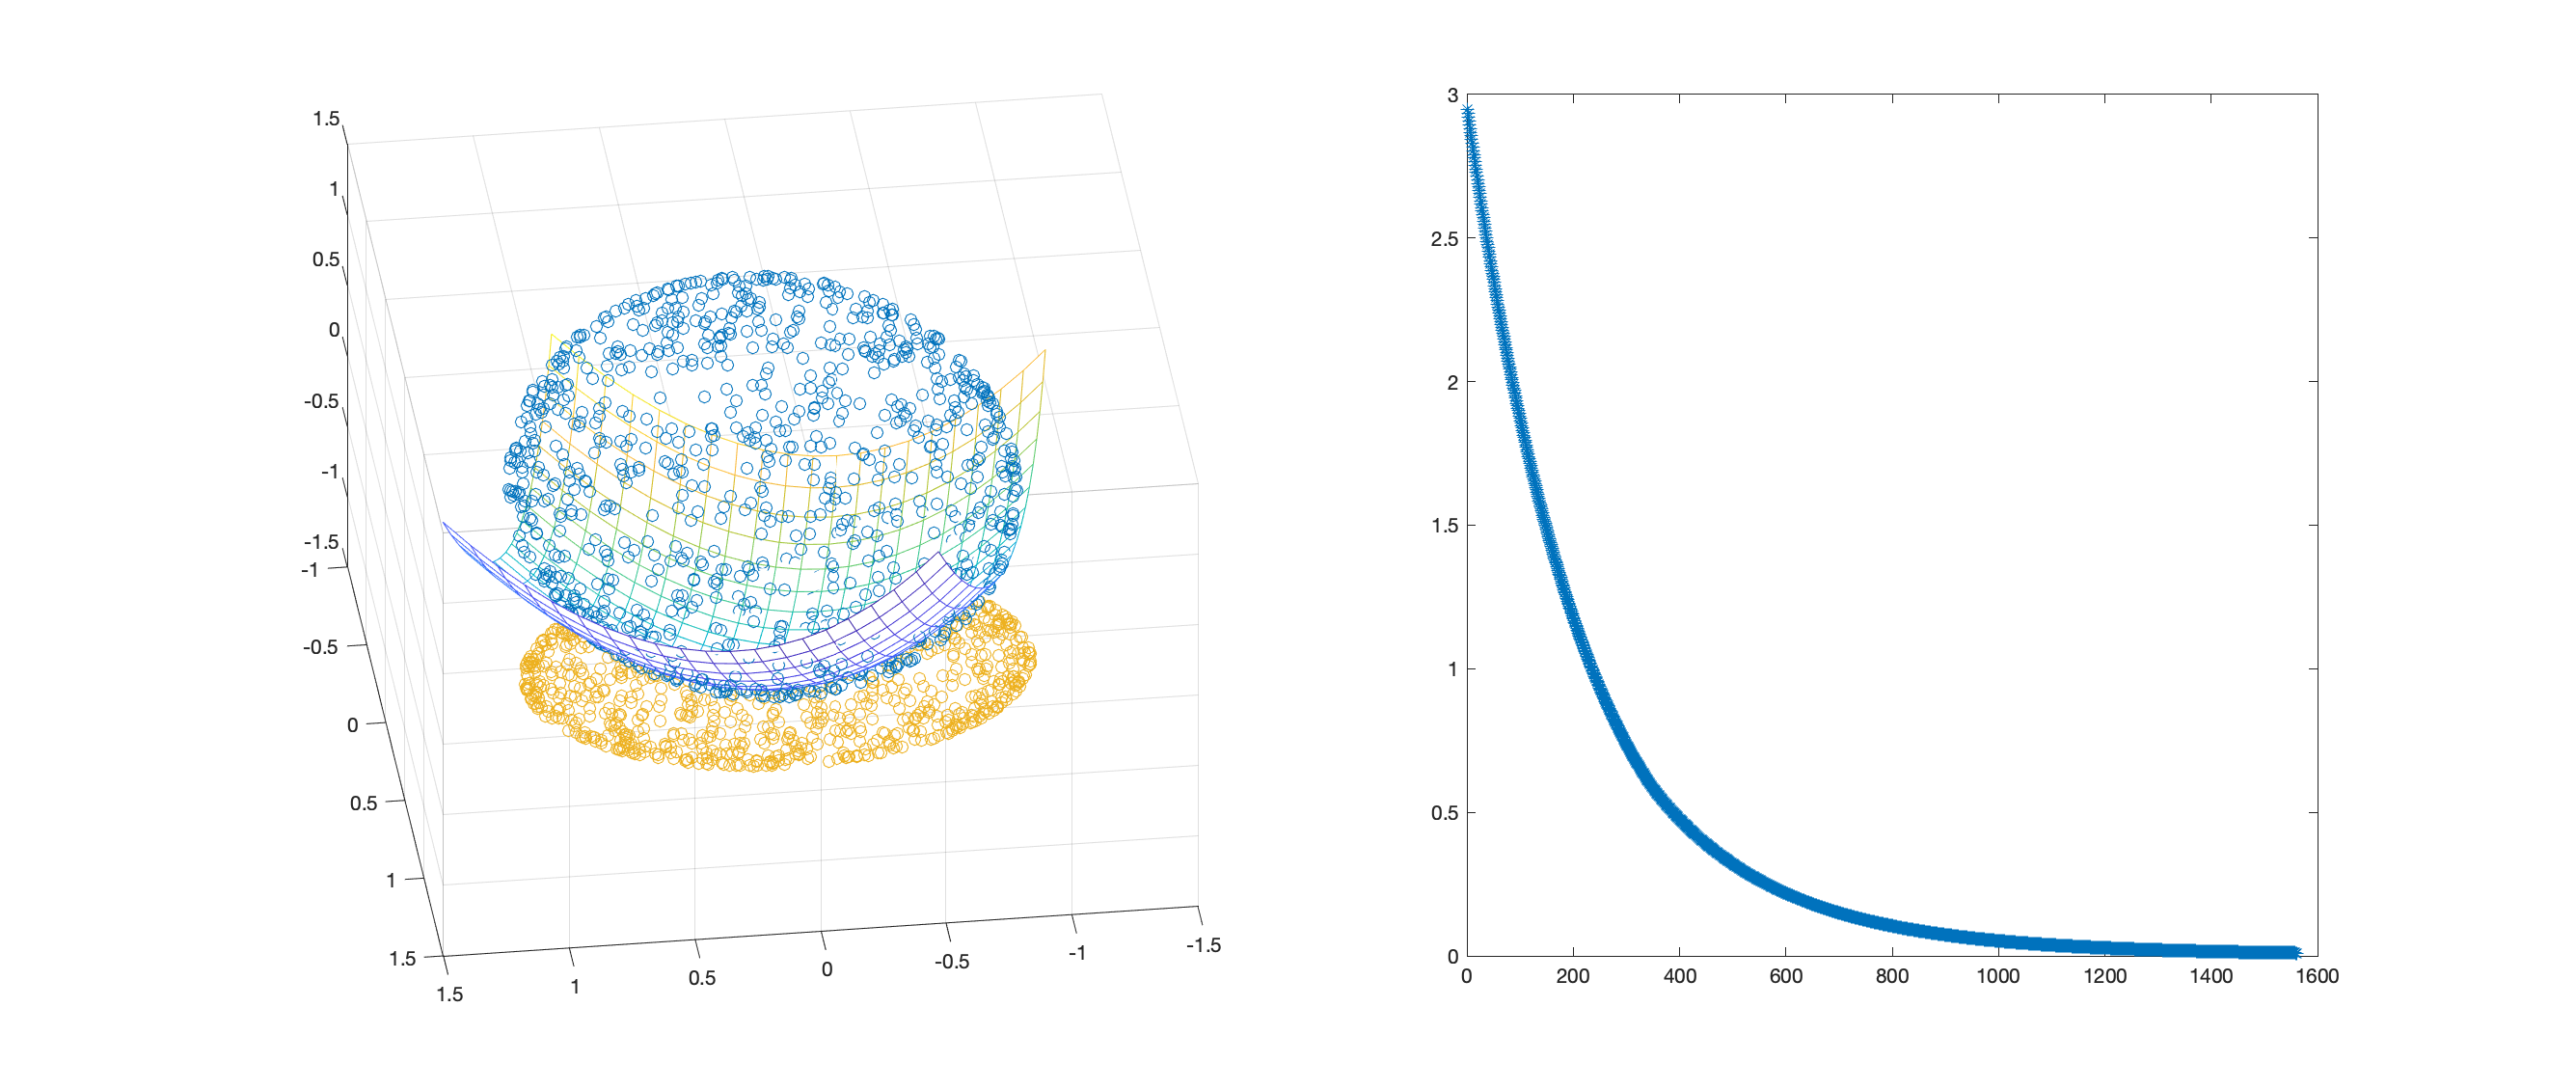
\includegraphics[width=\linewidth]{curvature_fit.eps} 
%   \caption{Left: the fitted second order form. Right: the steepest descend process of the function value of $F(S)$ varies with iteration}
%   \label{fig:example}
%\end{figure}
%\section{Application}

\end{appendix}
%\section{Introduction}
%
%This template helps you to create a properly formatted \LaTeXe\ manuscript.
%%%%%%%%%%%%%%%%%%%%%%%%%%%%%%%%%%%%%%%%%%%%%%
%% `\ ' is used here because TeX ignores    %%
%% spaces after text commands.              %%
%%%%%%%%%%%%%%%%%%%%%%%%%%%%%%%%%%%%%%%%%%%%%%
%Prepare your paper in the same style as used in this sample .pdf file.
%Try to avoid excessive use of italics and bold face.
%Please do not use any \LaTeXe\ or \TeX\ commands that affect the layout
%or formatting of your document (i.e., commands like \verb|\textheight|,
%\verb|\textwidth|, etc.).
%
%\section{Section headings}
%Here are some sub-sections:
%\subsection{A sub-section}
%Regular text.
%\subsubsection{A sub-sub-section}
%Regular text.
%
%\section{Text}
%\subsection{Lists}
%
%The following is an example of an \emph{itemized} list,
%two levels deep.
%\begin{itemize}
%\item
%This is the first item of an itemized list.  Each item
%in the list is marked with a ``tick.''  The document
%style determines what kind of tick mark is used.
%\item
%This is the second item of the list.  It contains another
%list nested inside it.
%\begin{itemize}
%\item This is the first item of an itemized list that
%is nested within the itemized list.
%\item This is the second item of the inner list.  \LaTeX\
%allows you to nest lists deeper than you really should.
%\end{itemize}
%This is the rest of the second item of the outer list.
%\item
%This is the third item of the list.
%\end{itemize}
%
%The following is an example of an \emph{enumerated} list of one level.
%
%\begin{longlist}
%\item This is the first item of an enumerated list.
%\item This is the second item of an enumerated list.
%\end{longlist}
%
%The following is an example of an \emph{enumerated} list, two levels deep.
%\begin{longlist}
%\item[1.]
%This is the first item of an enumerated list.  Each item
%in the list is marked with a ``tick.''  The document
%style determines what kind of tick mark is used.
%\item[2.]
%This is the second item of the list.  It contains another
%list nested inside of it.
%\begin{longlist}
%\item
%This is the first item of an enumerated list that
%is nested within.  
%\item
%This is the second item of the inner list.  \LaTeX\
%allows you to nest lists deeper than you really should.
%\end{longlist}
%This is the rest of the second item of the outer list.
%\item[3.]
%This is the third item of the list.
%\end{longlist}
%
%\subsection{Punctuation}
%Dashes come in three sizes: a hyphen, an intra-word dash like ``$U$-statistics'' or ``the time-homogeneous model'';
%a medium dash (also called an ``en-dash'') for number ranges or between two equal entities like ``1--2'' or ``Cauchy--Schwarz inequality'';
%and a punctuation dash (also called an ``em-dash'') in place of a comma, semicolon,
%colon or parentheses---like this.
%
%Generating an ellipsis \ldots\ with the right spacing
%around the periods requires a special command.
%
%\section{Fonts}
%Please use text fonts in text mode, e.g.:
%\begin{itemize}
%\item[]\textrm{Roman}
%\item[]\textit{Italic}
%\item[]\textbf{Bold}
%\item[]\textsc{Small Caps}
%\item[]\textsf{Sans serif}
%\item[]\texttt{Typewriter}
%\end{itemize}
%Please use mathematical fonts in mathematical mode, e.g.:
%\begin{itemize}
%\item[] $\mathrm{ABCabc123}$
%\item[] $\mathit{ABCabc123}$
%\item[] $\mathbf{ABCabc123}$
%\item[] $\boldsymbol{ABCabc123\alpha\beta\gamma}$
%\item[] $\mathcal{ABC}$
%\item[] $\mathbb{ABC}$
%\item[] $\mathsf{ABCabc123}$
%\item[] $\mathtt{ABCabc123}$
%\item[] $\mathfrak{ABCabc123}$
%\end{itemize}
%Note that \verb|\mathcal, \mathbb| belongs to capital letters-only font typefaces.
%
%\section{Notes}
%Footnotes\footnote{This is an example of a footnote.}
%pose no problem.\footnote{Note that footnote number is after punctuation.}
%
%\section{Quotations}
%
%Text is displayed by indenting it from the left margin. There are short quotations
%\begin{quote}
%This is a short quotation.  It consists of a
%single paragraph of text.  There is no paragraph
%indentation.
%\end{quote}
%and longer ones.
%\begin{quotation}
%This is a longer quotation.  It consists of two paragraphs
%of text.  The beginning of each paragraph is indicated
%by an extra indentation.
%
%This is the second paragraph of the quotation.  It is just
%as dull as the first paragraph.
%\end{quotation}
%
%\section{Environments}
%
%\subsection{Examples for \emph{\texttt{plain}}-style environments}
%\begin{axiom}\label{ax1}
%This is the body of Axiom \ref{ax1}.
%\end{axiom}
%
%\begin{proof}
%This is the body of the proof of the axiom above.
%\end{proof}
%
%\begin{claim}\label{cl1}
%This is the body of Claim \ref{cl1}. Claim \ref{cl1} is numbered after
%Axiom \ref{ax1} because we used \verb|[axiom]| in \verb|\newtheorem|.
%\end{claim}
%
%\begin{theorem}\label{th1}
%This is the body of Theorem \ref{th1}. Theorem \ref{th1} numbering is
%dependent on section because we used \verb|[section]| after \verb|\newtheorem|.
%\end{theorem}
%
%\begin{theorem}[Title of the theorem]\label{th2}
%This is the body of Theorem \ref{th2}. Theorem \ref{th2} has additional title.
%\end{theorem}
%
%\begin{lemma}\label{le1}
%This is the body of Lemma \ref{le1}. Lemma \ref{le1} is numbered after
%Theorem \ref{th2} because we used \verb|[theorem]| in \verb|\newtheorem|.
%\end{lemma}
%
%
%\begin{proof}[Proof of Lemma \ref{le1}]
%This is the body of the proof of Lemma \ref{le1}.
%\end{proof}
%
%\subsection{Examples for \emph{\texttt{remark}}-style environments}
%\begin{definition}\label{de1}
%This is the body of Definition \ref{de1}. Definition \ref{de1} is numbered after
%Lemma \ref{le1} because we used \verb|[theorem]| in \verb|\newtheorem|.
%\end{definition}
%
%\begin{example}
%This is the body of the example. Example is unnumbered because we used \verb|\newtheorem*|
%instead of \verb|\newtheorem|.
%\end{example}
%
%\begin{fact}
%This is the body of the fact. Fact is unnumbered because we used \verb|\newtheorem*|
%instead of \verb|\newtheorem|.
%\end{fact}
%
%\section{Tables and figures}
%Cross-references to labeled tables: As you can see in Table~\ref{sphericcase}
%and also in Table~\ref{parset}.
%
%\begin{table*}
%\caption{The spherical case ($I_1=0$, $I_2=0$)}
%\label{sphericcase}
%\begin{tabular}{@{}lrrrrc@{}}
%\hline
%Equil. \\
%points & \multicolumn{1}{c}{$x$}
%& \multicolumn{1}{c}{$y$} & \multicolumn{1}{c}{$z$}
%& \multicolumn{1}{c}{$C$} & S \\
%\hline
%$L_1$    & $-$2.485252241 & 0.000000000  & 0.017100631  & 8.230711648  & U \\
%$L_2$    & 0.000000000  & 0.000000000  & 3.068883732  & 0.000000000  & S \\
%$L_3$    & 0.009869059  & 0.000000000  & 4.756386544  & $-$0.000057922 & U \\
%$L_4$    & 0.210589855  & 0.000000000  & $-$0.007021459 & 9.440510897  & U \\
%$L_5$    & 0.455926604  & 0.000000000  & $-$0.212446624 & 7.586126667  & U \\
%$L_6$    & 0.667031314  & 0.000000000  & 0.529879957  & 3.497660052  & U \\
%$L_7$    & 2.164386674  & 0.000000000  & $-$0.169308438 & 6.866562449  & U \\
%$L_8$    & 0.560414471  & 0.421735658  & $-$0.093667445 & 9.241525367  & U \\
%$L_9$    & 0.560414471  & $-$0.421735658 & $-$0.093667445 & 9.241525367  & U \\
%$L_{10}$ & 1.472523232  & 1.393484549  & $-$0.083801333 & 6.733436505  & U \\
%$L_{11}$ & 1.472523232  & $-$1.393484549 & $-$0.083801333 & 6.733436505  & U \\
%\hline
%\end{tabular}
%\end{table*}
%
%\begin{table}
%\caption{Sample posterior estimates for each model}
%\label{parset}
%
%\begin{tabular}{@{}lcrcrrr@{}}
%\hline
%&& & &\multicolumn{3}{c}{Quantile} \\
%\cline{5-7}
%Model &Parameter &
%\multicolumn{1}{c}{Mean} &
%Std. dev.&
%\multicolumn{1}{c}{2.5\%} &
%\multicolumn{1}{c}{50\%}&
%\multicolumn{1}{c@{}}{97.5\%} \\
%\hline
%{Model 0} & $\beta_0$ & $-$12.29 & 2.29 & $-$18.04 & $-$11.99 & $-$8.56 \\
%          & $\beta_1$  & 0.10   & 0.07 & $-$0.05  & 0.10   & 0.26  \\
%          & $\beta_2$   & 0.01   & 0.09 & $-$0.22  & 0.02   & 0.16  \\[6pt]
%{Model 1} & $\beta_0$   & $-$4.58  & 3.04 & $-$11.00 & $-$4.44  & 1.06  \\
%          & $\beta_1$   & 0.79   & 0.21 & 0.38   & 0.78   & 1.20  \\
%          & $\beta_2$   & $-$0.28  & 0.10 & $-$0.48  & $-$0.28  & $-$0.07 \\[6pt]
%{Model 2} & $\beta_0$   & $-$11.85 & 2.24 & $-$17.34 & $-$11.60 & $-$7.85 \\
%          & $\beta_1$   & 0.73   & 0.21 & 0.32   & 0.73   & 1.16  \\
%          & $\beta_2$   & $-$0.60  & 0.14 & $-$0.88  & $-$0.60  & $-$0.34 \\
%          & $\beta_3$   & 0.22   & 0.17 & $-$0.10  & 0.22   & 0.55  \\
%\hline
%\end{tabular}
%
%\end{table}
%
%\begin{figure}
%\includegraphics{figure1}
%\caption{Pathway of the penicillin G biosynthesis.}
%\label{penG}
%\end{figure}
%
%Sample of cross-reference to figure.
%Figure~\ref{penG} shows that it is not easy to get something on paper.
%
%\section{Equations and the like}
%
%Two equations:
%\begin{equation}
%    C_{s}  =  K_{M} \frac{\mu/\mu_{x}}{1-\mu/\mu_{x}} \label{ccs}
%\end{equation}
%and
%\begin{equation}
%    G = \frac{P_{\mathrm{opt}} - P_{\mathrm{ref}}}{P_{\mathrm{ref}}}  100(\%).
%\end{equation}
%
%Equation arrays:
%\begin{eqnarray}
%  \frac{dS}{dt} & = & - \sigma X + s_{F} F,\\
%  \frac{dX}{dt} & = &   \mu    X,\\
%  \frac{dP}{dt} & = &   \pi    X - k_{h} P,\\
%  \frac{dV}{dt} & = &   F.
%\end{eqnarray}
%One long equation:
%\begin{eqnarray}
% \mu_{\text{normal}} & = & \mu_{x} \frac{C_{s}}{K_{x}C_{x}+C_{s}}  \nonumber\\
%                     & = & \mu_{\text{normal}} - Y_{x/s}\bigl(1-H(C_{s})\bigr)(m_{s}+\pi /Y_{p/s})\\
%                     & = & \mu_{\text{normal}}/Y_{x/s}+ H(C_{s}) (m_{s}+ \pi /Y_{p/s}).\nonumber
%\end{eqnarray}
%%%%%%%%%%%%%%%%%%%%%%%%%%%%%%%%%%%%%%%%%%%%%%
%% Example with single Appendix:            %%
%%%%%%%%%%%%%%%%%%%%%%%%%%%%%%%%%%%%%%%%%%%%%%
%\begin{appendix}
%\section*{Title}\label{appn} %% if no title is needed, leave empty \section*{}.
%Appendices should be provided in \verb|{appendix}| environment,
%before Acknowledgements.
%
%If there is only one appendix,
%then please refer to it in text as \ldots\ in the \hyperref[appn]{Appendix}.
%\end{appendix}
%%%%%%%%%%%%%%%%%%%%%%%%%%%%%%%%%%%%%%%%%%%%%%
%% Example with multiple Appendixes:        %%
%%%%%%%%%%%%%%%%%%%%%%%%%%%%%%%%%%%%%%%%%%%%%%
%\begin{appendix}
%\section{Title of the first appendix}\label{appA}
%If there are more than one appendix, then please refer to it
%as \ldots\ in Appendix \ref{appA}, Appendix \ref{appB}, etc.
%
%\section{Title of the second appendix}\label{appB}
%\subsection{First subsection of Appendix \protect\ref{appB}}
%
%Use the standard \LaTeX\ commands for headings in \verb|{appendix}|.
%Headings and other objects will be numbered automatically.
%\begin{equation}
%\mathcal{P}=(j_{k,1},j_{k,2},\dots,j_{k,m(k)}). \label{path}
%\end{equation}
%
%Sample of cross-reference to the formula (\ref{path}) in Appendix \ref{appB}.
%\end{appendix}
%
%%%%%%%%%%%%%%%%%%%%%%%%%%%%%%%%%%%%%%%%%%%%%%
%% Support information (funding), if any,   %%
%% should be provided in the                %%
%% Acknowledgements section.                %%
%%%%%%%%%%%%%%%%%%%%%%%%%%%%%%%%%%%%%%%%%%%%%%
%\section*{Acknowledgements}
%The authors would like to thank the anonymous referees, an Associate
%Editor and the Editor for their constructive comments that improved the
%quality of this paper.
%
%The first author was supported by NSF Grant DMS-??-??????.
%
%The second author was supported in part by NIH Grant ???????????.
%
%
%%%%%%%%%%%%%%%%%%%%%%%%%%%%%%%%%%%%%%%%%%%%%%
%% Supplementary Material, if any, should   %%
%% be provided in {supplement} environment  %%
%% with title and short description.        %%
%%%%%%%%%%%%%%%%%%%%%%%%%%%%%%%%%%%%%%%%%%%%%%
%\begin{supplement}
%\textbf{Title of Supplement A}.
%Short description of Supplement A.
%\end{supplement}
%\begin{supplement}
%\textbf{Title of Supplement B}.
%Short description of Supplement B.
%\end{supplement}
%
%%%%%%%%%%%%%%%%%%%%%%%%%%%%%%%%%%%%%%%%%%%%%%%%%%%%%%%%%%%%%
%%                  The Bibliography                       %%
%%                                                         %%
%%  imsart-???.bst  will be used to                        %%
%%  create a .BBL file for submission.                     %%
%%                                                         %%
%%  Note that the displayed Bibliography will not          %%
%%  necessarily be rendered by Latex exactly as specified  %%
%%  in the online Instructions for Authors.                %%
%%                                                         %%
%%  MR numbers will be added by VTeX.                      %%
%%                                                         %%
%%  Use \cite{...} to cite references in text.             %%
%%                                                         %%
%%%%%%%%%%%%%%%%%%%%%%%%%%%%%%%%%%%%%%%%%%%%%%%%%%%%%%%%%%%%%
%
%% if your bibliography is in bibtex format, uncomment commands:
\bibliographystyle{imsart-nameyear} % Style BST file (imsart-number.bst or imsart-nameyear.bst)
\bibliography{bibfile}       % Bibliography file (usually '*.bib')
%
%% or include bibliography directly:
%\begin{thebibliography}{4}
%%
%\bibitem{r1}
%\textsc{Billingsley, P.} (1999). \textit{Convergence of
%Probability Measures}, 2nd ed.
%Wiley, New York.
%
%\bibitem{r2}
%\textsc{Bourbaki, N.}  (1966). \textit{General Topology}  \textbf{1}.
%Addison--Wesley, Reading, MA.
%
%\bibitem{r3}
%\textsc{Ethier, S. N.} and \textsc{Kurtz, T. G.} (1985).
%\textit{Markov Processes: Characterization and Convergence}.
%Wiley, New York.
%
%\bibitem{r4}
%\textsc{Prokhorov, Yu.} (1956).
%Convergence of random processes and limit theorems in probability
%theory. \textit{Theory  Probab.  Appl.}
%\textbf{1} 157--214.
%\end{thebibliography}

\end{document}
